\documentclass[12pt,oneside]{book}
\usepackage{import}
%===============================%
%  Packages and basic settings  %
%===============================%
\usepackage[headheight=15pt,rmargin=0.5in,lmargin=0.5in,tmargin=0.75in,bmargin=0.75in]{geometry}
\usepackage{imakeidx}
\usepackage{framed}
\usepackage{amssymb}
\usepackage{amsmath}
\usepackage{mathrsfs}
\usepackage{enumitem}
\usepackage{hyperref}
\usepackage{appendix}
\usepackage[capitalise,noabbrev]{cleveref}
\usepackage{tikz}
\usepackage{tikz-cd}
\usepackage{nomencl}\makenomenclature
\usetikzlibrary{braids,arrows,decorations.markings,calc}

%====================================%
%  Theorems, environments & cleveref  %
%====================================%
\newtheorem{theorem}{Theorem}[section]
\newtheorem{proposition}{Proposition}[section]
\newtheorem{corollary}{Corollary}[section]
\newtheorem{lemma}{Lemma}[section]
\newtheorem{conjecture}{Conjecture}[section]
\newtheorem{remark}{Remark}[section]

\newenvironment{stabular}[2][1]
  {\def\arraystretch{#1}\tabular{#2}}
  {\endtabular}

%==================================%
%  Custom commands & environments  %
%==================================%
\newcommand{\legendre}[2]{\left(\frac{#1}{#2}\right)}
\newcommand{\dlegendre}[2]{\displaystyle{\left(\frac{#1}{#2}\right)}}
\newcommand{\tlegendre}[2]{\textstyle{\left(\frac{#1}{#2}\right)}}
\newcommand{\psum}{\sideset{}{'}\sum}
\newcommand{\asum}{\sideset{}{^{\ast}}\sum}
\newcommand{\tmod}[1]{\ \left(\text{mod }#1\right)}
\newcommand{\xto}[1]{\xrightarrow{#1}}
\newcommand{\xfrom}[1]{\xleftarrow{#1}}
\newcommand{\normal}{\mathrel{\unlhd}}
\newcommand{\mf}{\mathfrak}
\newcommand{\mc}{\mathcal}
\newcommand{\ms}{\mathscr}

\newcommand{\Mat}{\mathrm{Mat}}
\newcommand{\GL}{\mathrm{GL}}
\newcommand{\SL}{\mathrm{SL}}
\newcommand{\PSL}{\mathrm{PSL}}
\renewcommand{\O}{\mathrm{O}}
\newcommand{\SO}{\mathrm{SO}}
\newcommand{\U}{\mathrm{U}}
\newcommand{\Sp}{\mathrm{Sp}}

\newcommand{\N}{\mathbb{N}}
\newcommand{\Z}{\mathbb{Z}}
\newcommand{\Q}{\mathbb{Q}}
\newcommand{\R}{\mathbb{R}}
\newcommand{\C}{\mathbb{C}}
\newcommand{\F}{\mathbb{F}}
\renewcommand{\H}{\mathbb{H}}
\renewcommand{\P}{\mathbb{P}}

\renewcommand{\a}{\alpha}
\renewcommand{\b}{\beta}
\newcommand{\g}{\gamma}
\renewcommand{\d}{\delta}
\newcommand{\z}{\zeta}
\renewcommand{\t}{\theta}
\renewcommand{\i}{\iota}
\renewcommand{\k}{\kappa}
\renewcommand{\l}{\lambda}
\newcommand{\s}{\sigma}
\newcommand{\w}{\omega}

\newcommand{\G}{\Gamma}
\newcommand{\D}{\Delta}
\renewcommand{\L}{\Lambda}
\newcommand{\W}{\Omega}

\newcommand{\e}{\varepsilon}
\newcommand{\vt}{\vartheta}
\newcommand{\vphi}{\varphi}
\newcommand{\emt}{\varnothing}

\newcommand{\x}{\times}
\newcommand{\ox}{\otimes}
\newcommand{\op}{\oplus}
\newcommand{\bigox}{\bigotimes}
\newcommand{\bigop}{\bigoplus}
\newcommand{\del}{\partial}
\newcommand{\<}{\langle}
\renewcommand{\>}{\rangle}
\newcommand{\lf}{\lfloor}
\newcommand{\rf}{\rfloor}
\newcommand{\wtilde}{\widetilde}
\newcommand{\what}{\widehat}
\newcommand{\conj}{\overline}
\newcommand{\cchi}{\conj{\chi}}

\DeclareMathOperator{\id}{\textrm{id}}
\DeclareMathOperator{\sgn}{\mathrm{sgn}}
\DeclareMathOperator{\im}{\mathrm{im}}
\DeclareMathOperator{\rk}{\mathrm{rk}}
\DeclareMathOperator{\tr}{\mathrm{trace}}
\DeclareMathOperator{\nm}{\mathrm{norm}}
\DeclareMathOperator{\ord}{\mathrm{ord}}
\DeclareMathOperator{\Hom}{\mathrm{Hom}}
\DeclareMathOperator{\End}{\mathrm{End}}
\DeclareMathOperator{\Aut}{\mathrm{Aut}}
\DeclareMathOperator{\Tor}{\mathrm{Tor}}
\DeclareMathOperator{\Ann}{\mathrm{Ann}}
\DeclareMathOperator{\Gal}{\mathrm{Gal}}
\DeclareMathOperator{\Trace}{\mathrm{Trace}}
\DeclareMathOperator{\Norm}{\mathrm{Norm}}
\DeclareMathOperator{\Span}{\mathrm{Span}}
\DeclareMathOperator*{\Res}{\mathrm{Res}}
\DeclareMathOperator{\Vol}{\mathrm{Vol}}
\DeclareMathOperator{\Li}{\mathrm{Li}}
\renewcommand{\Re}{\mathrm{Re}}
\renewcommand{\Im}{\mathrm{Im}}

\newcommand{\GH}{\G\backslash\H}
\newcommand{\GG}{\G_{\infty}\backslash\G}

\newenvironment{psmallmatrix}
  {\left(\begin{smallmatrix}}
  {\end{smallmatrix}\right)}

%============%
%  Comments  %
%============%
\newcommand{\todo}[1]{\textcolor{red}{\sf Todo: [#1]}}

%===================%
%  Label reminders  %
%===================%
% [label=(\roman*)]
% [label=(\alph*)]
% [label=(\arabic{enumi})]

%==================%
%  Other settings  %
%==================%
\pgfdeclarelayer{background}
\pgfsetlayers{background,main}
\tikzset{->-/.style={decoration={
  markings,
  mark=at position .5 with {\arrow{>}}},postaction={decorate}}}

%=================%
%  Title & Index  %
%=================%
\title{An Introduction to Multiple Dirichlet Series}
\author{Jeff Hoffstein, Henry Twiss, \todo{XXX}}
\date{2024}
\makeindex

\begin{document}
\maketitle
\pagestyle{empty}
\addtocontents{toc}{\protect\thispagestyle{empty}}
\tableofcontents
\setcounter{page}{0}
\pagestyle{fancy}

\chapter{Historical Context}

\chapter{The Heuristic Argument}

\chapter{Quadratic Double Dirichlet Series I: The Function Field Case}
  \section{Preliminaries}
    We will give an overview of the zeta function and quadratic Dirichlet $L$-functions attached to $\F_{q}(t)$. For proofs of these facts and a more detailed analysis see \cite{rosen2002number}. Let $q$ be a power of an odd prime and let $\F_{q}[t]$ be the polynomial ring in $t$ with coefficients in the finite field $\F_{q}$. This is a principal ideal domain. Moreover, the nonzero prime ideals in $\F_{q}[t]$ are generated by irreducible polynomials. Let $\F_{q}(t)$ denote the quotient field. Define the norm function $N(m)$ by
    \[
        N(m) = |m| = q^{\deg(m)},
    \]
    for any $m \in \F_{q}[t]$. The zeta function $\z(s)$ on $\F_{q}[t]$ is defined as the Dirichlet series or Euler product
    \[
        \z(s) = \sum_{\text{$m$ monic}}\frac{1}{|m|^{s}} = \prod_{\text{$P$ monic irr}}\left(1-\frac{1}{|P|^{s}}\right)^{-1},
    \]
    where the second equality holds since $\F_{q}[t]$ is a unique factorization domain. As for questions of convergence, there are $q^{n}$ monic polynomials of degree $n$ so, provided $\Re(s) > 1$, we can sum up the Dirichlet series according to degree and obtain an explicit expression:
    \[
        \z(s) = \sum_{n \ge 0}\frac{\text{\# of monic poly of deg $n$}}{q^{ns}} = \sum_{n \ge 1}\frac{1}{q^{n(1-s)}} = \frac{1}{1-q^{1-s}}.
    \]
    The latter expression is meromorphic on $\C$ with a simple pole at $s = 1$ of residue $\frac{1}{\log(q)}$. Therefore $\z(s)$ admits meromorphic continuation to $\C$. The zeta function also satisfies a functional equation. Define the completed zeta function $\z^{\ast}(s)$ (this is also the zeta function attached to $\F_{q}(t)$) by
    \[
        \z^{\ast}(s) = \frac{1}{1-q^{-s}}\z(s).
    \]
    Then
    \[
        \z^{\ast}(s) = q^{2s-1}\z^{\ast}(1-s).
    \]
    Recall that characters on $\F_{q}[t]$ are multiplicative functions $\chi:\F_{q}[t] \to \C$. They form a group under multiplication. The two flavors we will care about are:
    
    \begin{itemize}
        \item Dirichlet characters: multiplicative functions $\chi_{d}:\F_{q}[t] \to \C$ modulo $d \in \F_{q}[t]$ (in that they are $d$-periodic) and such that $\chi_{d}(m) = 0$ if $(m,d) > 1$.
        \item Hilbert characters: The group of characters generated by those that appear in the sign change of reciprocity statements.
    \end{itemize}
    
    The image of a Dirichlet character always lands in the roots of unity. Moreover, $\conj{\chi}$ is the multiplicative inverse to $\chi$ and the Dirichlet characters modulo $d$ form a subgroup under multiplication. This group is always finite and its order is $\phi(d) = |(\F_{q}[t]/d\F_{q}[t])^{\x}|$. The Dirichlet characters that are of interest to us are those attached to quadratic extensions of $\F_{q}[t]$ which, in turn, arise from the quadratic residue symbol. First let us recall this symbol. For any irreducible $p \in \F_{q}[t]$ and any $d \in \F_{q}[t]$, we define the quadratic residue symbol $\tlegendre{d}{p}$ by
    \[
        \legendre{d}{p} \equiv d^{\frac{|p|-1}{2}} \tmod{p} = \begin{cases} 1 & \text{if $x^{2} \equiv d \tmod{p}$ is solvable}, \\ -1 & \text{if $x^{2} \equiv d \tmod{p}$ is not solvable}, \\ 0 & \text{if $d \equiv 0 \tmod{p}$}. \end{cases}
    \]
    This symbol is only dependent upon $d$ modulo $p$ and is multiplicative in $d$. Moreover, if $b \in \F_{q}^{\ast}$, we have
    \[
        \legendre{b}{p} = \sgn(b)^{\deg(p)}.
    \]
    where $\sgn(b) = \pm1$ depending on if $b \in (\F_{q}^{\x})^{2}$ or not. Moreover, for $d \in \F_{q}[t]$ we have $\sgn(d) = \sgn(b_{n})$ if $d(t) = b_{n}t^{n}+b_{n-1}t^{n+1}+\cdots+b_{0}$ (with $b_{n} \neq 0$). We can extend the quadratic residue symbol multiplicatively in the denominator. If $m = bp_{1}^{e_{1}}p_{2}^{e_{2}} \cdots p_{k}^{e_{k}}$ is the prime factorization of $m$ (with $b \in \F_{q}^{\ast}$), then we define
    \[
        \legendre{d}{m} = \prod_{1 \le i \le k}\legendre{d}{p_{i}}^{e_{i}}.
    \]
    So the quadratic residue symbol now makes sense for any nonzero $m \in \F_{q}[t]$. Morevoer, it only depends upon $d$ modulo $m$, the ideal generated by $m$, and is multiplicative in $m$. The quadratic residue symbol also admits the following reciprocity law:

    \begin{theorem}[Quadratic reciprocity]
        If $d,m \in \F_{q}[t]$ are nonzero, then
        \[
            \legendre{d}{m} = (-1)^{\frac{q-1}{2}\deg(d)\deg(m)}\sgn(d)^{\deg(m)}\sgn(m)^{-\deg(d)}\legendre{m}{d}.
        \]
    \end{theorem}

    Note that if $q \equiv 1 \tmod{4}$ and $d$ and $m$ are monic, then the sign in the statement of quadratic reciprocity is always $1$ so that reciprocity is perfect:
    \[
        \legendre{d}{m} = \legendre{m}{d}.
    \]
    We can now define the quadratic Dirichlet characters. For any nonzero square-free monic $d \in \F_{q}[t]$, define the quadratic Dirichlet character $\chi_{d}$ by the following quadratic residue symbol:
    \[
        \chi_{d}(m) = \legendre{d}{m}.
    \]
    This quadratic Dirichlet character is attached to the quadratic extension $\F_{q}(t)(\sqrt{d})$. If $b \in \F_{q}^{\x}$, we define $\chi_{b}$ by
    \[
        \chi_{b}(m) = \legendre{b}{m} = \sgn(b)^{\deg(m)}.
    \]
    We extend $\chi_{d}$ multiplicatively in the denominator so that $\chi_{d}$ makes sense for any nonzero $d \in \F_{q}[t]$. In particular, $\chi_{d}(m) = \pm1$ provided $d$ and $m$ are relatively prime and $\chi_{d}(m) = 0$ if $(m,d) > 1$. Quadratic reciprocity implies that $\chi_{d}$ is a Dirichlet character modulo $d$. Indeed, for any $m$ we can take $d$ modulo $m$ so that $\deg(d+m) = \deg(m)$ and $\sgn(d+m) = \sgn(m)$. Lastly, note that if $q \equiv 1 \tmod{4}$ and $d$ and $m$ are monic, then
    \[
        \chi_{d}(m) = \chi_{m}(d),
    \]
    which is a reformulation of reciprocity being perfect. We now discuss the Hilbert characters. We will only need two of them: one nontrivial and one trivial. The nontrivial Hilbert character is $\chi_{\t}$ where $\t \in \F^{\x}-(\F^{\x})^{2}$:
    \[
        \chi_{\t}(m) = (-1)^{\deg(m)}.
    \]
    Note that $\conj{\chi_{\t}} = \chi_{\t}$. The other Hilbert character is the trivial Dirichlet character $\chi_{\t}^{2} = \chi_{\t\t} = \chi_{1}$. In general, we denote a Hilbert character by $\chi_{a}$ where $a \in \{1,\t\}$. The Hilbert characters also satisfy an important orthogonality property:

    \begin{theorem}[Orthogonality of Hilbert characters]
        If $d,m \in \F_{q}[t]$ are nonzero, then
        \[
            \frac{1}{2}\sum_{a \in \{1,\t\}}\chi_{a}(dm) = \begin{cases} 1 & \text{if $\deg(d) \equiv \deg(m) \tmod{2}$}, \\ 0 & \text{if $\deg(d) \not\equiv \deg(m) \tmod{2}$}. \end{cases}
        \]
    \end{theorem}
    
    More generally, we would also require Hilbert characters to keep track of the $(-1)^{\frac{q-1}{2}\deg(d)\deg(m)}$ factor in the statement of quadratic reciprocity but as we will assume $q \equiv 1 \tmod{4}$, we will not require this additional difficulty. With the Dirichlet and Hilbert characters introduced, we are ready to discuss the $L$-functions associated to quadratic Dirichlet characters. We define the Dirichlet $L$-function $L(s,\chi_{d})$ attached to $\chi_{d}$ for square-free $d$, by a Dirichlet series or Euler product:
    \[
        L(s,\chi_{d}) = \sum_{\text{$m$ monic}}\frac{\chi_{d}(m)}{|m|^{s}} = \prod_{\text{$P$ monic irr}}\left(1-\frac{\chi_{d}(P)}{|P|^{s}}\right)^{-1}.
    \]
    By definition of the quadratic Dirichlet character, $L(s,\chi_{d}) \ll \z(s)$ for $\Re(s) > 1$ so that $L(s,\chi_{d})$ is locally absolutely uniformly convergent in this region. $L(s,\chi_{d})$ also admits analytic continuation to $\C$ (see \cite{rosen2002number} for a proof). Moreover, $L(s,\chi_{d})$ is a polynomial in $q^{-s}$ of degree at most $\deg(d)-1$. The associated completed Dirichlet $L$-function $L^{\ast}(s,\chi_{d})$ is defined as
    \[
        L^{\ast}(s,\chi_{d}) = \begin{cases} \frac{1}{1-q^{-s}}L(s,\chi_{d}) & \text{if $\deg(d)$ is even}, \\ L(s,\chi_{d}) & \text{if $\deg(d)$ is odd}, \end{cases}
    \]
    and satisfies the functional equation
    \[
        L^{\ast}(s,\chi_{d}) = \begin{cases} q^{2s-1}|d|^{\frac{1}{2}-s}L^{\ast}(1-s,\chi_{d}) & \text{if $\deg(d)$ is even}, \\ q^{2s-1}(q|d|)^{\frac{1}{2}-s}L^{\ast}(1-s,\chi_{d}) & \text{if $\deg(d)$ is odd}. \end{cases}
    \]
    Note that in the case $\deg(d)$ is even, the conductor is $|d|$ and in the case $\deg(d)$ is odd, the conductor is $q|d|$. Moreover, the gamma factors depend upon the degree of $d$. This will cause a small but important technical issue later when we want to derive functional equations for the quadratic double Dirichlet series. Analogously (this is a superfluous definition but we are giving it to be consistent with notation for the quadratic double Dirichlet series later on), we define the Dirichlet $L$-function $L(w,\chi_{m})$ attached to $\chi_{m}$ for square-free $m$, by a Dirichlet series or Euler product:
    \[
        L(w,\chi_{m}) = \sum_{\text{$d$ monic}}\frac{\chi_{m}(d)}{|d|^{w}} = \prod_{\text{$P$ monic irr}}\left(1-\frac{\chi_{m}(P)}{|P|^{w}}\right)^{-1}.
    \]
    As for $L(s,\chi_{d})$, $L(w,\chi_{m}) \ll \z(w)$ for $\Re(w) > 1$ so that $L(w,\chi_{m})$ is locally absolutely uniformly convergent in this region. Morevoer, $L(w,\chi_{m})$ admits analytic continuation to $\C$ and is a polynomial in $q^{-w}$ of degree at most $\deg(m)-1$. The associated completed Dirichlet $L$-function $L^{\ast}(w,\chi_{m})$ is defined as
    \[
        L^{\ast}(w,\chi_{m}) = \begin{cases} \frac{1}{1-q^{-w}}L(w,\chi_{m}) & \text{if $\deg(m)$ is even}, \\ L(w,\chi_{m}) & \text{if $\deg(m)$ is odd}, \end{cases}
    \]
    and satisfies the functional equation
    \[
        L^{\ast}(w,\chi_{m}) = \begin{cases} q^{2w-1}|d|^{\frac{1}{2}-w}L^{\ast}(1-w,\chi_{m}) & \text{if $\deg(m)$ is even}, \\ q^{2w-1}(q|m|)^{\frac{1}{2}-w}L^{\ast}(1-w,\chi_{m}) & \text{if $\deg(m)$ is odd}. \end{cases}
    \]

    \begin{remark}
        The definitions for $L(s,\chi_{d})$, $L^{\ast}(s,\chi_{d})$, $L(w,\chi_{m})$, and $L^{\ast}(w,\chi_{m})$ hold even when $d$ and $m$ are not square-free (however the functional equations do not hold). We will make use of slightly modified definitions in this case and so we purposely do not define these $L$-functions yet.
    \end{remark}
\section{The Quadratic Double Dirichlet Series}
    From now on we assume $q \equiv 1 \tmod{4}$. This assumption is not strictly necessary to build the quadratic double Dirichlet series but it does allow for some technical simplifications as the statement of quadratic reciprocity is perfect. We are ready to define the quadratic double Dirichlet series $Z(s,w)$. For any monic $d \in \F_{q}[t]$, write $d = d_{0}d_{1}^{2}$ where $d_{0}$ is square-free. In other words, $d_{0}$ is the square-free part of $d$ so that $\frac{d}{d_{0}}$ is a perfect square. The \textbf{quadratic double Dirichlet series} $Z(s,w)$ is defined as
    \[
        Z(s,w) = \sum_{\text{$d$ monic}}\frac{L(s,\chi_{d_{0}})Q_{d_{0}d_{1}^{2}}(s)}{|d|^{w}},
    \]
    where $Q_{d_{0}d_{1}^{2}}(s)$ is the \textbf{correction polynomial} defined by
    \[
        Q_{d_{0}d_{1}^{2}}(s) = \sum_{e_{1}e_{2} \mid d_{1}}\mu(e_{1})\chi_{d_{0}}(e_{1})|e_{1}|^{-s}|e_{2}|^{1-2s} = \sum_{e_{1}e_{2}e_{3} = d_{1}}\mu(e_{1})\chi_{d_{0}}(e_{1})|e_{1}|^{-s}|e_{2}|^{1-2s},
    \]
    and $\mu$ is the usual M\"obius function on $\F_{q}[t]$. For $\Re(s) > 1$, we have the trivial bound
    \[
        Q_{d_{0}d_{1}^{2}}(s) \ll \sum_{e_{1}e_{2} \mid d_{1}}1 \ll \s_{0}(d_{1})^{2} \ll_{\e} |d_{1}|^{2\e} \ll_{\e} |d|^{\e},
    \]
    for any $\e > 0$. Combining this estimate with the bound $L(s,\chi_{d_{0}}) \ll 1$ for $\Re(s) > 1$, we see that $Z(s,w)$ is locally absolutely uniformly convergent in the region $\L = \{(s,w) \in \C^{2}:\Re(s) > 1, \Re(w) > 1\}$. While $Z(s,w)$ is the double Dirchlet series we are after, it will be necessary to consider quadratic double Dirichlet series twisted by a pair of Hilbert characters $\chi_{a_{1}}$ and $\chi_{a_{2}}$. The \textbf{quadratic double Dirichlet series} $Z_{a_{1},a_{2}}(s,w)$ twisted by $\chi_{a_{1}}$ and $\chi_{a_{2}}$ is defined as
    \[
        Z_{a_{1},a_{2}}(s,w) = \sum_{\text{$d$ monic}}\frac{L(s,\chi_{a_{1}d_{0}})\chi_{a_{2}}(d)Q_{d_{0}d_{1}^{2}}(s,\chi_{a_{1}})}{|d|^{w}},
    \]
    where $Q_{d_{0}d_{1}^{2}}(s,\chi_{a_{1}})$ is the \textbf{correction polynomial} twisted by $\chi_{a_{1}}$ defined by
    \[
        Q_{d_{0}d_{1}^{2}}(s,\chi_{a_{1}}) = \sum_{e_{1}e_{2} \mid d_{1}}\mu(e_{1})\chi_{a_{1}d_{0}}(e_{1})|e_{1}|^{-s}|e_{2}|^{1-2s} = \sum_{e_{1}e_{2}e_{3} = d_{1}}\mu(e_{1})\chi_{a_{1}d_{0}}(e_{1})|e_{1}|^{-s}|e_{2}|^{1-2s},
    \]
    and $\mu$ is the usual M\"obius function on $\F_{q}[t]$. As the Hilbert characters are given by quadratic Dirichlet characters, we have the analogous bound $Q_{d_{0}d_{1}^{2}}(s,\chi_{a_{1}}) \ll |d|_{\e}$ so that $Z_{a_{1},a_{2}}(s,w)$ converges locally absolutely uniformly in the same region as $Z(s,w)$ does. In this generalized setup, $Z(s,w) = Z_{1,1}(s,w)$. Analogously, writing $m = m_{0}m_{1}^{2}$, the \textbf{quadratic double Dirichlet series} $Z(w,s)$ is defined as
    \[
        Z(w,s) = \sum_{\text{$m$ monic}}\frac{L(w,\chi_{m_{0}})Q_{m_{0}m_{1}^{2}}(w)}{|m|^{s}},
    \]
    where $Q_{m_{0}m_{1}^{2}}(w)$ is the \textbf{correction polynomial} defined by
    \[
        Q_{m_{0}m_{1}^{2}}(w) = \sum_{e_{1}e_{2} \mid m_{1}}\mu(e_{1})\chi_{m_{0}}(e_{1})|e_{1}|^{-w}|e_{2}|^{1-w} = \sum_{e_{1}e_{2}e_{3} = m_{1}}\mu(e_{1})\chi_{m_{0}}(e_{1})|e_{1}|^{-w}|e_{2}|^{1-w},
    \]
    and $\mu$ is the usual M\"obius function. We have the analogous estimate $Q_{m_{0}m_{1}^{2}}(w) \ll_{\e} |m|^{\e}$ and since $L(w,\chi_{m_{0}}) \ll 1$ for $\Re(w) > 1$, $Z(w,s)$ is absolutely convergent in the same region as $Z(s,w)$. We will also consider twists by Hilbert characters $\chi_{a_{2}}$ and $\chi_{a_{1}}$. The \textbf{quadratic double Dirichlet series} $Z_{a_{2},a_{1}}(w,s)$ twisted by $\chi_{a_{2}}$ and $\chi_{a_{1}}$ is defined as
    \[
        Z_{a_{2},a_{1}}(w,s) = \sum_{\text{$m$ monic}}\frac{L(w,\chi_{a_{2}m_{0}})\chi_{a_{1}}(m)Q_{m_{0}m_{1}^{2}}(w,\chi_{a_{2}})}{|m|^{s}},
    \]
    where $Q_{m_{0}m_{1}^{2}}(w,\chi_{a_{2}})$ is the \textbf{correction polynomial} twisted by $\chi_{a_{2}}$ defined by
    \[
        Q_{m_{0}m_{1}^{2}}(w,\chi_{a_{2}}) = \sum_{e_{1}e_{2} \mid m_{1}}\mu(e_{1})\chi_{a_{2}m_{0}}(e_{1})|e_{1}|^{-w}|e_{2}|^{1-2w} = \sum_{e_{1}e_{2}e_{3} = m_{1}}\mu(e_{1})\chi_{a_{2}m_{0}}(e_{1})|e_{1}|^{-w}|e_{2}|^{1-2w},
    \]
    and $\mu$ is the usual M\"obius function. Again, we have the analogous bound $Q_{m_{0}m_{1}^{2}}(w,\chi_{a_{2}}) \ll_{\e} |m|^{\e}$ so that $Z_{a_{2},a_{1}}(w,s)$ converges locally absolutely uniformly in the same region as $Z(w,s)$. In particular, $Z(w,s) = Z_{1,1}(w,s)$.
\section{The Interchange}
    Since $L$-functions attached to quadratic Dirichlet characters admit Euler products, $Z_{a_{1},a_{2}}(s,w)$ is a sum of Euler products in $s$. We will now argue that $Z_{a_{1},a_{2}}(s,w)$ can be written as a sum of Euler products in $w$. In effect, we want the variable $s$ to appear in the denominator of $Z_{a_{1},a_{2}}(s,w)$ and the $L$-functions in the numerator to be in the variable $w$. To be precise, we will prove the following:

    \begin{theorem}[Interchange]
        Wherever $Z_{a_{1},a_{2}}(s,w)$ converges locally absolutely uniformly,
        \[
            Z_{a_{1},a_{2}}(s,w) = \sum_{\text{$d$ monic}}\frac{L(s,\chi_{a_{1}d_{0}})\chi_{a_{2}}(d)Q_{d_{0}d_{1}^{2}}(s,\chi_{a_{1}})}{|d|^{w}} = \sum_{\text{$m$ monic}}\frac{L(w,\chi_{a_{2}m_{0}})\chi_{a_{1}}(m)Q_{m_{0}m_{1}^{2}}(w,\chi_{a_{2}})}{|m|^{s}}.
        \]
        Moreover, the same holds for $Z_{a_{2},a_{1}}(w,s)$.
    \end{theorem}
    \begin{proof}
        Only the second equality needs to be justified since the first is the definition of $Z(s,w)$. Expanding the $L$-function $L(s,\chi_{a_{1}d_{0}})$ and polynomial $Q_{d_{0}d_{1}^{2}}(s,\chi_{a_{1}})$ gives
        \begin{align*}
            Z(s,w) &= \sum_{\text{$d$ monic}}\frac{L(s,\chi_{a_{1}d_{0}})\chi_{a_{2}}(d)Q_{d_{0}d_{1}^{2}}(s,\chi_{a_{1}})}{|d|^{w}} \\
            &= \sum_{\text{$d$ monic}}\left(\sum_{\text{$m$ monic}}\chi_{a_{1}d_{0}}(m)|m|^{-s}\right)\left(\sum_{e_{1}e_{2} \mid d_{1}}\mu(e_{1})\chi_{a_{1}d_{0}}(e_{1})|e_{1}|^{-s}|e_{2}|^{1-2s}\right)\chi_{a_{2}}(d)|d|^{-w} \\
            &= \sum_{\text{$m,d$ monic}}\sum_{e_{1}e_{2} \mid d_{1}}\mu(e_{1})\chi_{a_{2}}(d)\chi_{a_{1}d_{0}}(me_{1})|e_{1}|^{-s}|e_{2}|^{1-2s}|m|^{-s}|d|^{-w}.
        \end{align*}
        Now $\chi_{a_{1}d_{0}}(me_{1}) = 0$ unless $(d_{0},me_{1}) = 1$. So we may make this restriction on the sum giving
        \[
            \sum_{\text{$m,d$ monic}}\sum_{\substack{e_{1}e_{2} \mid d_{1} \\ (d_{0},me_{1}) = 1}}\mu(e_{1})\chi_{a_{2}}(d)\chi_{a_{1}d_{0}}(me_{1})|e_{1}|^{-s}|e_{2}|^{1-2s}|m|^{-s}|d|^{-w}.
        \]
        Making the change of variables $me_{1} \to m$ yields
        \[
            \sum_{\text{$d$ monic}}\sum_{\substack{\text{$m$ monic} \\ e_{1} \mid m}}\sum_{\substack{e_{1}e_{2} \mid d_{1} \\ (d_{0},m) = 1}}\mu(e_{1})\chi_{a_{2}}(d)\chi_{a_{1}d_{0}}(m)|e_{2}|^{1-2s}|m|^{-s}|d|^{-w}.
        \]
        Now for fixed $d = d_{0}d_{1}^{2}$ and $e_{2}$, the resulting subsum over $m$ and $e_{1}$ is
        \[
            \sum_{\substack{\text{$m$ monic} \\ e_{1} \mid m}}\sum_{\substack{e_{1} \mid \frac{d_{1}}{e_{2}} \\ (d_{0},m) = 1}}\mu(e_{1})\chi_{a_{1}d_{0}}(m)|m|^{-s} = \sum_{\substack{\text{$m$ monic} \\ (d_{0},m) = 1}}\chi_{a_{1}d_{0}}(m)|m|^{-s}\left(\sum_{e_{1} \mid \left(\frac{d_{1}}{e_{2}},m\right)}\mu(e_{1})\right).
        \]
        The inner sum over $e_{1}$ of the M\"obius function vanishes unless $\left(\frac{d_{1}}{e_{2}},m\right) = 1$ in which case it is $1$. Therefore the triple sum above becomes
        \[
            \sum_{\text{$m,d$ monic}}\sum_{\substack{e_{2} \mid d_{1} \\ \left(\frac{d_{0}d_{1}}{e_{2}},m\right) = 1}}\chi_{a_{2}}(d)\chi_{a_{1}d_{0}}(m)|e_{2}|^{1-2s}|m|^{-s}|d|^{-w}.
        \]
        Making the change of variables $d \to de_{2}^{2}$, the condition $\left(\frac{d_{0}d_{1}}{e_{2}},m\right) = 1$ becomes $(d_{0}d_{1},m) = 1$ which is equivalent to $(d,m) = 1$. Moreover, $\chi_{a_{2}}(de_{2}^{2}) = \chi_{a_{2}}(d)$. Altogether, the previous double sum becomes
        \[
            \sum_{\substack{\text{$m,d$ monic} \\ (d,m) = 1}}\sum_{e_{2}}\chi_{a_{2}}(d)\chi_{a_{1}d_{0}}(m)|e_{2}|^{1-2s-2w}|m|^{-s}|d|^{-w}.
        \]
        Writing $m = m_{0}m_{1}^{2}$ analogously as for $d$, quadratic reciprocity implies $\chi_{d_{0}}(m) = \chi_{m}(d_{0}) = \chi_{m_{0}}(d)$ where the last equality holds because $(d,m) = 1$ and both $d_{0}$ and $m_{0}$ differ from $d$ and $m$ respectively by perfect squares. Therefore $\chi_{a_{2}}(d)\chi_{a_{1}d_{0}}(m) = \chi_{a_{1}}(m)\chi_{a_{2}m_{0}}(d)$ and our expression becomes
        \[
            \sum_{\substack{\text{$m,d$ monic} \\ (d,m) = 1}}\sum_{e_{2}}\chi_{a_{1}}(m)\chi_{a_{2}m_{0}}(d)|e_{2}|^{1-2s-2w}|m|^{-s}|d|^{-w}.
        \]
        But now we can reverse the argument with the roles of $d$, $m$, $\chi_{a_{1}}$, and $\chi_{a_{2}}$ interchanged respectively to obtain
        \[
            Z(s,w) = \sum_{\text{$m$ monic}}\frac{L(w,\chi_{a_{2}m_{0}})\chi_{a_{1}}(m)Q_{m_{0}m_{1}^{2}}(w,\chi_{a_{2}})}{|m|^{s}}.
        \]
        Clearly the same holds for $Z_{a_{2},a_{1}}(w,s)$.
    \end{proof}

    The symmetry in the interchange is not typical of a larger reality. In more general setting the argument is more complicated than the proof presented. One does not usually arrive at such a nice symmetric expression because the correction polynomials in $w$ need not be equal to those in $s$. In other words, when $Z(s,w)$ is represented as a sum of $L$-functions in $s$ the corretion polynomials are $Q_{d_{0}d_{1}^{2}}(s,\chi_{a_{1}})$, but when $Z(s,w)$ is represented as a sum of $L$-functions in $w$ the correction polynomials take the form $P_{m_{0}m_{1}^{2}}(w,\chi_{a_{2}})$. In our setting, it is a special case that these polnomials are the same when $d = m$ and $s = w$.

    \begin{remark}\label{FFrem:symmetry_of_Double_Dirichlet_series}
        When $a_{1} = a_{2} = 1$, the interchange implies that $Z(s,w)$ is symmetric in $s$ and $w$. That is,
        \[
            Z(s,w) = Z(w,s).
        \]
        More generally, the interchange implies
        \[
            Z_{a_{1},a_{2}}(s,w) = Z_{a_{2},a_{1}}(w,s), 
        \]
        for $a_{1},a_{2} \in \{1,\t\}$.
    \end{remark}
\section{Weighting Terms}
    We will begin investigating the coefficients of $Z_{a_{1},a_{2}}(s,w)$ further. Expanding $L(s,\chi_{a_{1}d_{0}})Q_{d_{0}d_{1}^{2}}(s,\chi_{a_{1}})$ in the numerator of $Z_{a_{1},a_{2}}(s,w)$, we obtain
    \[
        Z_{a_{1},a_{2}}(s,w) = \sum_{\text{$d$ monic}}\frac{L(s,\chi_{a_{1}d_{0}})\chi_{a_{2}}(d)Q_{d_{0}d_{1}^{2}}(s,\chi_{a_{1}})}{|d|^{w}} = \sum_{\text{$m,d$ monic}}\frac{\chi_{a_{1}d_{0}}(\what{m})\chi_{a_{2}}(d)a(m,d)}{|m|^{s}|d|^{w}},
    \]
    where $\what{m}$ is the part of $m$ relatively prime to $d_{0}$ and the \textbf{weighting coefficient} $a(m,d)$ is given by
    \[
        a(m,d) = \sum_{\substack{e_{1}e_{2}^{2}e_{3} = m \\ e_{1}e_{2} \mid d_{1} \\ (d_{0},e_{1}e_{3}) = 1}}\mu(e_{1})|e_{2}|.
    \]
    Indeed, the coefficient of $|m|^{-s}|d|^{-w}$ in the definition of $Z_{a_{1},a_{2}}(s,w)$ is
    \begin{align*}
        \chi_{a_{2}}(d)\sum_{\substack{e_{1}e_{2}^{2}e_{3} = m \\ e_{1}e_{2} \mid d_{1}}}\mu(e_{1})\chi_{a_{1}d_{0}}(e_{1}e_{3})|e_{2}| &= \chi_{a_{2}}(d)\sum_{\substack{e_{1}e_{2}^{2}e_{3} = m \\ e_{1}e_{2} \mid d_{1} \\ (d_{0},e_{1}e_{3}) = 1}}\mu(e_{1})\chi_{a_{1}d_{0}}(e_{1}e_{3})|e_{2}| \\
        &= \chi_{a_{1}d_{0}}(\what{m})\chi_{a_{2}}(d)\sum_{\substack{e_{1}e_{2}^{2}e_{3} = m \\ e_{1}e_{2} \mid d_{1} \\ (d_{0},e_{1}e_{3}) = 1}}\mu(e_{1})|e_{2}| \\
        &= \chi_{a_{1}d_{0}}(\what{m})\chi_{a_{2}}(d)a(m,d),
    \end{align*}
    where the first equality holds because $\chi_{d_{0}}(e_{1}e_{3}) = 0$ unless $(d_{0},e_{1}e_{3}) = 1$ and the second equality holds because when $(d_{0},e_{1}e_{3}) = 1$ we know that $\what{m}$ differs from $e_{1}e_{3}$ by a perfect square (they differ by divisors of $(d_{0},e_{2})$) and so $\chi_{d_{0}}(e_{1}e_{3}) = \chi_{d_{0}}(\what{m})$. 
    
    \begin{remark}\label{FFrem:weighting_coefficient_remark}
        Note that $a(m,d) = 0$ unless there is a decomposition $m = e_{1}e_{2}^{2}e_{3}$ of $m$ such that $(d_{0},e_{1}e_{3}) = 1$ and $e_{1}e_{2}^{2} \mid d_{1}$.
    \end{remark}

    We will define $L(s,\chi_{a_{1}d})$ to be the Dirichlet series given by
    \[
        L(s,\chi_{a_{1}d}) = L(s,\chi_{a_{1}d_{0}})Q_{d_{0}d_{1}^{2}}(s,\chi_{a_{1}}) = \sum_{\text{$m$ monic}}\frac{\chi_{a_{1}d_{0}}(\what{m})a(m,d)}{|m|^{s}}.
    \]
    Clearly $L(s,\chi_{a_{1}d})$ is locally absolutely uniformly convergent for $\Re(s) > 1$. With this definition, $L(s,\chi_{d})$ makes sense even when $d$ is not square-free and agrees with the previous definition when $d$ is square-free. Moreover, we can write
    \[
        Z_{a_{1},a_{2}}(s,w) = \sum_{\text{$d$ monic}}\frac{\chi_{a_{2}}(d)L(s,\chi_{a_{1}d})}{|d|^{w}}.
    \]
    Performing the same procedure but with the interchange, we have
    \[
        Z_{a_{2},a_{1}}(w,s) = \sum_{\text{$m$ monic}}\frac{L(w,\chi_{a_{2}m_{0}})\chi_{a_{1}}(m)Q_{m_{0}m_{1}^{2}}(w,\chi_{a_{2}})}{|m|^{s}} = \sum_{\text{$m,d$ monic}}\frac{\chi_{a_{2}m_{0}}(\what{d})\chi_{a_{1}}(m)a(d,m)}{|m|^{s}|d|^{w}},
    \]
    where $\what{d}$ is the part of $d$ relatively prime to $m_{0}$. Analogously, we let $L(w,\chi_{a_{2}m})$ be the Dirichlet series given by
    \[
        L(w,\chi_{a_{2}m}) = L(w,\chi_{a_{2}m_{0}})Q_{m_{0}m_{1}^{2}}(w,\chi_{a_{2}}) = \sum_{\text{$d$ monic}}\frac{\chi_{a_{2}m_{0}}(\what{d})a(d,m)}{|d|^{w}}.
    \]
    Again, $L(w,\chi_{a_{2}m})$ is locally absolutely uniformly convergent for $\Re(w) > 1$. Moreover, we have
    \[
        Z_{a_{2},a_{1}}(w,s) = \sum_{\text{$m$ monic}}\frac{\chi_{a_{1}}(m)L(w,\chi_{a_{2}m})}{|m|^{s}}.
    \]
    We will now turn our attention to studing the weighting coefficients $a(m,d)$. Their structure controls much of the information about both the quadratic double Dirichlet series and the correction polynomials. We first show that the weighting coefficients posess a multiplicativity property:

    \begin{proposition}\label{FFprop:multiplicativity_of_weighting_coefficients}
        We have $a(m,1) = a(1,d) = 1$ and
        \[
            a(m,d) = \prod_{\substack{P^{\a} \mid\mid m \\ P^{\b} \mid\mid d}}a(P^{\a},P^{\b}).
        \]
    \end{proposition}
    \begin{proof}
        It is clear that $a(m,1) = a(1,d) = 1$ from the definition of the weighting coefficients. We first prove multiplicativity in $m$. So letting $m = m'P^{\a}$, we have to show
        \[
            a(m,d) = a(m',d)a(P^{\a},d).
        \]
        Indeed, for $e_{1}e_{2}^{2}e_{3} = m$, let $e_{1} = c_{1}d_{1}$, $e_{2} = c_{2}d_{2}$, and $e_{3} = c_{3}d_{3}$ with $c_{1},c_{2},c_{3} \mid m'$ and $d_{1},d_{2},d_{3} \mid P^{\a}$. Because $(m',P^{\a}) = 1$, as $e_{1}e_{2}^{2}e_{3}$ runs over decompositions of $m$, $c_{1}c_{2}^{2}c_{3}$ and $d_{1}d_{2}^{2}d_{3}$ run over decompositions of $m'$ and $P^{\a}$ respectively. Moreover, as $e_{1}e_{2}$ runs over the divisors of $d_{1}$ so does $c_{1}d_{1}c_{2}d_{2}$. Then using multiplicativity of the M\"obius function, we have
        \begin{align*}
            a(m,d) &= \sum_{\substack{e_{1}e_{2}^{2}e_{3} = m \\ e_{1}e_{2} \mid d_{1} \\ (d_{0},e_{1}e_{3}) = 1}}\mu(e_{1})|e_{2}| \\
            &= \sum_{\substack{c_{1}c_{2}^{2}c_{3} = m' \\ d_{1}d_{2}^{2}d_{3} = P^{\b} \\ c_{1}d_{1}c_{2}d_{2} \mid d_{1} \\ (d_{0},c_{1}d_{1}c_{3}d_{3}) = 1}}\mu(c_{1})(d_{1})|c_{2}||d_{2}| \\
            &= \left(\sum_{\substack{c_{1}c_{2}^{2}c_{3} = m' \\ c_{1}c_{2} \mid d_{1} \\ (d_{0},c_{1}c_{3}) = 1}}\mu(c_{1})|c_{2}|\right)\left(\sum_{\substack{d_{1}d_{2}^{2}d_{3} = P^{\a} \\ d_{1}d_{2} \mid d_{1} \\ (d_{0},d_{1}d_{3}) = 1}}\mu(d_{1})|d_{2}|\right) \\
            &= a(m',d)a(P^{\a},d),
        \end{align*}
        as desired. Now we prove multiplicativity in $d$. Since we have already shown multiplicativity in $m$, we may assume that $m = P^{\a}$. Letting $d = d'P^{\b}$, we have to show
        \[
            a(P^{\a},d) = a(P^{\a},P^{\b}).
        \]
        As $e_{1}e_{2}^{2}e_{3} = P^{\a}$, the $e_{i}$ are powers of $P$ for $1 \le i \le 3$. It follows that $e_{1}e_{2} \mid d_{1}$ is equivalent to $e_{1}e_{2} \mid P^{\b}$. Moreover, $(d_{0},e_{1}e_{2}) = 1$ is equivalent to $(1,e_{1}e_{2}) = 1$ or $(P,e_{1}e_{2}) = 1$ depending on of $\b$ is even or odd. These facts together imply the desired identity.
    \end{proof}

    There is a connection between the correction polynomials $Q_{d_{0}d_{1}^{2}}(s,\chi_{a_{1}})$ and weighting coefficients $a(m,d)$. It will turn out that $Q_{d_{0}d_{1}^{2}}(s,\chi_{a_{1}})$ is a Dirichlet polynomial whose coefficients are essentially given by the weighting coefficients. We first establish this relationship when $d$ is an odd irreducible power:

    \begin{lemma}\label{FFlem:prime_correction_odd}
        For any irreducible $P$ and $\a \ge 1$, we have
        \[
            Q_{P^{2\a+1}}(s) = \sum_{k \le 2\a}\frac{a(P^{k},P^{2\a+1})}{|P|^{ks}}.
        \]
        Moreover, the same holds for $Q_{P^{2\a+1}}(w)$.
    \end{lemma}
    \begin{proof}
        Expanding the correction polynomial in $|P|^{-s}$ yields
        \[
            Q_{P^{2\a+1}}(s) = \sum_{e_{1}e_{2} \mid P^{\a}}\mu(e_{1})\chi_{P}(e_{1})|e_{1}|^{-s}|e_{2}|^{1-2s} = \sum_{k \le 2\a}\frac{b(P^{k},P^{2\a+1})}{|P|^{ks}}.
        \]
        where
        \[
            b(P^{k},P^{2\a+1}) = \sum_{e_{1}e_{2}^{2} = P^{k}}\mu(e_{1})\chi_{P}(e_{1})|e_{2}|.
        \]
        The proof will be complete if we can show $b(P^{k},P^{2\a+1}) = a(P^{k},P^{2\a+1})$. To see this, first observe $\mu(e_{1})\chi_{P}(e_{1}) = 0$ unless $e_{1} = 1$ in which case it is $1$. So $b(P^{k},P^{2\a+1}) = 0$ if $k$ is odd and $|P|^{\frac{k}{2}}$ if $k$ is even. Compactly stated,
        \[
            b(P^{k},P^{2\a+1}) = \begin{cases} |P|^{\frac{k}{2}} & \text{if $k$ is even}, \\ 0 & \text{if $k$ is odd}. \end{cases}
        \]
        On the other hand, $k \le \a$ so that
        \[
            a(P^{k},P^{2\a+1}) = \sum_{\substack{e_{1}e_{2}^{2}e_{3} = P^{k} \\ e_{1}e_{2} \mid P^{\a} \\ (P,e_{1}e_{3}) = 1}}\mu(e_{1})|e_{2}| = \sum_{\substack{e_{1}e_{2}^{2} \mid P^{k} \\ (P,e_{1}e_{3}) = 1}}\mu(e_{1})|e_{2}| = \sum_{e_{2}^{2} = P^{k}}|e_{2}| =  \begin{cases} |P|^{\frac{k}{2}} & \text{if $k$ is even}, \\ 0 & \text{if $k$ is odd}. \end{cases}
        \]
        This completes the proof. Clearly the same holds for $Q_{P^{2\a+1}}(w)$.
    \end{proof}

    We have a similar statement if $d$ is an even irreducible power up to a square-free factor and relatively prime factor:
    
    \begin{lemma}\label{FFlem:prime_correction_even}
        For any square-free monic $d_{0}$, $a_{1} \in \{1,\t\}$, irreducible $P$ not dividing $d_{0}$, and $\b \ge 1$, we have
        \[
            Q_{d_{0}P^{2\b}}(s,\chi_{a_{1}}) = (1-\chi_{a_{1}d_{0}}(P)|P|^{-s})\sum_{k \le 2\b}\frac{\chi_{a_{1}d_{0}}(P^{k})a(P^{k},P^{2\b})}{|P|^{ks}}.
        \]
        Moreover, the same holds for $Q_{m_{0}P^{2\b}}(w,\chi_{a_{2}})$.
    \end{lemma}
    \begin{proof}
        Expand the correction polynomial in $|P|^{-s}$ to get
        \[
            Q_{d_{0}P^{2\b}}(s,\chi_{a_{1}}) = \sum_{e_{1}e_{2} \mid P^{\a}}\mu(e_{1})\chi_{a_{1}d_{0}}(e_{1})|e_{1}|^{-s}|e_{2}|^{1-2s} = \sum_{k \le 2\b}\frac{b(P^{k},P^{2\b})}{|P|^{ks}}.
        \]
        where
        \[
            b(P^{k},P^{2\b}) = \sum_{e_{1}e_{2}^{2} = P^{k}}\mu(e_{1})\chi_{a_{1}d_{0}}(e_{1})|e_{2}|.
        \]
        It suffices to show $b(P^{k},P^{2\b}) = \chi_{a_{1}d_{0}}(P^{k})\left(a(P^{k},P^{2\b})-a(P^{k-1},P^{2\b})\right)$. On the one hand, $\mu(e_{1}) = 0$ unless $e_{1} = 1,P$ in which case $\mu(e_{1}) = \pm1$ accordingly. So
        \[
            b(P^{k},P^{2\b}) = \sum_{e_{1}e_{2}^{2} = P^{k}}\mu(e_{1})\chi_{a_{1}d_{0}}(e_{1})|e_{2}| = \begin{cases} \chi_{a_{1}d_{0}}(P^{k})|P|^{\frac{k}{2}} & \text{if $k$ is even}, \\ -\chi_{a_{1}d_{0}}(P^{k})|P|^{\frac{k-1}{2}} & \text{if $k$ is odd}, \end{cases}
        \]
        where we have used the identity $\chi_{a_{1}d_{0}}(e_{1}) = \chi_{a_{1}d_{0}}(P^{k})$ which holds because this quadratic Dirichlet character only depends upon the parity of $k$. On the other hand, as in the proof of \cref{FFlem:prime_correction_odd} 
        \[
            a(P^{k},P^{2\b}) = \begin{cases} |P|^{\frac{k}{2}} & \text{if $k$ is even}, \\ 0 & \text{if $k$ is odd}. \end{cases}
        \]
        But then
        \[
            \chi_{a_{1}d_{0}}(P^{k})\left(a(P^{k},P^{2\b})-a(P^{k-1},P^{2\b})\right) = \begin{cases} \chi_{a_{1}d_{0}}(P^{k})|P|^{\frac{k}{2}} & \text{if $k$ is even}, \\ -\chi_{a_{1}d_{0}}(P^{k})|P|^{\frac{k-1}{2}} & \text{if $k$ is odd}, \end{cases}
        \]
        which completes the proof. Clearly the same holds for $Q_{m_{0}P^{2\b}}(w,\chi_{a_{2}})$.
    \end{proof}

    From \cref{FFlem:prime_correction_odd,FFlem:prime_correction_even} we see that $Q_{d_{0}d_{1}^{2}}(s,\chi_{a_{1}})$ is a Dirichlet polynomial whose coefficients are essentially given by the weighting coefficients $a(m,d)$ when $d$ is an irreducible power. From the proofs of these two lemmas, we have evaulated $a(P^{k},P^{l})$ and we collect this as a corollary:

    \begin{corollary}\label{FFcor:evaulation_of_weighting_coefficients_at_primes}
        For any irreducible $P$,
        \[
            a(P^{k},P^{l}) = \begin{cases} \min\left(|P|^{\frac{k}{2}},|P|^{\frac{l}{2}}\right) & \text{if $\min(k,l)$ is even}, \\ 0 & \text{otherwise}. \end{cases}
        \]
    \end{corollary}

    Using \cref{FFprop:multiplicativity_of_weighting_coefficients,FFcor:evaulation_of_weighting_coefficients_at_primes} together lets us evaulate $a(m,d)$ in general:

    \begin{corollary}\label{FFcor:evaulation_of_weighting_coefficients_in_general}
        For any monics $d$ and $m$,
        \[
            a(m,d) = \begin{cases} |(m,d)|^{\frac{1}{2}} & \text{if $(m,d)$ is a perfect square}, \\ 0 & \text{otherwise}. \end{cases}
         \]
    \end{corollary}
    
    In particular, \cref{FFcor:evaulation_of_weighting_coefficients_in_general} shows that $a(m,d)$ is symmetric in $m$ and $d$. Since the weighting coefficients are multiplicative, it will follow that $Q_{d_{0}d_{1}^{2}}(s,\chi_{a_{1}})$ admits an Euler product. To describe this Euler product explicitely, let $d = d_{0}d_{1}^{2}d_{2}^{2}$ with $d_{0}$ square-free and monic, $d_{2}$ relatively prime to $d_{0}d_{1}$, and such that every irreducible divisor of $d_{1}$ divides $d_{0}$. In other words, $d_{0}$ is the square-free part of $d$, $d_{1}$ is the square part of $d$ whose irreducible factors divide $d$ to odd power, and $d_{2}$ is the square part of $d$ whose irreducible factors divide $d$ to even power. Then we have the following Euler product:

    \begin{theorem}\label{FFthm:correction_polynomial_Euler_product}
        Let $d = d_{0}d_{1}^{2}d_{2}^{2}$ be the square decomposition of $d$ stratified by even and odd powers. Then for any $a_{1} \in \{1,\t\}$,
        \[
            Q_{d_{0}d_{1}^{2}d_{2}^{2}}(s,\chi_{a_{1}}) = \prod_{P^{\a} \mid\mid d_{1}}Q_{P^{2\a+1}}(s) \cdot \prod_{P^{\b} \mid\mid d_{2}}Q_{d_{0}P^{2\b}}(s,\chi_{a_{1}}).
        \]
        Moreover, the same holds for $Q_{m_{0}m_{1}^{2}m_{2}^{2}}(w,\chi_{a_{2}})$.
    \end{theorem}
    \begin{proof}
        Recall that
        \[
            L(s,\chi_{a_{1}d}) = L(s,\chi_{a_{1}d_{0}})Q_{d_{0}d_{1}^{2}d_{2}^{2}}(s,\chi_{a_{1}}) = \sum_{\text{$m$ monic}}\frac{\chi_{a_{1}d_{0}}(\what{m})a(m,d)}{|m|^{s}}.
        \]
        We will now derive an alterate expression for $L(s,\chi_{a_{1}d})$. By \cref{FFprop:multiplicativity_of_weighting_coefficients}, the coefficients of $L(s,\chi_{a_{1}d})$ are multiplicative. Therefore $L(s,\chi_{a_{1}d})$ admits the Euler product
        \[
            L(s,\chi_{a_{1}d}) = \prod_{\text{$P$ monic irr}}\left(\sum_{k \ge 0}\frac{\chi_{a_{1}d_{0}}(\what{P^{k}})a(P^{k},d)}{|P|^{ks}}\right).
        \]
        Decomposing the product according to irreducibles dividing $d = d_{0}d_{1}^{2}d_{2}^{2}$, we see that
        \begin{align*}
            & L(s,\chi_{a_{1}d}) \\
            &= \prod_{\text{$P$ monic irr}}\left(\sum_{k \ge 0}\frac{\chi_{a_{1}d_{0}}(\what{P^{k}})a(P^{k},d)}{|P|^{ks}}\right) \\
            &= \prod_{P \nmid d}\left(\sum_{k \ge 0}\frac{\chi_{a_{1}d_{0}}(\what{P^{k}})a(P^{k},1)}{|P|^{ks}}\right)\prod_{P^{\a} \mid\mid d_{1}}\left(\sum_{k \ge 0}\frac{\chi_{a_{1}d_{0}}(\what{P^{k}})a(P^{k},P^{2\a+1})}{|P|^{ks}}\right) \cdot \prod_{P^{\b} \mid\mid d_{2}}\left(\sum_{k \ge 0}\frac{\chi_{a_{1}d_{0}}(\what{P^{k}})a(P^{k},P^{\b})}{|P|^{ks}}\right) \\
            &= \prod_{P \nmid d}\left(\sum_{k \ge 0}\frac{\chi_{a_{1}d_{0}}(\what{P^{k}})}{|P|^{ks}}\right)\prod_{P^{\a} \mid\mid d_{1}}\left(\sum_{k \ge 0}\frac{\chi_{a_{1}d_{0}}(\what{P^{k}})a(P^{k},P^{2\a+1})}{|P|^{ks}}\right) \cdot \prod_{P^{\b} \mid\mid d_{2}}\left(\sum_{k \ge 0}\frac{\chi_{a_{1}d_{0}}(\what{P^{k}})a(P^{k},P^{\b})}{|P|^{ks}}\right) \\
            &= \prod_{P \nmid d}\left(\sum_{k \ge 0}\frac{\chi_{a_{1}d_{0}}(\what{P^{k}})}{|P|^{ks}}\right)\prod_{P^{\a} \mid\mid d_{1}}\left(\sum_{k \ge 0}\frac{a(P^{k},P^{2\a+1})}{|P|^{ks}}\right) \cdot \prod_{P^{\b} \mid\mid d_{2}}\left(\sum_{k \ge 0}\frac{\chi_{a_{1}d_{0}}(P^{k})a(P^{k},P^{\b})}{|P|^{ks}}\right).
        \end{align*}
        Including the factors corresponding to irreducibles $P \mid d_{2}$ into the first product, we must multiply the last factor by the inverse of $\sum_{k \ge 0}\chi_{a_{1}d_{0}}(P)|P|^{-ks} = (1-\chi_{a_{1}d_{0}}(P)|P|^{-s})^{-1}$ obtaining
        \[
            \prod_{P \nmid d_{0}}\left(\sum_{k \ge 0}\frac{\chi_{a_{1}d_{0}}(\what{P^{k}})}{|P|^{ks}}\right)\prod_{P^{\a} \mid\mid d_{1}}\left(\sum_{k \ge 0}\frac{a(P^{k},P^{2\a+1})}{|P|^{ks}}\right) \cdot \prod_{P^{\b} \mid\mid d_{2}}\left((1-\chi_{a_{1}d_{0}}(P)|P|^{-s})\sum_{k \ge 0}\frac{\chi_{a_{1}d_{0}}(P^{k})a(P^{k},P^{\b})}{|P|^{ks}}\right),
        \]
        since every irreducible divisor of $d_{1}$ divdes $d_{0}$. We recognize the first product as $L(s,\chi_{a_{1}d_{0}})$. For the second and third products, \cref{FFrem:weighting_coefficient_remark} implies that the sums run up to $k \le 2\a$ and $k \le 2\b$ respectively. We then recognize the sums as $Q_{P^{2\a+1}}(s)$ and $Q_{d_{0}P^{2\b}}(s,\chi_{a_{1}})$ respectively. It follows that
        \[
            L(s,\chi_{a_{1}d}) = L(s,\chi_{a_{1}d_{0}}) \cdot \prod_{P^{\a} \mid\mid d_{1}}Q_{P^{2\a+1}}(s) \cdot \prod_{P^{\b} \mid\mid d_{2}}Q_{d_{0}P^{2\b}}(s,\chi_{a_{1}}).
        \]
        This is our alternate expression for $L(s,\chi_{a_{1}d})$. Equating the two gives
        \[
            L(s,\chi_{a_{1}d_{0}})Q_{d_{0}d_{1}^{2}d_{2}^{2}}(s,\chi_{a_{1}}) = L(s,\chi_{a_{1}d_{0}}) \cdot \prod_{P^{\a} \mid\mid d_{1}}Q_{P^{2\a+1}}(s) \cdot \prod_{P^{\b} \mid\mid d_{2}}Q_{d_{0}P^{2\b}}(s,\chi_{a_{1}}),
        \]
        which completes the proof as $L(s,\chi_{a_{1}d_{0}}) \neq 0$ for $\Re(s) > 1$ (so that we may divide by $L(s,\chi_{a_{1}d_{0}})$). Clearly the same holds for $Q_{m_{0}m_{1}^{2}m_{2}^{2}}(w,\chi_{a_{2}})$.
    \end{proof}

    It is worth noting that for $d = d_{0}d_{1}^{2}d_{2}^{2}$, the irreducible factors that divide $d_{1}d_{2}$ are exactly those factors that divide $d$ to power larger than $1$. In particular, from \cref{FFthm:correction_polynomial_Euler_product} we see that the Euler product for $Q_{d_{0}d_{1}^{2}d_{2}^{2}}(s,\chi_{a_{1}})$ is supported on exactly the irreducibles dividing $d$ to order larger than $1$ but also depends upon the character $\chi_{a_{1}d_{0}}$. Also, \cref{FFthm:correction_polynomial_Euler_product} is typical of a larger reality. In more general settigns when the correction polynomials $P_{m_{0}m_{1}^{2}}(w,\chi_{a_{2}})$ on the other side of the interchange are not of the form $Q_{d_{0}d_{1}^{2}}(s,\chi_{a_{1}})$, the correction polynomials $P_{m_{0}m_{1}^{2}}(w,\chi_{a_{2}})$ still posess Euler products.
\section{Functional Equations}
    We are now ready to derive functional equations for $Z_{a_{1},a_{2}}(s,w)$. In order to do this we require a functional equation for $L(s,\chi_{a_{1}d})$. This latter functional equation amounts to having a functional equation for the correction polynomials $Q_{d_{0}d_{1}^{2}}(s,\chi_{a_{1}})$:

    \begin{theorem}\label{FFthm:functional_equation_correction_polynomials}
        $Q_{d_{0}d_{1}^{2}}(s,\chi_{a_{1}})$ admits the functional equation.
        \[
            Q_{d_{0}d_{1}^{2}}(s,\chi_{a_{1}}) = |d_{1}|^{1-2s}Q_{d_{0}d_{1}^{2}}(1-s,\chi_{a_{1}}).
        \]
        Moreover, the same holds for $Q_{m_{0}m_{1}^{2}}(w,\chi_{a_{2}})$.
    \end{theorem}
    \begin{proof}
        The idea is that $e_{2}$ and $e_{3}$ are interchanged in the sum. The computation is simple:
        \begin{align*}
            |d_{1}|^{1-2s}Q_{d_{0}d_{1}^{2}}(1-s) &= |d_{1}|^{1-2s}\sum_{e_{1}e_{2}e_{3} = d_{1}}\mu(e_{1})\chi_{a_{1}d_{0}}(e_{1})|e_{1}|^{s-1}|e_{2}|^{2s-1} \\
            &= \sum_{e_{1}e_{2}e_{3} = d_{1}}\mu(e_{1})\chi_{a_{1}d_{0}}(e_{1})|e_{1}|^{s-1}\left|\frac{d_{1}}{e_{2}}\right|^{1-2s} \\
            &= \sum_{e_{1}e_{2}e_{3} = d_{1}}\mu(e_{1})\chi_{a_{1}d_{0}}(e_{1})|e_{1}|^{s-1}|e_{1}e_{3}|^{1-2s} \\
            &= \sum_{e_{1}e_{2}e_{3} = d_{1}}\mu(e_{1})\chi_{a_{1}d_{0}}(e_{1})|e_{1}|^{-s}|e_{3}|^{1-2s} \\
            &= Q_{d_{0}d_{1}^{2}}(s,\chi_{a_{1}}).
        \end{align*}
        Clearly the same holds for $Q_{m_{0}m_{1}^{2}}(w,\chi_{a_{2}})$.
    \end{proof}

    Define the completed $L$-function $L^{\ast}(s,\chi_{a_{1}d})$ by
    \[
        L^{\ast}(s,\chi_{a_{1}d}) = L^{\ast}(s,\chi_{a_{1}d_{0}})Q_{d_{0}d_{1}^{2}}(s,\chi_{a_{1}}).
    \]
    In particular, $L^{\ast}(s,\chi_{d})$ makes sense even when $d$ is not square-free and agrees with the previous definition when $d$ is square-free.
    Combining \cref{FFthm:functional_equation_correction_polynomials}, the functional equation for $L^{\ast}(s,\chi_{a_{1}d_{0}})$, and that $\deg(d) \equiv \deg(d_{0}) \tmod{2}$, we obtain a functional equation for $L^{\ast}(s,\chi_{a_{1}d})$:
    \[
        L^{\ast}(s,\chi_{a_{1}d}) = \begin{cases} q^{2s-1}|d|^{\frac{1}{2}-s}L^{\ast}(1-s,\chi_{a_{1}d}) & \text{if $\deg(d)$ is even}, \\ q^{s-\frac{1}{2}}|d|^{\frac{1}{2}-s}L^{\ast}(1-s,\chi_{a_{1}d}) & \text{if $\deg(d)$ is odd}. \end{cases}
    \]
    Analogously, we define the completed $L$-function $L^{\ast}(w,\chi_{a_{2}m})$ by
    \[
        L^{\ast}(w,\chi_{a_{2}m}) = L^{\ast}(w,\chi_{a_{2}m_{0}})Q_{m_{0}m_{1}^{2}}(w,\chi_{a_{2}}),
    \]
    and have a corresponding functional equation:
    \[
        L^{\ast}(w,\chi_{a_{2}m}) = \begin{cases} q^{2s-1}|m|^{\frac{1}{2}-s}L^{\ast}(1-w,\chi_{a_{2}m}) & \text{if $\deg(m)$ is even}, \\ q^{s-\frac{1}{2}}|m|^{\frac{1}{2}-s}L^{\ast}(1-w,\chi_{a_{2}m}) & \text{if $\deg(m)$ is odd}. \end{cases}
    \]
    We would like the functional equations for $L^{\ast}(s,\chi_{a_{1}d})$ and $L^{\ast}(w,\chi_{a_{2}m})$ to induce functional equations for $Z_{a_{1},a_{2}}(s,w)$ and $Z_{a_{2},a_{1}}(w,s)$ but there is one technical issue. The gamma factor for $L^{\ast}(s,\chi_{a_{1}d})$ and $L^{\ast}(w,\chi_{a_{2}m})$ depend upon the degrees of $d$ and $m$ respectively. In order to obtain functional equations we need the gamma factors to be constant. We will be able to move past this obstruction by exploiting orthogonality of the Hilbert characters. Define $Z_{a_{1},a_{2}}^{\pm}(s,w)$ and $Z_{a_{2},a_{1}}^{\pm}(w,s)$ by
    \[
        Z_{a_{1},a_{2}}^{\pm}(s,w) = \frac{1}{2}\sum_{a \in \{1,\t\}}\chi_{a}(b)Z_{a_{1},aa_{2}}(s,w) \quad \text{and} \quad Z_{a_{2},a_{1}}^{\pm}(w,s) = \frac{1}{2}\sum_{a \in \{1,\t\}}\chi_{a}(b)Z_{a_{2},aa_{1}}(w,s),
    \]
    where $b = 1,t$ according to $\pm$. These series can be equivalently be written as
    \[
        Z_{a_{1},a_{2}}^{\pm}(s,w) = \frac{Z_{a_{1},a_{2}}(s,w)\pm{Z_{a_{1},\t a_{2}}(s,w)}}{2} \quad \text{and} \quad Z_{a_{2},a_{1}}^{\pm}(w,s) = \frac{Z_{a_{2},a_{1}}(w,s)\pm{Z_{a_{2},\t a_{1}}(w,s)}}{2}.
    \]
    In terms of the representations
    \[
        Z_{a_{1},a_{2}}(s,w) = \sum_{\text{$d$ monic}}\frac{\chi_{a_{2}}(d)L(s,\chi_{a_{1}d})}{|d|^{w}} \quad \text{and} \quad Z_{a_{2},a_{1}}(w,s) = \sum_{\text{$m$ monic}}\frac{\chi_{a_{1}}(m)L(w,\chi_{a_{2}m})}{|m|^{s}},
    \]
    and orthogonality of the Hilbert characters, $Z_{a_{1},a_{2}}^{\pm}(s,w)$ and $Z_{a_{2},a_{1}}^{\pm}(w,s)$ are the subseries containing only those $d$ and $m$ with even and odd degree respectively. But then as $Z_{a_{1},a_{2}}^{\pm}(s,w)$ and $Z_{a_{2},a_{1}}^{\pm}(w,s)$ are sums of $L$-functions with a fixed gamma factor, we can obtain functional equations for them. The fact that $Z_{a_{1},a_{2}}(s,w)$ and $Z_{a_{2},a_{1}}(w,s)$ are linear combinations of these series will induce function equations:

    \begin{theorem}\label{FFthm:double_Dirichlet_series_functional_equation}
        $Z_{a_{1},a_{2}}(s,w)$ admits the functional equations
        \begin{align*}
            Z_{a_{1},a_{2}}(s,w) = \frac{1}{2}\left(\frac{q^{2s-1}(1-q^{-s})}{1-q^{s-1}}+q^{s-\frac{1}{2}}\right)&Z_{a_{1},a_{2}}\left(1-s,s+w-\frac{1}{2}\right) \\
            &+\frac{1}{2}\left(\frac{q^{2s-1}(1-q^{-s})}{1-q^{s-1}}-q^{s-\frac{1}{2}}\right)Z_{a_{1},\t a_{2}}\left(1-s,s+w-\frac{1}{2}\right),
        \end{align*}
        and
        \begin{align*}
            Z_{a_{1},a_{2}}(s,w) = \frac{1}{2}\left(\frac{q^{2w-1}(1-q^{-w})}{1-q^{w-1}}+q^{w-\frac{1}{2}}\right)&Z_{a_{1},a_{2}}\left(s+w-\frac{1}{2},1-w\right) \\
            &+\frac{1}{2}\left(\frac{q^{2w-1}(1-q^{-w})}{1-q^{w-1}}-q^{w-\frac{1}{2}}\right)Z_{\t a_{1},a_{2}}\left(s+w-\frac{1}{2},1-w\right).
        \end{align*}
        Moreover, analogous functional equations hold for $Z_{a_{2},a_{1}}(w,s)$.
    \end{theorem}
    \begin{proof}
        For the first functional equation, the functional equation for $L$-functions attached to quadratic Dirichlet characters induces the functional equation
        \[
            Z_{a_{1},a_{2}}^{\pm}(s,w) = \begin{cases} \dfrac{q^{2s-1}(1-q^{-s})}{1-q^{s-1}}Z_{a_{1},a_{2}}^{+}\left(1-s,s+w-\dfrac{1}{2}\right) & \text{if $+$}, \\ q^{s-\frac{1}{2}}Z_{a_{1},a_{2}}^{-}\left(1-s,s+w-\dfrac{1}{2}\right) & \text{if $-$}. \end{cases}
        \]
        Since
        \[
            Z_{a_{1},a_{2}}(s,w) = Z_{a_{1},a_{2}}^{+}(s,w)+Z_{a_{1},a_{2}}^{-}(s,w),
        \]
        the functional equation just stated gives
        \[
            Z_{a_{1},a_{2}}(s,w) = \frac{q^{2s-1}(1-q^{-s})}{1-q^{s-1}}Z_{a_{1},a_{2}}^{+}\left(1-s,s+w-\frac{1}{2}\right)+q^{s-\frac{1}{2}}Z_{a_{1},a_{2}}^{-}\left(1-s,s+w-\frac{1}{2}\right).
        \]
        The first functional equation for $Z_{a_{1},a_{2}}(s,w)$ follows by expressing $Z_{a_{1},a_{2}}^{+}(s,w)$ and $Z_{a_{1},a_{2}}^{-}(s,w)$ in terms of $Z_{a_{1},a_{2}}(s,w)$ and $Z_{a_{1},\t a_{2}}(s,w)$. Repeating the above argument for $Z_{a_{2},a_{1}}(w,s)$ and then applying the interchange in the form $Z_{a_{2},a_{1}}(w,s) = Z_{a_{1},a_{2}}(s,w)$ gives the second functional equation. Clearly analogous functional equations hold for $Z_{a_{2},a_{1}}(w,s)$.
    \end{proof}

    We can compactly state the functional equations in vector form. For simplicity we do this only for $Z_{a_{1},a_{2}}(s,w)$. Define $\mathbf{Z}(s,w)$ by
    \[
        \mathbf{Z}(s,w) = \begin{pmatrix} Z_{1,1}(s,w) \\ Z_{1,\t}(s,w) \\ Z_{\t,1}(s,w) \\ Z_{\t,\t}(s,w) \end{pmatrix}.
    \]
    Also let
    \[
        \g^{\pm}(s) = \begin{cases} \dfrac{1}{2}\left(\dfrac{q^{2s-1}(1-q^{-s})}{1-q^{s-1}}+q^{s-\frac{1}{2}}\right) & \text{if $+$}, \\ \dfrac{1}{2}\left(\dfrac{q^{2s-1}(1-q^{-s})}{1-q^{s-1}}-q^{s-\frac{1}{2}}\right) & \text{if $-$}, \end{cases} \quad \text{and} \quad \g^{\pm}(w) = \begin{cases} \dfrac{1}{2}\left(\dfrac{q^{2w-1}(1-q^{-w})}{1-q^{w-1}}+q^{w-\frac{1}{2}}\right) & \text{if $+$}, \\ \dfrac{1}{2}\left(\dfrac{q^{2w-1}(1-q^{-w})}{1-q^{w-1}}-q^{w-\frac{1}{2}}\right) & \text{if $-$}, \end{cases}
    \]
    be the gamma factors appearing in the functional equations. Then by \cref{FFthm:double_Dirichlet_series_functional_equation}, the $4 \x 4$ matrices
    \[
        \Phi(s) = \begin{pmatrix} \g^{+}(s) & \g^{-}(s) & 0 & 0 \\ \g^{-}(s) & \g^{+}(s) & 0 & 0 \\ 0 & 0 & \g^{+}(s) & \g^{-}(s) \\ 0 & 0 & \g^{-}(s) & \g^{+}(s) \\ \end{pmatrix} \quad \text{and} \quad \Psi(w) = \begin{pmatrix} \g^{+}(w) & 0 & \g^{-}(w) & 0 \\ 0 & \g^{+}(w) & 0 & \g^{-}(w) \\ \g^{-}(w) & 0 & \g^{+}(w) & 0 \\ 0 & \g^{-}(w) & 0 & \g^{+}(w) \\ \end{pmatrix},
    \]
    satisfy
    \[
        \mathbf{Z}(s,w) = \Phi(s)\mathbf{Z}\left(1-s,s+w-\frac{1}{2}\right) \quad \text{and} \quad \mathbf{Z}(s,w) = \Psi(w)\mathbf{Z}\left(s+w-\frac{1}{2},1-w\right).
    \]
    In more general settings, the functional equations for $Z_{a_{1},a_{2}}(s,w)$ need not be so symmetric. Indeed, when the correction polynomials $P_{m_{0}m_{1}^{2}}(w)$ are not of the form $Q_{d_{0}d_{1}^{2}}(s)$, we require functional equations for both of these correction polynomials. We then have to use each functional equation for each correction polynomial. Moreover, if there are more Hilbert characters we need a more refined decomposition of $Z_{a_{1},a_{2}}(s,w)$. In any case, from \cref{FFthm:double_Dirichlet_series_functional_equation} we have two functional equations of shapes
    \[
        \s_{1}:(s,w) \to \left(1-s,s+w-\frac{1}{2}\right) \quad \text{and} \quad \s_{2}:(s,w) \to \left(s+w-\frac{1}{2},1-w\right).
    \]
    These transformations also naturally act on the $(s,w)$-plane. Moreover, we have the relation
    \[
        \s_{1}\s_{2}\s_{1} = \s_{2}\s_{1}\s_{2}:(s,w) \to \left(1-w,1-s\right) \quad \text{or equivalently} \quad (\s_{1}\s_{2})^{3} = 1:(s,w) \to (s,w).
    \]
    As $\s_{1}^{2} = \s_{2}^{2} = 1$, $\s_{1}$ and $\s_{2}$ generate the group
    \[
        W = \<\s_{1},\s_{2}:\s_{1}^{2} = \s_{2}^{2} = (\s_{1}\s_{2})^{3} = 1\> \cong D_{6} \cong S_{3}.
    \]
    For convience we will set $w_{0} = \s_{1}\s_{2}\s_{1} = \s_{2}\s_{1}\s_{2}$. It follows that $Z_{a_{1},a_{2}}(s,w)$ doesn't just posess two functional equations, it has a group of $6$ functional equations. We can use these functional equations to meromorphically continue $Z_{a_{1},a_{2}}(s,w)$ to the entire $(s,w)$-plane. Of course, all the same will hold for $Z_{a_{2},a_{1}}(w,s)$ as well.
\section{Meromorphic Continuation}
    Now it is time to establish the meromorphic continuation of $Z(s,w)$ to the entire $(s,w)$-plane. We could do this for each twisted quadratic double Dirichlet series $Z_{a_{1},a_{2}}(s,w)$ and $Z_{a_{2},a_{1}}(w,s)$, but we will not need this level of generality here or further on. We will start by describing the action of $W$ on the $(s,w)$-plane geometrically. First, it is easy to see from the definition of the actions $\s_{1}$ and $\s_{2}$ that there is a unique $W$-invariant point $\left(\frac{1}{2},\frac{1}{2}\right)$. Representing the point $(s,w)$ by $(\Re(s),\Re(w))$ we have a geometric visualization of the action of $W$ on the $(s,w)$-plane:

    \begin{center}
        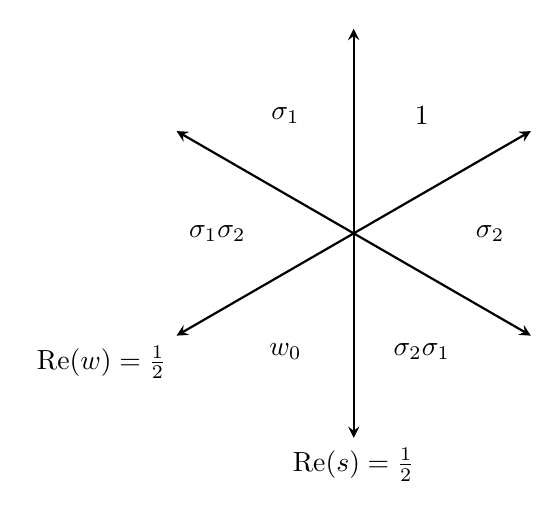
\begin{tikzpicture}[scale=3]
            \draw[thick,-stealth] (0:0) to (30:{sqrt(3)/2});
            \draw[thick,-stealth] (0:0) to (30:{-sqrt(3)/2}) node [below left] {$\Re(w) = \frac{1}{2}$};
            \draw[thick,-stealth] (0:0) to (90:{sqrt(3)/2});
            \draw[thick,-stealth] (0:0) to (90:{-sqrt(3)/2}) node [below] {$\Re(s) = \frac{1}{2}$};
            \draw[thick,-stealth] (0:0) to (150:{sqrt(3)/2});
            \draw[thick,-stealth] (0:0) to (150:{-sqrt(3)/2});

            \node at (60:{sqrt(3)/3}) {$1$};
            \node at (120:{sqrt(3)/3}) {$\s_{1}$};
            \node at (180:{sqrt(3)/3}) {$\s_{1}\s_{2}$};
            \node at (240:{sqrt(3)/3}) {$w_{0}$};
            \node at (300:{sqrt(3)/3}) {$\s_{2}\s_{1}$};
            \node at (0:{sqrt(3)/3}) {$\s_{2}$};
        \end{tikzpicture}
    \end{center}

    In the diagram, we have shifted the $(s,w)$-plane so that the origin lies at $\left(\frac{1}{2},\frac{1}{2}\right)$ and we have tiled the $(s,w)$-axes so that they are no longer perpendicular. The effect of these adjustments is that $\s_{1}$ and $\s_{2}$ act by rigid motions sending the region enclosing $1$ (corresponding to the identity) to either of the adjacent triangles. The other regions are obtained by acting by the corresponding element of $W$. The initial region $\L$ that $Z(s,w)$ is defined on is displayed in the figure below:
    
    \begin{center}
        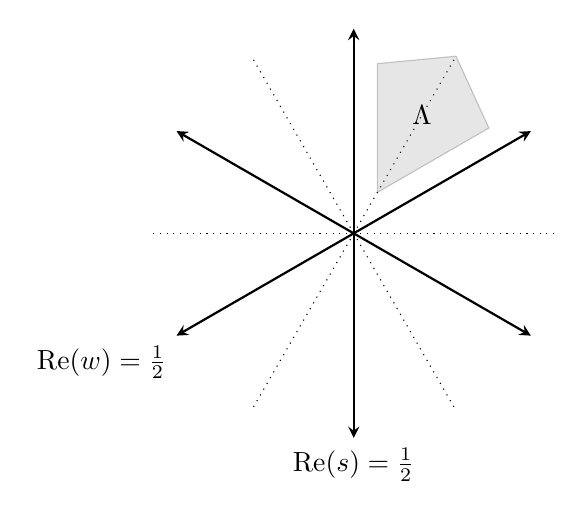
\begin{tikzpicture}[scale=3]
            \draw[dotted](0,0) to (60:{sqrt(3)/2});
            \draw[dotted](0,0) to (240:{sqrt(3)/2});
            \draw[dotted](0,0) to (180:{sqrt(3)/2});
            \draw[dotted](0,0) to (360:{sqrt(3)/2});
            \draw[dotted] (0:0) to (120:{sqrt(3)/2});
            \draw[dotted] (0:0) to (300:{sqrt(3)/2});

            \draw[thick,-stealth] (0:0) to (30:{sqrt(3)/2});
            \draw[thick,-stealth] (0:0) to (30:{-sqrt(3)/2}) node [below left] {$\Re(w) = \frac{1}{2}$};
            \draw[thick,-stealth] (0:0) to (90:{sqrt(3)/2});
            \draw[thick,-stealth] (0:0) to (90:{-sqrt(3)/2}) node [below] {$\Re(s) = \frac{1}{2}$};
            \draw[thick,-stealth] (0:0) to (150:{sqrt(3)/2});
            \draw[thick,-stealth] (0:0) to (150:{-sqrt(3)/2});


            \draw[fill=gray,opacity=0.2] (60:0.2) --+ (0,{((sqrt(5)/3)-0.2)}) -- (60:{sqrt(3)/2}) -- ($(60:0.2)+(30:{((sqrt(5)/3)-0.2)})$) -- cycle;

            \node at (60:{sqrt(3)/3}) {$\L$};
        \end{tikzpicture}
    \end{center}
    
     To meromorphically continue $Z(s,w)$ to all of the $(s,w)$-plane, we first need to show that the quadratic double Dirichlet series $Z(s,w)$ and $Z_{1,\t}(s,w)$ are locally absolutely uniformly convergent on a slightly larger region than $\L$. This will be achieved by the Phragm\'en-Lindel\"of convexity principal. Fix some small $\e > 0$. The functional equations for $L^{\ast}(s,\chi_{a_{1}d})$ and $L^{\ast}(w,\chi_{a_{2}m})$ provide the estimates
    \[
        L(-\e,\chi_{a_{1}d}) \ll |d|^{\frac{1}{2}+\e} \quad \text{and} \quad L(-\e,\chi_{a_{2}m}) \ll |m|^{\frac{1}{2}+\e},
    \]
    because $L(1+\e,\chi_{a_{1}d}) \ll 1$ and $L(1+\e,\chi_{a_{2}m}) \ll 1$. Since both of these $L$-functions have at most a simple pole at $s = 1$ and $w = 1$ respectively, the Phragm\'en-Lindel\"of convexity principal implies the weak estimates
    \[
        (s-1)L(s,\chi_{a_{1}d}) \ll |d|^{\frac{1}{2}+\e} \quad \text{and} \quad (w-1)L(w,\chi_{a_{2}m}) \ll |m|^{\frac{1}{2}+\e},
    \]
    for $\Re(s) > -\e$ and $\Re(w) > -\e$. But then from the interchange we see that $(s-1)(w-1)Z(s,w)$ and $(s-1)(w-1)Z_{1,\t}(s,w)$ are locally absolutely uniformly convergent on the region
    \[
        \L_{0} = \L \cup \left\{(s,w) \in \C^{2}:\Re(s) > 0, \Re(w) > \frac{3}{2}\right\} \cup \left\{(s,w) \in \C^{2}:\Re(s) > \frac{3}{2}, \Re(w) > 0\right\}.
    \]
    
    \begin{center}
        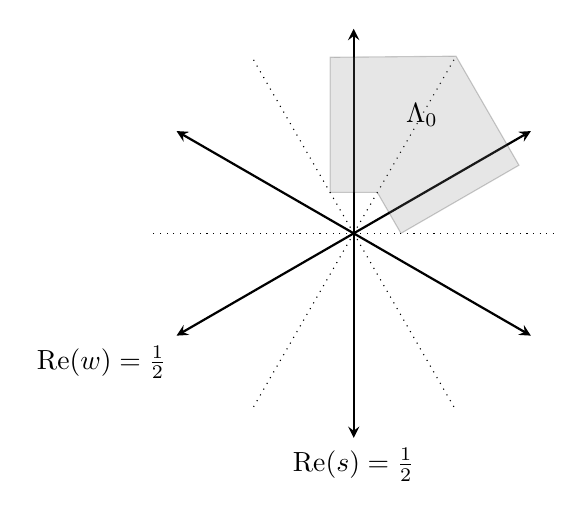
\begin{tikzpicture}[scale=3]
            \draw[dotted](0,0) to (60:{sqrt(3)/2});
            \draw[dotted](0,0) to (240:{sqrt(3)/2});
            \draw[dotted](0,0) to (180:{sqrt(3)/2});
            \draw[dotted](0,0) to (360:{sqrt(3)/2});
            \draw[dotted] (0:0) to (120:{sqrt(3)/2});
            \draw[dotted] (0:0) to (300:{sqrt(3)/2});

            \draw[thick,-stealth] (0:0) to (30:{sqrt(3)/2});
            \draw[thick,-stealth] (0:0) to (30:{-sqrt(3)/2}) node [below left] {$\Re(w) = \frac{1}{2}$};
            \draw[thick,-stealth] (0:0) to (90:{sqrt(3)/2});
            \draw[thick,-stealth] (0:0) to (90:{-sqrt(3)/2}) node [below] {$\Re(s) = \frac{1}{2}$};
            \draw[thick,-stealth] (0:0) to (150:{sqrt(3)/2});
            \draw[thick,-stealth] (0:0) to (150:{-sqrt(3)/2});

            \draw[fill=gray,opacity=0.2] (0:0.2) --+ (30:{cos(30)*((sqrt(3)/2)-0.2)}) -- (60:{sqrt(3)/2}) -- ($(120:0.2)+(0,{sqrt(5)/3-sin(120)*0.2})$) -- (120:0.2) -- (60:0.2) -- cycle;

            \node at (60:{sqrt(3)/3}) {$\L_{0}$};
        \end{tikzpicture}
    \end{center}
    
    In particular, $Z(s,w)$ and $Z_{1,\t}(s,w)$ are meromorphic on this region with at most polar lines at $s = 1$ and $w = 1$. The advantage of the region $\L_{0}$ over the intital region $\L$ is that $\L_{0}$ intersects the hyperplanes $s = \frac{1}{2}$ and $w = \frac{1}{2}$ so that the union of the reflections $w\L_{0}$ for $w \in W$ is connected. This guarantees that the functional equations imply meromorphic continuation since adjacent reflections of $\L_{0}$ overlap on open sets. The idea now is to reflect $\L_{0}$ via the functional equations and then apply a theorem of Bochner. To state this theorem we need a small definition. We say that a domain $\W \subset \C^{n}$ is a \textbf{tube domain} if there is an open set $\w \subset \R^{n}$ such that
    \[
        \W = \{(s_{1},\ldots,s_{n}) \in \C^{n}:\Re((s_{1},\ldots,s_{n})) \in \w\}.
    \]
    Tube domains are generalizations of vertical strips in the complex plane. Now we can state the theorem of Bochner (see \cite{hormander2000introduction} for a proof):

    \begin{theorem}[Bochner's continuation theorem]
        If $\W$ is a connected tube domain, then any holomorphic function on $\W$ can be extended to a holomorphic functon on the convex hull $\what{\W}$.
    \end{theorem}

    By clearing polar divisors, Bochner's continuation theorem implies that any meromorphic function on a connected tube domain posessing a finite amount of hyperplane polar divisors can be extended to a meromorphic function on the convex hull. This is exactly the situation for $Z(s,w)$. Indeed, it is clear that a union of tube domains is a tube domain and so, in particular, $\L_{0}$ is a tube domain. But on $\L_{0}$ there are a most polar lines at $s = 1$ and $w = 1$. Reflecting these hyperplanes via $W$ we obtain the finite set of possible polar divisors:
    \[
        \left\{s = 1, w = 1, s = 0, w = 0, s+w = \frac{1}{2}, s+w = \frac{3}{2}\right\}.
    \]
    Therefore we are reduced to extending $Z(s,w)$ meromorphically. By applying the functional equations corresponding to $\s_{1}$, $\s_{2}$, and $\s_{1}\s_{2}$, $Z(s,w)$ admits meromorphic continuation to the region
    \[
        \L_{12} = \L_{0} \cup \s_{1}\L_{0} \cup \s_{2}\L_{0} \cup \s_{1}\s_{2}\L_{0}.
    \]

    \begin{center}
        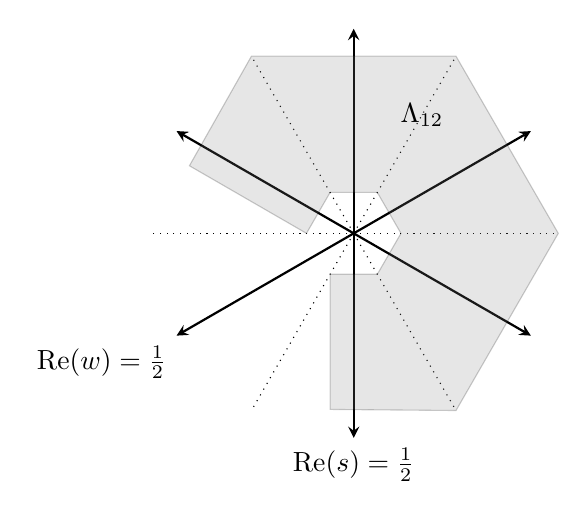
\begin{tikzpicture}[scale=3]
            \draw[dotted](0,0) to (60:{sqrt(3)/2});
            \draw[dotted](0,0) to (240:{sqrt(3)/2});
            \draw[dotted](0,0) to (180:{sqrt(3)/2});
            \draw[dotted](0,0) to (360:{sqrt(3)/2});
            \draw[dotted] (0:0) to (120:{sqrt(3)/2});
            \draw[dotted] (0:0) to (300:{sqrt(3)/2});

            \draw[thick,-stealth] (0:0) to (30:{sqrt(3)/2});
            \draw[thick,-stealth] (0:0) to (30:{-sqrt(3)/2}) node [below left] {$\Re(w) = \frac{1}{2}$};
            \draw[thick,-stealth] (0:0) to (90:{sqrt(3)/2});
            \draw[thick,-stealth] (0:0) to (90:{-sqrt(3)/2}) node [below] {$\Re(s) = \frac{1}{2}$};
            \draw[thick,-stealth] (0:0) to (150:{sqrt(3)/2});
            \draw[thick,-stealth] (0:0) to (150:{-sqrt(3)/2});

            \draw[fill=gray,opacity=0.2] (240:0.2) --+ (0,{-((sqrt(5)/3)+sin(240)*0.2)}) -- (300:{sqrt(3)/2}) -- (0:{sqrt(3)/2}) -- (60:{sqrt(3)/2}) -- (120:{sqrt(3)/2}) -- ($(180:0.2)+(150:{((sqrt(5)/3)+cos(150)*0.2)})$) -- (180:0.2) -- (120:0.2) -- (60:0.2) -- (0:0.2)-- (300:0.2) -- cycle;

            \node at (60:{sqrt(3)/3}) {$\L_{12}$};
        \end{tikzpicture}
    \end{center}

    Because the functional equations for $Z(s,w)$ involve both $Z(s,w)$ and $Z_{1,\t}(s,w)$, it was necessary to show that both of these quadratic double Dirichlet series were locally absolutely uniformly convergent on $\L_{0}$ before we applied the functional equation. Now $\L_{12}$ is a connected tube domain whose convex hull is $\C^{2}$. So by applying Bochner's continuation theorem (or rather our comment for meromorphic functions) we see that $Z(s,w)$ admits meromorphic continuation to the $(s,w)$-plane with at most a finite set of polar divisors. This method is better than repeatedly applying the functional equations corresponding to every $w \in W$. Indeed, if we did we would obtain meromorphic continuation to the region
    \[
        \L_{W} = \bigcup_{w \in W} w\L_{0}.
    \]

    \begin{center}
        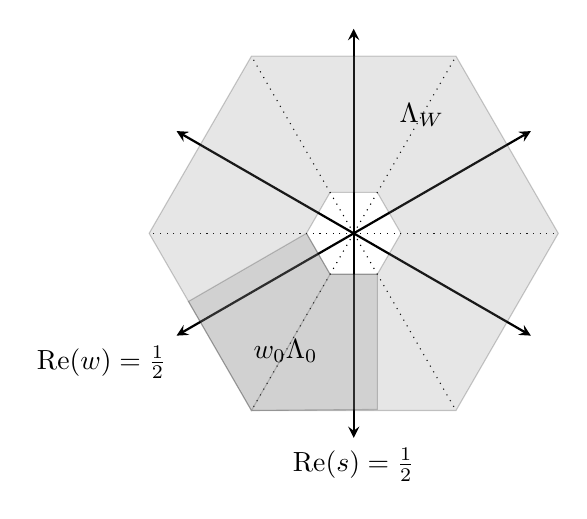
\begin{tikzpicture}[scale=3]
            \draw[dotted](0,0) to (60:{sqrt(3)/2});
            \draw[dotted](0,0) to (240:{sqrt(3)/2});
            \draw[dotted](0,0) to (180:{sqrt(3)/2});
            \draw[dotted](0,0) to (360:{sqrt(3)/2});
            \draw[dotted] (0:0) to (120:{sqrt(3)/2});
            \draw[dotted] (0:0) to (300:{sqrt(3)/2});

            \draw[thick,-stealth] (0:0) to (30:{sqrt(3)/2});
            \draw[thick,-stealth] (0:0) to (30:{-sqrt(3)/2}) node [below left] {$\Re(w) = \frac{1}{2}$};
            \draw[thick,-stealth] (0:0) to (90:{sqrt(3)/2});
            \draw[thick,-stealth] (0:0) to (90:{-sqrt(3)/2}) node [below] {$\Re(s) = \frac{1}{2}$};
            \draw[thick,-stealth] (0:0) to (150:{sqrt(3)/2});
            \draw[thick,-stealth] (0:0) to (150:{-sqrt(3)/2});
        
            \draw[fill=gray,opacity=0.2] (240:{sqrt(3)/2}) -- (300:{sqrt(3)/2}) -- (0:{sqrt(3)/2}) -- (60:{sqrt(3)/2}) -- (120:{sqrt(3)/2}) -- (180:{sqrt(3)/2}) -- (240:{sqrt(3)/2}) -- (240:0.2) -- (180:0.2) -- (120:0.2) -- (60:0.2) -- (0:0.2) -- (300:0.2) -- (240:0.2) -- cycle;

            \draw[fill=gray,opacity=0.2] (180:0.2) --+ (210:{-cos(210)*((sqrt(3)/2)-0.2)}) -- (240:{sqrt(3)/2}) -- ($(300:0.2)+(0,{-((sqrt(5)/3)+sin(300)*0.2)})$) -- (300:0.2) -- (240:0.2) -- cycle; 

            \node at (60:{sqrt(3)/3}) {$\L_{W}$};
            \node at (240:{sqrt(3)/3}) {$w_{0}\L_{0}$};
        \end{tikzpicture}
    \end{center}
    
    There are two issues here. The first is that $Z(s,w)$ has two meromorphic continuations to the region $w_{0}\L_{0}$ given by the functional equations corresponding to $w_{0} = \s_{1}\s_{2}\s_{1}$ and $w_{0} = \s_{2}\s_{1}\s_{2}$ and we would need to show that these agree. The second is that we have not obtained meromorphic continuation to $\C^{2}-\L_{W}$ which is a compact hexagon about the origin. By using Bochner's theorem after meromorphically continuning to $\L_{12}$, we have avoided these issues and as a consquence shown that the meromorphic continuations given by $w_{0} = \s_{1}\s_{2}\s_{1}$ and $w_{0} = \s_{2}\s_{1}\s_{2}$ agree.
\section{Poles and Residues}
    We will inespect the polar divisors of $Z(s,w)$ more carefully. It turns out that the set of polar divisors is smaller than
    \[
        \left\{s = 1, w = 1, s = 0, w = 0, s+w = \frac{1}{2}, s+w = \frac{3}{2}\right\}.
    \]
    Indeed, there are no poles on the hyperplanes $s = 0$, $w = 0$, and $s+w = \frac{3}{2}$. To see this, first note that by our earlier application of the Phragm\'en-Lindel\"of convexity principal we actually obtained continuation to an open set containing $\L_{0}$ (because our estimates held for $\Re(s) > -\e$ and $\Re(w) > -\e$). We did not need this larger region for the meromorphic continuation but we do need it to study the poles. Now consider the possible polar divisor $s = 0$. We know $(s-1)(w-1)Z(s,w)$ and $(s-1)(w-1)Z_{1,\t}(s,w)$ are holomorphic on an open set containing $\L_{0}$ which contains half of the hyperplane defined by $s = 0$ outside of the hexagon $\C^{2}-\L_{W}$. As $(s-1)(w-1)$ is holomorphic on this region it follows that $Z(s,w)$ and $Z_{1,\t}(s,w)$ do not have a polar divisor at $s = 0$ on an open set containing $\L_{0}$. Now note that an open set containing $\s_{1}\s_{2}\L_{0}$ contains the other half of the hyperplane defined by $s = 0$ outside of the hexagon $\C^{2}-\L_{W}$. Upon applying the functional equation corresponding to $\s_{1}\s_{2}$, \cref{FFthm:double_Dirichlet_series_functional_equation} implies that the gamma factors in the corresponding functional equation have a simple pole when $s+w = \frac{3}{2}$ (the gamma factors in the functional equation for $\s_{1}$ have a simple pole at $s = 1$ and $s-1 \to s+w-\frac{3}{2}$ under $\s_{2}$). Therefore $Z(s,w)$ and $Z_{1,\t}(s,w)$ do not have polar divisors at $s = 0$ on an open set containing $\s_{1}\s_{2}\L_{0}$ away from $s+w = \frac{3}{2}$. In particular, $Z(s,w)$ does not have a polar divisor at $s = 0$ on $\L_{W}$ and away from the other polar divisors. By Bochner's continuation theorem (after clearing all of the other possible polar divisors), we see that $Z(s,w)$ does not have a polar divisors at $s = 0$ on all of $\C^{2}$ and away from the other polar divisors. An identical argument holds for the case $w = 0$ with the regions $\L_{0}$ and $\s_{2}\s_{1}\L_{0}$. For the polar divisor $s+w = \frac{1}{2}$, we argue in the same way with the regions $\s_{2}\s_{1}\L_{0}$, $\s_{1}\s_{2}\L_{0}$, and $w_{0}\L_{0}$. The only difference is that for these regions the gamma factors in the corresponding functional equations are different. For the first two regions $\s_{2}\s_{1}\L_{0}$ and $\s_{1}\s_{2}\L_{0}$, the gamma factors have a simple pole when $s+w = \frac{3}{2}$. For the third region $w_{0}\L_{0}$, the gamma factors have simple poles at $s = 1$ and $w = 1$ which is seen by using both representations $w_{0} = \s_{1}\s_{2}\s_{1}$ and $w_{0} = \s_{2}\s_{1}\s_{2}$. So in conclusion, there are no poles on the hyperplanes $s = 0$, $w = 0$, and $s+w = \frac{1}{2}$ and away from the other polar divisors. As for the hyperplanes $s = 1$, $w = 1$, and $s+w = \frac{3}{2}$, there are clearly genuine poles for $s = 1$ and $w = 1$ coming from $L(s,\chi_{d_{0}})$ and $L(w,\chi_{m_{0}})$ when $d$ and $m$ are perfect squares (so that $d_{0} = m_{0} = 1$). For $s+w = \frac{3}{2}$, we have a pole coming from the gamma factors corresponding to the functional equations for $\s_{2}\s_{1}$ and $\s_{1}\s_{2}$. We collect all of our work as a theorem:

    \begin{theorem}
        $Z(s,w)$ admits meromorphic continuation to $\C^{2}$ with polar divisors $s = 1$, $w = 1$, and $s+w = \frac{3}{2}$.
    \end{theorem}

    We can now look at the residues of $Z(s,w)$ at these poles. Since all of the poles are obtained from each other by applying the functional equations of $Z(s,w)$, we begin by looking at the pole when $w = 1$. To compute the residue we use the representation
    \[
        Z(s,w) = \sum_{\text{$m$ monic}}\frac{L(w,\chi_{m_{0}})Q_{m_{0}m_{1}^{2}}(w)}{|m|^{s}},
    \]
    coming from the interchange. For a fixed $m$, the numerator $L(w,\chi_{m_{0}})Q_{m_{0}m_{1}^{2}}(w)$ in the summand has a pole at $w = 1$ if and only if $m_{0}$ is a perfect square, that is $m_{0} = 1$, or equivalently $m = m_{1}^{2}$ itself is a perfect square. In this case, $L(w,\chi_{m_{0}}) = \z(w)$ so that
    \[
        \Res_{w = 1}L(w,\chi_{m_{0}})Q_{m_{0}m_{1}^{2}}(w) = \frac{1}{\log(q)}Q_{m_{1}^{2}}(1).
    \]
    But from \cref{FFlem:prime_correction_even,FFthm:correction_polynomial_Euler_product} we see that $Q_{m_{1}^{2}}(1) = 1$, and so
    \[
        \Res_{w = 1}Z(s,w) = \frac{1}{\log(q)}\sum_{\text{$m$ monic perfect square}}\frac{Q_{m_{1}^{2}}(1)}{|m|^{s}} = \frac{1}{\log(q)}\sum_{\text{$m$ monic}}\frac{1}{|m|^{2s}} = \frac{1}{\log(q)}\z(2s).
    \]
    Notice that this expression has a simple pole at $s = \frac{1}{2}$ which is exactly when the polar lines $w = 1$ and $s+w = \frac{3}{2}$ intersect. The residue of $Z(s,w)$ at $s = 1$ is computed in an analogous way. Indeed, by applying the interchange, the exact same argument holds with the roles of $s$ and $w$ interchanged so that
    \[
        \Res_{s = 1}Z(s,w) = \frac{1}{\log(q)}\z(2w).
    \]
    Again, this expression has a simple pole at $w = \frac{1}{2}$ which is when the polar lines $s = 1$ and $s+w = \frac{3}{2}$ intersect. The other residues at the simple poles can be computed by applying the functional equations for $Z(s,w)$ and using the residues at $s = 1$ and $w = 1$. Now consider the point where the polar lines $w = 1$ and $s+w = \frac{3}{2}$ intersect. Setting $s = \frac{1}{2}$, we see that $Z\left(\frac{1}{2},w\right)$ has a pole at $w= 1$ and we would like to understand this pole better. To acomplish this, the Mittag-Leffler theorem applied to $Z(s,w)$ (in $w$) implies that
    \[
        Z(s,w) = \frac{R_{1}(s)}{w-1}+\frac{R_{2}(s)}{s+w-\frac{3}{2}}+V(s,w),
    \]
    in some neighborhood of $\left(\frac{1}{2},1\right)$, where $V(s,w)$ is holomorphic, and we have set
    \[
        R_{1}(s) = \Res_{w = 1}Z(s,w) \quad \text{and} \quad R_{2}(s) = \Res_{w = \frac{3}{2}-s}Z(s,w).
    \]
    From our residue computations, $R_{1}(s) = \frac{1}{\log(q)}\z(2s)$ which implies that it has a simple pole at $s = \frac{1}{2}$. The residue is given by $A = \frac{1}{2\log(q)}$. On the other hand, $Z\left(\frac{1}{2},w\right)$ is holomorphic for $\Re(w) > 1$. These two facts together imply that $R_{2}(s)$ must have a simple pole at $s = \frac{1}{2}$ which cancels the simple pole coming from $R_{1}(s)$. So by Mittag-Leffler again, we may write
    \[
        R_{1}(s) = \frac{A}{s-\frac{1}{2}}+R_{3}(s) \quad \text{and} \quad R_{2}(s) = -\frac{A}{s-\frac{1}{2}}+R_{4}(s),
    \]
    in a neighborhood of $s = \frac{1}{2}$ and where $R_{3}(s)$ and $R_{4}(s)$ are holomorphic. Then
    \begin{align*}
        Z(s,w) &= \frac{R_{1}(s)}{w-1}+\frac{R_{2}(s)}{s+w-\frac{3}{2}}+V(s,w) \\ 
        &= \frac{A}{(w-1)\left(s-\frac{1}{2}\right)}+\frac{R_{3}(s)}{w-1}-\frac{A}{\left(s+w-\frac{3}{2}\right)\left(s-\frac{1}{2}\right)}+\frac{R_{4}(s)}{s+w-\frac{3}{2}}+V(s,w) \\
        &= \frac{A}{(w-1)\left(s+w-\frac{3}{2}\right)}+\frac{R_{3}(s)}{w-1}+\frac{R_{4}(s)}{s+w-\frac{3}{2}}+V(s,w).
    \end{align*}
    We can now set $s = \frac{1}{2}$ and let $B = R_{3}\left(\frac{1}{2}\right)+R_{4}\left(\frac{1}{2}\right)$ so that
    \[
        Z\left(\frac{1}{2},w\right) = \frac{A}{(w-1)^{2}}+\frac{B}{w-1}+O(1).
    \]
    It follows that $Z\left(\frac{1}{2},w\right)$ has a double pole at $w = 1$. This can be thought of as follows: the polar lines $w = 1$ and $s+w = \frac{3}{2}$ correspond to simple poles of $Z(s,w)$ except in the case when they intersect and the order of the poles combine to give $Z\left(\frac{1}{2},w\right)$ a double pole at $w = 1$. Applying the interchange, the exact same argument holds to show that $Z\left(s,\frac{1}{2}\right)$ has a double pole at $s = 1$. We collect this work as a theorem:

    \begin{theorem}\label{FFthm:double_poles_at_1/2}
        $Z\left(\frac{1}{2},w\right)$ and $Z\left(s,\frac{1}{2}\right)$ have double poles at $w = 1$ and $s = 1$ respectively. In particular, in neighborhoods of $w = 1$ and $s = 1$ respectively, we have
        \[
            Z\left(\frac{1}{2},w\right) = \frac{A}{(w-1)^{2}}+\frac{B}{w-1}+O(1) \quad \text{and} \quad Z\left(s,\frac{1}{2}\right) = \frac{A}{(s-1)^{2}}+\frac{B}{s-1}+O(1),
        \]
        for some constants $A$ and $B$ with $A = \frac{1}{2\log(q)}$. 
    \end{theorem}
\section{An Application}
    As an application of the usefulness of quadratic double Dirichlet series, we show that the analytic properties of $Z(s,w)$ can be used to obtain a simultaneous non-vanishing result. In particular, we show that $L\left(\frac{1}{2},\chi_{d}\right)$ is nonzero for infinitely many $d$. Since the complex analysis involved comes from standard analytic number theory techniques, strictly speaking, we only sketch the result. To being, Perron's formula implies
    \[
        \sum_{\deg(d) \le X}L\left(\frac{1}{2},\chi_{d_{0}}\right)Q_{d_{0}d_{1}^{2}}\left(\frac{1}{2}\right) = \frac{1}{2\pi i}\int_{(2)}Z\left(\frac{1}{2},w\right)X^{w}\,dw,
    \]
    for some $X > 1$. It can be shown that $Z(s,w)$ is bounded in vertical strips provided we are away from poles. It follows that \cref{FFthm:double_poles_at_1/2} holds in vertical strips about the lines $\Re(w) = 1$ and $\Re(s) = 1$ respectively. Therefore
    \[
        \frac{1}{2\pi i}\int_{(2)}Z\left(\frac{1}{2},w\right)X^{w}\,dw = \frac{1}{2\pi i}\int_{(2)}\left(\frac{A}{(w-1)^{2}}+\frac{B}{w-1}+O(1)\right)X^{w}\,dw.
    \]
    Shifting the line of integration to the left (say to the line $\Re(w) = -2$) and using the residue theorem, we pick up a residue from the pole at $w = 1$. The contribution from the first two terms to the residue are $AX\log(X)$ and $BX$ respectively while the third term vanishes (recall that the integrand has a factor of $X^{w}$). The remaining vertical integral is $o(X)$. Therefore
    \[
        \frac{1}{2\pi i}\int_{(2)}Z\left(\frac{1}{2},w\right)X^{w}\,dw = AX\log(X)+BX+o(X),
    \]
    and it follows that
    \[
        \sum_{\deg(d) \le X}L\left(\frac{1}{2},\chi_{d_{0}}\right) = AX\log(X)+BX+o(X).
    \]
    But as $A = \frac{1}{2\log(q)} \neq 0$ (see \cref{FFthm:double_poles_at_1/2}) this means that $L\left(\frac{1}{2},\chi_{d}\right)$ must be nonzero for infinitely many $d$ (in particular for infinitely many square-free $d$). For otherwise, $\sum_{\deg(d) \le X}L\left(\frac{1}{2},\chi_{d_{0}}\right) = O(1)$ which gives a contradiction.
\section{\texorpdfstring{$Z(s,w)$}{Z(s,w)} as a Rational Function}
    Recall that $L(s,\chi_{d})$ is a polynomial in $q^{-s}$ of degree at most $\deg(d)-1$. A similar situation happens for the quadratic double Dirichlet series $Z(s,w)$, it will be a rational function in the variables $x = q^{-s}$ and $y = q^{-w}$. Since this property is a special case of Dirichlet series over function fields, we present the argument but supress the more detailed computations. Before we begin, we recall some properties of Hadamard products of power series. The details can be found in \cite{stanley2023enumerative}. For any two power series
    \[
        R_{1}(x,y) = \sum_{k,l \ge 0}r_{1}(k,l)x^{k}y^{l} \quad \text{and} \quad R_{2}(x,y) = \sum_{k,l \ge 0}r_{2}(k,l)x^{k}y^{l},
    \]
    or more generally generating series, their \textbf{Hadamard product} $(R_{1} \ast R_{2})(x,y)$ is defined by
    \[
        (R_{1} \ast R_{2})(x,y) = \sum_{k,l \ge 0}r_{1}(k,l)r_{2}(k,l)x^{k}y^{l}.
    \]
    If we assume $R_{1}(x,y)$ and $R_{2}(x,y)$ are regular around the origin $x = y = 0$, then the Hadamard product can be expressed as two contour integrals around the origin:
    \[
        (R_{1} \ast R_{2})(x,y) = \frac{1}{(2\pi i)^{2}}\int_{|z| = \rho}\int_{|w| = \rho}R_{1}(z,w)R_{2}\left(\frac{x}{z},\frac{y}{w}\right)\,\frac{dz}{z}\,\frac{dw}{w},
    \]
    for sufficiently small $\rho > 0$. By the residue theorem,
    \[
        (R_{1} \ast R_{2})(x,y) = \sum_{s = s(x,y)}\Res_{s}\left(\frac{R_{1}(z,w)R_{2}\left(\frac{x}{z},\frac{y}{w}\right)}{zw}\right),
    \]
    where the sum is over all poles $s = s(x,y)$ of the integrand such that $\lim_{x,y \to 0}s(x,y) = 0$. This formula can be used to compute the Hadamard product of rational functions. In the following argument where computing a Hadamard product is necessary, this method can be used.

    Now we show that $Z(s,w)$ is a rational function in $x = q^{-s}$ and $y = q^{-w}$. Throughout, we work in the region of local absolute uniform convergence for $Z(s,w)$. Consider the representation
    \[
        Z(s,w) = \sum_{\text{$d$ monic}}\frac{L(s,\chi_{d})}{|d|^{w}} = \sum_{\text{$m,d$ monic}}\frac{\chi_{d_{0}}(\what{m})a(m,d)}{|m|^{s}|d|^{w}}.
    \]
    Since $L(s,\chi_{d})$ is a polynomial in $q^{-s}$ of degree at most $\deg(d)-1$ and correction polynomials $Q_{d_{0}d_{1}^{2}}(s)$ are Dirichlet polynomials, one of the two following cases occur:
    \begin{itemize}
        \item If $d$ is a perfect square, then $L(s,\chi_{d_{0}}) = \z(s)$ and
        \[
            L(s,\chi_{d}) = \z(s)Q_{d_{1}^{2}}(s),
        \]
        where $Q_{d_{1}^{2}}(s)$ is a polynomial in $q^{-s}$ of degree $\deg(d)$.
        \item If $d$ is not a perfect square, then
        \[
            L(s,\chi_{d}) = L(s,\chi_{d_{0}})Q_{d_{0}d_{1}^{2}}(s),
        \]
        is a polynomial in $q^{-s}$ of degree at most $\deg(d)-1$.
    \end{itemize}
    So if $d$ is not a perfect square, then
    \[
        L(s,\chi_{d}) = \sum_{\deg(m) \le \deg(d)-1}\frac{\chi_{d_{0}}(\what{m})a(m,d)}{|m|^{s}},
    \]
    which is to say that
    \[
        \sum_{\deg(m) = k}\chi_{d_{0}}(\what{m})a(m,d) = 0,
    \]
    for every $k \ge \deg(d)$ provided $d$ is not a perfect square. To exploit this fact, we will decompose $Z(s,w)$ according to whether $\deg(d) \ge \deg(m)$ or $\deg(d) \le \deg(m)$. So we write
    \[
        Z(s,w) = Z_{0}(s,w)+Z_{0}(w,s)-Z_{1}(s,w),
    \]
    where
    \[
        Z_{0}(s,w) = \sum_{0 \le l \le k}\frac{1}{q^{ls}q^{kw}}\sum_{\substack{\text{$m,d$ monic} \\ \deg(m) = k \\ \deg(d) = l}}\chi_{d_{0}}(\what{m})a(m,d) \quad \text{and} \quad Z_{1}(s,w) = \sum_{k \ge 0}\frac{1}{q^{ks}q^{kw}}\sum_{\substack{\text{$m,d$ monic} \\ \deg(m) = k \\ \deg(d) = k}}\chi_{d_{0}}(\what{m})a(m,d).
    \]
    We will now show that $Z_{0}(s,w)$ and $Z_{1}(s,w)$ are rational functions in $q^{-s}$ and $q^{-w}$ via a convolution procedure. For $Z_{0}(s,w)$, our remarks about $L(s,\chi_{d})$ imply the term in the inner sum of $Z_{0}(s,w)$ vanishes unless $d$ is a perfect square and in this case $\chi_{d_{0}}(\what{m}) = 1$. Therefore
    \[
        Z_{0}(s,w) = \sum_{0 \le l \le k}\frac{1}{q^{ls}q^{kw}}\sum_{\substack{\text{$m,d$ monic} \\ \text{$d$ a perfect square} \\ \deg(m) = l \\ \deg(d) = k}}a(m,d).
    \]
    Now consider
    \[
        Y(s,w) = \sum_{\substack{\text{$m,d$ monic} \\ \text{$d$ monic perfect square}}}\frac{a(m,d)}{|m|^{s}|d|^{w}} \quad \text{and} \quad K_{0}(s,w) = \sum_{0 \le l \le k}\frac{1}{q^{ls}q^{kw}}.
    \]
    We can express both of these as rational functions in $q^{-s}$ and $q^{-w}$. Indeed, for $Y(s,w)$, \cref{FFprop:multiplicativity_of_weighting_coefficients}  we that $Y(s,w)$ posesses a Euler product. Using \cref{FFcor:evaulation_of_weighting_coefficients_at_primes}, we compute
    \[
        Y(s,w) = \frac{1-q^{1-s-2w}}{(1-q^{1-2w})(1-q^{1-s})(1-q^{2-2s-2w})},
    \]
    which can also be seen by comparing coefficients of the power series expansion of the right-hand side. $K_{0}(s,w)$ is even easier because it is a geometric series:
    \[
        K_{0}(s,w) = \sum_{0 \le l \le k}\frac{1}{q^{ls}q^{kw}} = \frac{1}{(1-q^{-s})(1-q^{-s-w})}.
    \]
    Then $Z_{0}(s,w)$ is expressed as a Hadamard product of power series in $q^{-s}$ and $q^{-w}$:
    \[
        Z_{0}(s,w) = Y(s,w) \ast K_{0}(s,w).
    \]
    Then using the countour integral representation of the Hadamard product, we compute
    \[
        Z_{0}(s,w) = \frac{1}{(1-q^{1-s})(1-q^{3-2s-2w})}.
    \]
    For $Z_{1}(s,w)$, our remarks about $L(s,\chi_{d})$ similarly imply
    \[
        Z_{1}(s,w) = \sum_{k \ge 0}\frac{1}{q^{ks}q^{kw}}\sum_{\substack{\text{$m,d$ monic} \\ \text{$d$ a perfect square} \\ \deg(m) = k \\ \deg(d) = k}}a(m,d).
    \]
    But then we may repeat the same argument as for $Z_{0}(s,w)$ with
    \[
        Y(s,w) = \sum_{\substack{\text{$m,d$ monic} \\ \text{$d$ monic perfect square}}}\frac{a(m,d)}{|m|^{s}|d|^{w}} \quad \text{and} \quad K_{1}(s,w) = \sum_{k \ge 0}\frac{1}{q^{ks}q^{kw}},
    \]
    and arrive at
    \[
        Z_{1}(s,w) = \frac{1}{(1-q^{3-2s-2w})}.
    \]
    Combining these representations for $Z_{0}(s,w)$ and $Z_{1}(s,w)$ with our decomposition of $Z(s,w)$ yields
    \[
        Z(s,w) = \frac{1-q^{2-s-w}}{(1-q^{1-s})(1-q^{1-w})(1-q^{3-2s-2w})}.
    \]
    Setting $x = q^{-s}$ and $y = q^{-w}$ gives
    \[
        Z(x,y) = \frac{1-q^{2}xy}{(1-qx)(1-qy)(1-q^{3}x^{2}y^{2})},
    \]
    which is a rational function in $x$ and $y$.

    \begin{remark}
        Some authors, especially those using the Chinta-Gunnells construction of building multiple Dirichlet series, prefer the $W$-invariant point to be at the origin. For this, we make the change of variables $\left(s+\frac{1}{2},w+\frac{1}{2}\right) \to (s,w)$ which gives
        \[
            Z(s,w) = \frac{1-q^{1-s-w}}{(1-q^{\frac{1}{2}-s})(1-q^{\frac{1}{2}-w})(2-q^{3-2s-2w})},
        \]
         and upon setting $x = q^{-s}$ and $y = q^{-w}$, we have
        \[
            Z(x,y) = \frac{1-qxy}{(1-q^{\frac{1}{2}}x)(1-q^{\frac{1}{2}}y)(1-q^{2}x^{2}y^{2})}.
        \]
    \end{remark}

\chapter{Quadratic Double Dirichlet Series II: The Number Field Case}
  \section{Preliminaries}
    We present an overview of quadratic Dirichlet $L$-functions over $\Q$. We begin with the Riemann zeta-function. The zeta function $\z(s)$ is defined as the Dirichlet series or Euler product
    \[
        \z(s) = \sum_{m \ge 1}\frac{1}{m^{s}} = \prod_{\text{$p$ prime}}\left(1-\frac{1}{p^{s}}\right)^{-1},
    \]
    for $\Re(s) > 1$. The second equality is an analytic reformulation of the fundamental theorem of arithmetic. The Riemann zeta function also admits meromorphic continuation to $\C$ with a simple pole at $s = 1$ of residue $1$. The functional equation is
    \[
        \pi^{-\frac{s}{2}}\G\left(\frac{s}{2}\right)\z(s) = \pi^{-\frac{1-s}{2}}\G\left(\frac{1-s}{2}\right)\z(1-s).
    \]
    Now we recall characters on $\Z$. They are multiplicative functions $\chi:\Z \to \C$ and form a group under multiplication. The two flavors we will care about are:
    
    \begin{itemize}
        \item Dirichlet characters: multiplicative functions $\chi_{d}:\Z \to \C$ modulo $d \ge 1$ (in that they are $d$-periodic) and such that $\chi_{d}(m) = 0$ if $(m,d) > 1$.
        \item Hilbert characters: The group of characters generated by those that appear in the sign change of reciprocity statements.
    \end{itemize}
    
    The image of a Dirichlet character always lands in the roots of unity. Moreover, $\conj{\chi}$ is the multiplicative inverse to $\chi$ and the Dirichlet characters modulo $d$ form a subgroup under multiplication. This group is always finite and its order is $\phi(d) = |(\F_{q}[t]/d\F_{q}[t])^{\x}|$. The Dirichlet characters that are of interest to us are those given by the quadratic residue symbol on $\Z$. First let us recall this symbol. For any odd prime $p$ and any $d \in \Z$, we define the quadratic residue symbol $\tlegendre{d}{p}$ by
    \[
        \legendre{d}{p} \equiv d^{\frac{p-1}{2}} \tmod{p} = \begin{cases} 1 & \text{if $x^{2} \equiv d \tmod{p}$ is solvable}, \\ -1 & \text{if $x^{2} \equiv d \tmod{p}$ is not solvable}, \\ 0 & \text{if $d \equiv 0 \tmod{p}$}. \end{cases}
    \]
    This symbol only depends upon $d$ modulo $p$ and is multiplicative in $d$. We can extend the quadratic residue symbol multiplicatively in the denominator. First we define
    \[
        \legendre{d}{-1} = \begin{cases} 1 & \text{if $d \ge 0$}, \\ -1 & \text{if $d < 0$}, \end{cases} \quad \text{and} \quad \legendre{d}{2} = \begin{cases} 1 & \text{if $d \equiv 1,7 \tmod{8}$}, \\ -1 & \text{if $d \equiv 3,5 \tmod{8}$}, \\ 0 & \text{if $d \equiv 0 \tmod{2}$}. \end{cases}
    \]
    If $m = up_{1}^{e_{1}}p_{2}^{e_{2}} \cdots p_{k}^{e_{k}}$ is the prime factorization of $m$ (with $u = \pm1$), then we define
    \[
        \legendre{d}{m} = \legendre{d}{u}\prod_{1 \le i \le k}\legendre{d}{p_{i}}^{e_{i}}.
    \]
    The quadratic residue symbol now makes sense for any $m \in \Z$ and is multiplicative in both $d$ and $m$. The quadratic residue symbol also admits the following reciprocity law:

    \begin{theorem}[Quadratic reciprocity]
        If $d,m \in \Z$, then
        \[
            \legendre{d}{m} = (-1)^{\frac{d^{(2)}-1}{2}\frac{m^{(2)}-1}{2}}\legendre{m}{|d|},
        \]
        where $d^{(2)}$ and $m^{(2)}$ are the parts of $d$ and $m$ relatively prime to $2$ respectively.
    \end{theorem}

    Moreover, we have the additional relations
    \[
        \legendre{-1}{m} = (-1)^{\frac{m^{(2)}-1}{2}} \quad \text{and} \quad \legendre{2}{m} = (-1)^{\frac{m^{2}-1}{8}},
    \]
    and if $m \not\equiv 0 \tmod{2}$, we can write
    \[
        \legendre{-1}{m} = (-1)^{\frac{m-1}{2}} = \begin{cases} 1 & \text{$m \equiv 1 \tmod{4}$}, \\ -1 & \text{$m \equiv 3 \tmod{4}$}, \end{cases} \quad \text{and} \quad \legendre{2}{m} = (-1)^{\frac{m^{2}-1}{8}} = \begin{cases} 1 & \text{$m \equiv 1,7 \tmod{8}$}, \\ -1 & \text{$m \equiv 3,5 \tmod{8}$}. \end{cases}
    \]

    We can now define the quadratic Dirichlet characters. For any square-free $d \in \Z$, define the quadratic Dirichlet character $\chi_{d}$ by the following quadratic residue symbol:
    \[
        \chi_{d}(m) = \begin{cases} \legendre{d}{m} & \text{if $d \equiv 1 \tmod{4}$}, \\ \legendre{4d}{m} & \text{if $d \equiv 2,3 \tmod{4}$}. \end{cases}
    \]
    This quadratic Dirichlet character is attached to the quadratic extension $\Q(\sqrt{d})$. We extend $\chi_{d}$ multiplicatively in the denominator so that $\chi_{d}$ makes sense for any odd $d$. In particular, $\chi_{d}(m) = \pm1$ provided $d$ and $m$ are relatively prime and $\chi_{d}(m) = 0$ if $(m,d) > 1$. Quadratic reciprocity implies that $\chi_{d}$ is a Dirichlet character modulo $|d|$ if $d \equiv 1 \tmod{4}$ and is a Dirichlet character modulo $|4d|$ if $d \equiv 2,3 \tmod{4}$. Indeed, if $d \equiv 1 \tmod{4}$ then $d^{(2)} = d$ and the sign is always $1$. If $d \equiv 3 \tmod{4}$, then $d^{(2)} = d$ and the sign is $\tlegendre{-1}{m}$ which is a character modulo $4$. If $d \equiv 2 \tmod{4}$, then $d^{(2)} \equiv 1,3 \tmod{4}$ and we are reduced to one of the previous two cases. We will also set
    \[
        q(d) = \begin{cases} |d| & \text{if $d \equiv 1 \tmod{4}$}, \\ |4d| & \text{if $d \equiv 2,3 \tmod{4}$}, \end{cases} \quad \text{and} \quad \e_{\chi_{d}} = \frac{\tau(\chi_{d})}{\sqrt{q(d)}} = \begin{cases} 1 & \text{if $d \equiv 1 \tmod{4}$}, \\ 1+i & \text{if $d \equiv 2,3 \tmod{4}$}, \end{cases}
    \]
    where $\tau(\chi_{d})$ is the Gauss sum attached to $\chi_{d}$. We will also require an associated character. For each $\chi_{m}$ (here we are purposely interchanging the roles of $d$ and $m$ to keep consistency with the notation when discussing the quadratic double Dirichlet series later), we define $\wtilde{\chi}_{m}$ by
    \[
        \wtilde{\chi}_{m}(d) = (-1)^{\frac{m^{(2)}-1}{2}\frac{d^{(2)}-1}{2}}\chi_{m}(|d|).
    \]
    By quadratic reciprocity, $\wtilde{\chi}_{m}$ is a quadratic Dirichlet character of the same modulus as $\chi_{m}$ and is multiplicative in $m$. Moreover, we have the identity $\wtilde{\wtilde{\chi}}_{m}(d) = \chi_{m}(|d|)$. Analogously, we set
    \[
        q(m) = \begin{cases} |m| & \text{if $m \equiv 1 \tmod{4}$}, \\ |4m| & \text{if $m \equiv 2,3 \tmod{4}$}, \end{cases} \quad \text{and} \quad \e_{\wtilde{\chi}_{m}} = \frac{\tau(\wtilde{\chi}_{m})}{\sqrt{q(m)}} = \begin{cases} 1 & \text{if $m \equiv 1 \tmod{4}$}, \\ 1+i & \text{if $m \equiv 2,3 \tmod{4}$}, \end{cases}
    \]
    where $\tau(\wtilde{\chi}_{m})$ is the Gauss sum attached to $\wtilde{\chi}_{m}$. We now discuss the Hilbert characters. We will only need four of them: the quadratic Dirichlet characters modulo $8$. They are given as follows:
    \begin{gather*}
        \chi_{1}(m) = \begin{cases} 1 &\text{if $m \not\equiv 0 \tmod{2}$}, \\ 0 &\text{if $m \equiv 0 \tmod{2}$}, \end{cases} \quad \chi_{-1}(m) = \begin{cases} 1 &\text{if $m \equiv 1 \tmod{4}$}, \\ -1 &\text{if $m \equiv 3 \tmod{4}$}, \\ 0 &\text{if $m \equiv 0 \tmod{2}$}, \end{cases} \\ \chi_{2}(m) = \begin{cases} 1 &\text{if $m \equiv 1,7 \tmod{8}$}, \\ -1 &\text{if $m \equiv 3,5 \tmod{8}$}, \\ 0 &\text{if $m \equiv 0 \tmod{2}$}, \end{cases} \quad \chi_{-2}(m) = \begin{cases} 1 &\text{if $m \equiv 1,3 \tmod{8}$}, \\ -1 &\text{if $m \equiv 5,7 \tmod{8}$}, \\ 0 &\text{if $m \equiv 0 \tmod{2}$}. \end{cases}
    \end{gather*}
    In general, we will denote a Hilbert character by $\chi_{a}$ with $a \in \{\pm1,\pm2\}$. The Hilbert characters also satisfy an important orthogonality property:

    \begin{theorem}[Orthogonality of Hilbert characters]
        If $d,m \in \Z$ are odd, then
        \[
            \frac{1}{4}\sum_{a \in \{\pm1,\pm2\}}\chi_{a}(dm) = \begin{cases} 1 & \text{if $d \equiv m \tmod{8}$}, \\ 0 & \text{if $d \not\equiv m \tmod{8}$}. \end{cases}
        \]
    \end{theorem}

    Also, we have the identities
    \[
        \wtilde{\chi}_{a}(m) = \chi_{a}(|m|), \quad \chi_{-1}(m) = \legendre{-1}{m}, \quad \text{and} \quad \chi_{2}(m) = \legendre{2}{m},
    \]
    and the relations
    \[
        \chi_{-2}(m) = \chi_{-1}(m)\chi_{2}(m), \quad \chi_{1}(m) = \chi_{-1}(m)\chi_{-1}(m), \quad \text{and} \quad \chi_{-1}(m) = \chi_{2}(m)\chi_{-2}(m).
    \]
    With the Dirichlet and Hilbert characters introduced, we are ready to discuss the $L$-functions associated to quadratic Dirichlet characters. We define the $L$-function $L(s,\chi_{d})$ attached to $\chi_{d}$ for square-free $d$, by a Dirichlet series or Euler product:
    \[
        L(s,\chi_{d}) = \sum_{m \ge 1}\frac{\chi_{d}(m)}{m^{s}} = \prod_{p \text{ prime}}\left(1-\frac{\chi_{d}(p)}{p^{s}}\right)^{-1}.
    \]
    By definition of the quadratic Dirichlet character, $L(s,\chi_{d}) \ll \z(s)$ for $\Re(s) > 1$ so that $L(s,\chi_{d})$ is locally absolutely uniformly convergent in this region. $L(s,\chi_{d})$ also admits analytic continuation to $\C$. The completed $L$-function $L^{\ast}(s,\chi_{d})$ is defined as
    \[
        L^{\ast}(s,\chi_{d}) = \begin{cases} \pi^{-\frac{s}{2}}\G\left(\frac{s}{2}\right)L(s,\chi_{d}) & \text{if $d > 0$}, \\ \pi^{-\frac{s}{2}}\G\left(\frac{s+1}{2}\right)L(s,\chi_{d}) & \text{if $d < 0$}. \end{cases}
    \]
    We have the functional equation
    \[
        L^{\ast}(s,\chi_{d}) = \e_{\chi_{d}}q(d)^{\frac{1}{2}-s}L^{\ast}(1-s,\chi_{d}),
    \]
    which can be equivalently expressed as
    \[
        L^{\ast}(s,\chi_{d}) = \begin{cases} |d|^{\frac{1}{2}-s}L^{\ast}(1-s,\chi_{d}) & \text{if $d \equiv 1,5 \tmod{8}$}, \\ (1+i)|4d|^{\frac{1}{2}-s}L^{\ast}(1-s,\chi_{d}) & \text{if $d \equiv 2,3,6,7 \tmod{8}$}. \end{cases}
    \]
    Note that the gamma factor depends upon $d$ modulo $8$. This the root cause of an important technical issue later when deriving functional equations for the quadratic double Dirichlet series. Analogously, the Dirichlet $L$-function $L(w,\wtilde{\chi}_{m})$ attached to $\wtilde{\chi}_{m}$ for square-free $m$ is defined by a Dirichlet series or Euler product:
    \[
        L(w,\wtilde{\chi}_{m}) = \sum_{d \ge 1}\frac{\wtilde{\chi}_{m}(d)}{d^{w}} = \prod_{p \text{ prime}}\left(1-\frac{\wtilde{\chi}_{m}(p)}{p^{w}}\right)^{-1}.
    \]
    As for $L(s,\chi_{d})$, $L(w,\wtilde{\chi}_{m}) \ll \z(w)$ for $\Re(w) > 1$ so that $L(w,\wtilde{\chi}_{m})$ is locally absolutely uniformly convergent in this region. Moreover, $L(w,\wtilde{\chi}_{m})$ admits analytic continuation to $\C$ and the completed $L$-function $L^{\ast}(w,\wtilde{\chi}_{m})$ is defined as
    \[
        L^{\ast}(w,\wtilde{\chi}_{m}) = \begin{cases} \pi^{-\frac{w}{2}}\G\left(\frac{w}{2}\right)L(w,\wtilde{\chi}_{m}) & \text{if $m \equiv 1,2,5 \tmod{8}$}, \\ \pi^{-\frac{w}{2}}\G\left(\frac{w+1}{2}\right)L(w,\wtilde{\chi}_{m}) & \text{if $m \equiv 3,6,7 \tmod{8}$}. \end{cases}
    \]
    We have the functional equation
    \[
        L^{\ast}(w,\wtilde{\chi}_{m}) = \e_{\wtilde{\chi}_{m}}q(m)^{\frac{1}{2}-w}L^{\ast}(1-w,\wtilde{\chi}_{m}),
    \]
    which can be equivalently expressed as
    \[
        L^{\ast}(w,\wtilde{\chi}_{m}) = \begin{cases} |m|^{\frac{1}{2}-w}L^{\ast}(1-w,\wtilde{\chi}_{m}) & \text{if $m \equiv 1,5 \tmod{8}$}, \\ (1+i)|4m|^{\frac{1}{2}-w}L^{\ast}(1-w,\wtilde{\chi}_{m}) & \text{if $m \equiv 2,3,6,7 \tmod{8}$}. \end{cases}
    \]
    Analogously, note that the gamma factor depends upon $m$ modulo $8$.

    \begin{remark}
        The definitions for $L(s,\chi_{d})$, $L^{\ast}(s,\chi_{d})$, $L(w,\wtilde{\chi}_{m})$, and $L^{\ast}(w,\wtilde{\chi}_{m})$ work perfectly well even when $d$ and $m$ are not square-free (however the functional equations do not hold). We purposely do not define these $L$-functions, yet, for $d$ and $m$ not necessarily square-free.
    \end{remark}
\section{The Quadratic Double Dirichlet Series}
    We will now define the quadratic double Dirichlet series $Z(s,w)$. For any integer $d \ge 1$, write $d = d_{0}d_{1}^{2}$ where $d_{0}$ is square-free. Equivalently, $d_{0}$ is the square-free part of $d$ and $\frac{d}{d_{0}}$ is a perfect square. The \textbf{quadratic double Dirichlet series} $Z(s,w)$ is defined as
    \[
        Z(s,w) = \sum_{\substack{d \ge 1 \\ (d,2) = 1}}\frac{L^{(2)}(s,\chi_{d_{0}})Q_{d_{0}d_{1}^{2}}(s)}{d^{w}},
    \]
    where $Q_{d_{0}d_{1}^{2}}(s)$ is the \textbf{correction polynomial} defined by
    \[
        Q_{d_{0}d_{1}^{2}}(s) = \sum_{e_{1}e_{2} \mid d_{1}}\mu(e_{1})\chi_{d_{0}}(e_{1})e_{1}^{-s}e_{2}^{1-s} = \sum_{e_{1}e_{2}e_{3} = d_{1}}\mu(e_{1})\chi_{d_{0}}(e_{1})e_{1}^{-s}e_{2}^{1-s},
    \]
    and $\mu$ is the usual M\"obius function. For $\Re(s) > 1$, there is the trivial estimate
    \[
        Q_{d_{0}d_{1}^{2}}(s) \ll \sum_{e_{1}e_{2} \mid d_{1}}1 \ll \s_{0}(d_{1})^{2} \ll_{\e} d_{1}^{2\e} \ll_{\e} d^{\e},
    \]
     for any $\e > 0$. As $L(s,\chi_{d_{0}}) \ll 1$ for $\Re(s) > 1$, $Z(s,w)$ is locally absolutely uniformly convergent in the region $\L = \{(s,w) \in \C^{2}:\Re(s) > 1, \Re(w) > 1\}$. It will also be necessary to consider quadratic double Dirichlet series twisted by a pair of Hilbert characters $\chi_{a_{1}}$ and $\chi_{a_{2}}$. The \textbf{quadratic double Dirichlet series} $Z_{a_{1},a_{2}}(s,w)$ twisted by $\chi_{a_{1}}$ and $\chi_{a_{2}}$ is defined as
    \[
        Z_{a_{1},a_{2}}(s,w) = \sum_{\substack{d \ge 1 \\ (d,2) = 1}}\frac{L^{(2)}(s,\chi_{a_{1}d_{0}})\chi_{a_{2}}(d)Q_{d_{0}d_{1}^{2}}(s,\chi_{a_{1}})}{d^{w}},
    \]
    where $Q_{d_{0}d_{1}^{2}}(s,\chi_{a_{1}})$ is the \textbf{correction polynomial} twisted by $\chi_{a_{1}}$ defined by
    \[
        Q_{d_{0}d_{1}^{2}}(s,\chi_{a_{1}}) = \sum_{e_{1}e_{2} \mid d_{1}}\mu(e_{1})\chi_{a_{1}d_{0}}(e_{1})e_{1}^{-s}e_{2}^{1-2s} = \sum_{e_{1}e_{2}e_{3} = d_{1}}\mu(e_{1})\chi_{a_{1}d_{0}}(e_{1})e_{1}^{-s}e_{2}^{1-2s},
    \]
    and $\mu$ is the usual M\"obius function. By definition of the Hilbert characters, we have the analogous bound $Q_{d_{0}d_{1}^{2}}(s,\chi_{a_{1}}) \ll d_{\e}$ so that $Z_{a_{1},a_{2}}(s,w)$ converges locally absolutely uniformly in the same region as $Z(s,w)$ does. In particular, $Z(s,w) = Z_{1,1}(s,w)$. We will also require quadratic double Dirichlet series correpsonding to the characters $\wtilde{\chi}_{m}$. Analogously writing $m = m_{0}m_{1}^{2}$, the \textbf{quadratic double Dirichlet series} $\wtilde{Z}(s,w)$ is defined as
    \[
        \wtilde{Z}(w,s) = \sum_{\substack{m \ge 1 \\ (m,2) = 1}}\frac{L^{(2)}(w,\wtilde{\chi}_{m_{0}})Q_{m_{0}m_{1}^{2}}(w)}{m^{s}},
    \]
    where $Q_{d_{0}d_{1}^{2}}(w)$ is the \textbf{correction polynomial} defined by
    \[
        Q_{m_{0}m_{1}^{2}}(w) = \sum_{e_{1}e_{2} \mid m_{1}}\mu(e_{1})\chi_{m_{0}}(e_{1})e_{1}^{-w}e_{2}^{1-w} = \sum_{e_{1}e_{2}e_{3} = m_{1}}\mu(e_{1})\chi_{m_{0}}(e_{1})e_{1}^{-w}e_{2}^{1-w},
    \]
    and $\mu$ is the usual M\"obius function. We have the analogous estimate $Q_{m_{0}m_{1}^{2}}(w) \ll_{\e} m^{\e}$ and as $L(w,\wtilde{\chi}_{m_{0}}) \ll 1$ for $\Re(w) > 1$, $\wtilde{Z}(w,s)$ is locally absolutely uniformly convergent in the same region as $Z(s,w)$. We also need to consider twists by a pair of Hilbert characters $\wtilde{\chi}_{a_{2}}$ and $\wtilde{\chi}_{a_{1}}$. The \textbf{quadratic double Dirichlet series} $\wtilde{Z}_{a_{2},a_{1}}(w,s)$ twisted by $\wtilde{\chi}_{a_{2}}$ and $\wtilde{\chi}_{a_{1}}$ is defined as
    \[
        \wtilde{Z}_{a_{2},a_{1}}(w,s) = \sum_{\substack{m \ge 1 \\ (m,2) = 1}}\frac{L^{(2)}(w,\wtilde{\chi}_{a_{2}m_{0}})\wtilde{\chi}_{a_{1}}(m)Q_{m_{0}m_{1}^{2}}(w,\wtilde{\chi}_{a_{2}})}{m^{s}},
    \]
    where $Q_{m_{0}m_{1}^{2}}(w,\wtilde{\chi}_{a_{2}})$ is the \textbf{correction polynomial} twisted by $\wtilde{\chi}_{a_{2}}$ defined by
    \[
        Q_{m_{0}m_{1}^{2}}(w,\wtilde{\chi}_{a_{2}}) = \sum_{e_{1}e_{2} \mid m_{1}}\mu(e_{1})\wtilde{\chi}_{a_{2}m_{0}}(e_{1})e_{1}^{-w}e_{2}^{1-2w} = \sum_{e_{1}e_{2}e_{3} = m_{1}}\mu(e_{1})\wtilde{\chi}_{a_{2}m_{0}}(e_{1})e_{1}^{-w}e_{2}^{1-2w}.
    \]
    and $\mu$ is the usual M\"obius function. By definition of the Hilbert characters, we have the analogous bound $Q_{m_{0}m_{1}^{2}}(w,\wtilde{\chi}_{a_{2}}) \ll_{\e} m^{\e}$ so that $\wtilde{Z}_{a_{2},a_{1}}(w,s)$ converges locally absolutely uniformly in the same region as $\wtilde{Z}(w,s)$ does. In particular, $\wtilde{Z}(w,s) = \wtilde{Z}_{1,1}(w,s)$.
\section{The Interchange}
    As defined, $Z_{a_{1},a_{2}}(s,w)$ is a sum of $L$-functions, and hence Euler products, in $s$. We will prove an interchange formula for $Z_{a_{1},a_{2}}(s,w)$ which will show that it can be expressed as a sum of $L$-functions in $w$. That is, we want the variables $s$ and $w$ to change places. Precisely:

    \begin{theorem}[Interchange]
        Wherever $Z_{a_{1},a_{2}}(s,w)$ converges locally absolutely uniformly,
        \[
            Z_{a_{1},a_{2}}(s,w) = \sum_{\substack{d \ge 1 \\ (d,2) = 1}}\frac{L^{(2)}(s,\chi_{a_{1}d_{0}})\chi_{a_{2}}(d)Q_{d_{0}d_{1}^{2}}(s,\chi_{a_{1}})}{d^{w}} = \sum_{\substack{m \ge 1 \\ (m,2) = 1}}\frac{L^{(2)}(w,\wtilde{\chi}_{a_{2}m_{0}})\wtilde{\chi}_{a_{1}}(m)Q_{m_{0}m_{1}^{2}}(w,\wtilde{\chi}_{a_{2}})}{m^{s}}.
        \]
        Moreover, the same holds for $\wtilde{Z}_{a_{2},a_{1}}(w,s)$.
    \end{theorem}
    \begin{proof}
        Only the second equality needs to be proved. To do this, first expand the $L$-function $L^{(2)}(s,\chi_{a_{1}d_{0}})$ and polynomial $Q_{d_{0}d_{1}^{2}}(s,\chi_{a_{1}})$ to get
        \begin{align*}
            Z(s,w) &= \sum_{\substack{d \ge 1 \\ (d,2) = 1}}\frac{L^{(2)}(s,\chi_{a_{1}d_{0}})\chi_{a_{2}}(d)Q_{d_{0}d_{1}^{2}}(s,\chi_{a_{1}})}{d^{w}} \\
            &= \sum_{\substack{d \ge 1 \\ (d,2) = 1}}\left(\sum_{\substack{m \ge 1 \\ (m,2) = 1}}\chi_{a_{1}d_{0}}(m)m^{-s}\right)\left(\sum_{e_{1}e_{2} \mid d_{1}}\mu(e_{1})\chi_{a_{1}d_{0}}(e_{1})e_{1}^{-s}e_{2}^{1-2s}\right)\chi_{a_{2}}(d)d^{-w} \\
            &= \sum_{\substack{d,m \ge 1 \\ (dm,2) = 1}}\sum_{e_{1}e_{2} \mid d_{1}}\mu(e_{1})\chi_{a_{2}}(d)\chi_{a_{1}d_{0}}(me_{1})e_{1}^{-s}e_{2}^{1-2s}m^{-s}d^{-w}.
        \end{align*}
        Now $\chi_{a_{1}d_{0}}(me_{1}) = 0$ unless $(d_{0},me_{1}) = 1$. We make this restriction on the sum giving
        \[
            \sum_{\substack{d,m \ge 1 \\ (dm,2) = 1}}\sum_{\substack{e_{1}e_{2} \mid d_{1} \\ (d_{0},me_{1}) = 1}}\mu(e_{1})\chi_{a_{2}}(d)\chi_{a_{1}d_{0}}(me_{1})e_{1}^{-s}e_{2}^{1-2s}m^{-s}d^{-w}.
        \]
        Making the change of variables $me_{1} \to m$ yields
        \[
            \sum_{\substack{d \ge 1 \\ (d,2) = 1}}\sum_{\substack{\substack{m \ge 1 \\ (m,2) = 1} \\ e_{1} \mid m}}\sum_{\substack{e_{1}e_{2} \mid d_{1} \\ (d_{0},m) = 1}}\mu(e_{1})\chi_{a_{2}}(d)\chi_{a_{1}d_{0}}(m)e_{2}^{1-2s}m^{-s}d^{-w}.
        \]
        For fixed $d = d_{0}d_{1}^{2}$ and $e_{2}$, the subsum over $m$ and $e_{1}$ is
        \[
            \sum_{\substack{\substack{m \ge 1 \\ (m,2) = 1} \\ e_{1} \mid m}}\sum_{\substack{e_{1} \mid \frac{d_{1}}{e_{2}} \\ (d_{0},m) = 1}}\mu(e_{1})\chi_{a_{1}d_{0}}(m)m^{-s} = \sum_{\substack{\substack{m \ge 1 \\ (m,2) = 1} \\ (d_{0},m) = 1}}\chi_{a_{1}d_{0}}(m)m^{-s}\left(\sum_{e_{1} \mid \left(\frac{d_{1}}{e_{2}},m\right)}\mu(e_{1})\right).
        \]
        The inner sum over $e_{1}$ of the M\"obius function vanishes unless $\left(\frac{d_{1}}{e_{2}},m\right) = 1$ in which case it is $1$. Therefore the triple sum above becomes
        \[
            \sum_{\substack{d,m \ge 1 \\ (dm,2) = 1}}\sum_{\substack{e_{2} \mid d_{1} \\ \left(\frac{d_{0}d_{1}}{e_{2}},m\right) = 1}}\chi_{a_{2}}(d)\chi_{a_{1}d_{0}}(m)e_{2}^{1-2s}m^{-s}d^{-w}.
        \]
        Making the change of variables $d \to de_{2}^{2}$, the condition $\left(\frac{d_{0}d_{1}}{e_{2}},m\right) = 1$ becomes $(d_{0}d_{1},m) = 1$ which is equivalent to $(d,m) = 1$. Moreover, $\chi_{a_{2}}(de_{2}^{2}) = \chi_{a_{2}}(d)$. Altogether, we obtain
        \[
            \sum_{\substack{\substack{d,m \ge 1 \\ (dm,2) = 1} \\ (d,m) = 1}}\sum_{e_{2}}\chi_{a_{2}}(d)\chi_{a_{1}d_{0}}(m)e_{2}^{1-2s-2w}m^{-s}d^{-w}.
        \]
        Writing $m = m_{0}m_{1}^{2}$ analogously as for $d$, quadratic reciprocity and positivity of $m$ and $d$ together imply $\chi_{d_{0}}(m) = \wtilde{\chi}_{m}(d_{0}) = \wtilde{\chi}_{m_{0}}(d)$ where the last equality holds because $(d,m) = 1$ and both $d_{0}$ and $m_{0}$ differ from $d$ and $m$ respectively by perfect squares. As $\chi_{a_{1}}(m) = \wtilde{\chi}_{a_{1}}(m)$ and $\chi_{a_{2}}(d) = \wtilde{\chi}_{a_{2}}(d)$ (again we use the positivity of $m$ and $d$), the previous fact implies $\chi_{a_{2}}(d)\chi_{a_{1}d_{0}}(m) = \wtilde{\chi}_{a_{1}}(m)\wtilde{\chi}_{a_{2}m_{0}}(d)$ and so our expression becomes
        \[
            \sum_{\substack{\substack{d,m \ge 1 \\ (dm,2) = 1} \\ (d,m) = 1}}\sum_{e_{2}}\wtilde{\chi}_{a_{1}}(m)\wtilde{\chi}_{a_{2}m_{0}}(d)e_{2}^{1-2s-2w}m^{-s}d^{-w}.
        \]
        But now we can reverse the argument with the roles of $d$, $m$, $\chi_{a_{1}}$, and $\chi_{a_{2}}$ interchanged respectively, but with $\wtilde{\chi}_{a_{1}}$ and $\wtilde{\chi}_{a_{2}}$, to obtain
        \[
            Z(s,w) = \sum_{\substack{m \ge 1 \\ (m,2) = 1}}\frac{L^{(2)}(w,\wtilde{\chi}_{a_{2}m_{0}})\wtilde{\chi}_{a_{1}}(m)Q_{m_{0}m_{1}^{2}}(w,\wtilde{\chi}_{a_{2}})}{m^{s}}.
        \]
        Clearly the same holds for $\wtilde{Z}_{a_{2},a_{1}}(w,s)$.
    \end{proof}

    Note that the interchange is not completely symmetric because of the characters $\wtilde{\chi}_{a_{2}m_{0}}$, $\wtilde{\chi}_{a_{1}}$, and $\wtilde{\chi}_{a_{2}}$ in the second expression for $Z_{a_{1},a_{2}}(s,w)$. This is due to the fact that reciprocity is not perfect. In even more general settings the correction polynomials in $w$ need not be equal to those in $s$.

    \begin{remark}\label{nf:rem:symmetry_of_Double_Dirichlet_series}
        When $a_{1} = a_{2} = 1$, the interchange implies
        \[
            Z(s,w) = \wtilde{Z}(w,s).
        \]
        More generally, the interchange implies the following relations for twisted quadratic double Dirichlet series:
        \[
            Z_{a_{1},a_{2}}(s,w) = \wtilde{Z}_{a_{2},a_{1}}(w,s),
        \]
        for $a_{1},a_{2} \in \{\pm1,\pm2\}$.
    \end{remark}
\section{Weighting Terms}
    We will now study the coefficients of $Z_{a_{1},a_{2}}(s,w)$ expanded in $s$ and $w$. Expanding $L^{(2)}(s,\chi_{a_{1}d_{0}})Q_{d_{0}d_{1}^{2}}(s,\chi_{a_{1}})$ in the numerator of $Z_{a_{1},a_{2}}(s,w)$, we can write
    \[
        Z_{a_{1},a_{2}}(s,w) = \sum_{\substack{d \ge 1 \\ (d,2) = 1}}\frac{L^{(2)}(s,\chi_{a_{1}d_{0}})\chi_{a_{2}}(d)Q_{d_{0}d_{1}^{2}}(s,\chi_{a_{1}})}{d^{w}} = \sum_{\substack{d,m \ge 1 \\ (dm,2) = 1}}\frac{\chi_{a_{1}d_{0}}(\what{m})\chi_{a_{2}}(d)H(m,d)}{m^{s}d^{w}},
    \]
    where $\what{m}$ is the part of $m$ relatively prime to $d_{0}$ and the \textbf{weighting coefficient} $H(m,d)$ is given by
    \[
        H(m,d) = \sum_{\substack{e_{1}e_{2}^{2}e_{3} = m \\ e_{1}e_{2} \mid d_{1} \\ (d_{0},e_{1}e_{3}) = 1}}\mu(e_{1})e_{2}.
    \]
    To see this, the coefficient of $m^{-s}d^{-w}$ in the definition of $Z_{a_{1},a_{2}}(s,w)$ is
    \begin{align*}
        \chi_{a_{2}}(d)\sum_{\substack{e_{1}e_{2}^{2}e_{3} = m \\ e_{1}e_{2} \mid d_{1}}}\mu(e_{1})\chi_{a_{1}d_{0}}(e_{1}e_{3})e_{2} &= \chi_{a_{2}}(d)\sum_{\substack{e_{1}e_{2}^{2}e_{3} = m \\ e_{1}e_{2} \mid d_{1} \\ (d_{0},e_{1}e_{3}) = 1}}\mu(e_{1})\chi_{a_{1}d_{0}}(e_{1}e_{3})e_{2} \\
        &= \chi_{a_{1}d_{0}}(\what{m})\chi_{a_{2}}(d)\sum_{\substack{e_{1}e_{2}^{2}e_{3} = m \\ e_{1}e_{2} \mid d_{1} \\ (d_{0},e_{1}e_{3}) = 1}}\mu(e_{1})e_{2} \\
        &= \chi_{a_{1}d_{0}}(\what{m})\chi_{a_{2}}(d)H(m,d),
    \end{align*}
    where the first equality holds because $\chi_{d_{0}}(e_{1}e_{3}) = 0$ unless $(d_{0},e_{1}e_{3}) = 1$ and the second equality holds because if $(d_{0},e_{1}e_{3}) = 1$, $\what{m}$ differs from $e_{1}e_{3}$ by a perfect square (the divisors of which belong to $(d_{0},e_{2})$) and so $\chi_{d_{0}}(e_{1}e_{3}) = \chi_{d_{0}}(\what{m})$. For completeness, we extend the definition of $H(m,d)$ to all $d,m \ge 1$. In particular, $H(m,d)$ makes sense when $m$ or $d$ may be even.
    
    \begin{remark}\label{nf:rem:weighting_coefficient_remark}
        Also, $H(m,d) = 0$ unless $m = e_{1}e_{2}^{2}e_{3}$ with $(d_{0},e_{1}e_{3}) = 1$ and $e_{1}e_{2}^{2} \mid d_{1}$.
    \end{remark}

    We will define $L(s,\chi_{a_{1}d})$ to be the Dirichlet series given by
    \[
        L(s,\chi_{a_{1}d}) = L(s,\chi_{a_{1}d_{0}})Q_{d_{0}d_{1}^{2}}(s,\chi_{a_{1}}) = \sum_{m \ge 1}\frac{\chi_{a_{1}d_{0}}(\what{m})H(m,d)}{m^{s}}.
    \]
    Clearly $L(s,\chi_{a_{1}d})$ is locally absolutely uniformly convergent for $\Re(s) > 1$. In particular, $L(s,\chi_{d})$ now makes sense for $d$ not necessarily square-free and this definition agrees with the former when $d$ is square-free. Moreover, we have the representation
    \[
        Z_{a_{1},a_{2}}(s,w) = \sum_{\substack{d \ge 1 \\ (d,2) = 1}}\frac{\chi_{a_{2}}(d)L^{(2)}(s,\chi_{a_{1}d})}{d^{w}}.
    \]
    If we perform the same procedure but with the interchange, we get
    \[
        \wtilde{Z}_{a_{2},a_{1}}(w,s) = \sum_{\substack{m \ge 1 \\ (m,2) = 1}}\frac{L^{(2)}(w,\wtilde{\chi}_{a_{2}m_{0}})\wtilde{\chi}_{a_{1}}(m)Q_{m_{0}m_{1}^{2}}(w,\wtilde{\chi}_{a_{2}})}{m^{s}} = \sum_{\substack{d,m \ge 1 \\ (dm,2) = 1}}\frac{\wtilde{\chi}_{a_{2}m_{0}}(\what{d})\wtilde{\chi}_{a_{1}}(m)H(d,m)}{m^{s}d^{w}},
    \]
    where $\what{d}$ is the part of $d$ relatively prime to $m_{0}$. Analogously, we define $L(w,\wtilde{\chi}_{a_{2}m})$ to be the Dirichlet series given by
    \[
        L(w,\wtilde{\chi}_{a_{2}m}) = L(w,\wtilde{\chi}_{a_{2}m_{0}})Q_{m_{0}m_{1}^{2}}(w,\wtilde{\chi}_{a_{2}}) = \sum_{d \ge 1}\frac{\wtilde{\chi}_{a_{2}m_{0}}(\what{d})H(d,m)}{d^{w}}.
    \]
    Again, $L(w,\wtilde{\chi}_{a_{2}m})$ is locally absolutely uniformly convergent for $\Re(w) > 1$. We also have
    \[
        \wtilde{Z}_{a_{2},a_{1}}(w,s) = \sum_{\substack{m \ge 1 \\ (m,2) = 1}}\frac{\wtilde{\chi}_{a_{1}}(m)L^{(2)}(w,\wtilde{\chi}_{a_{2}m})}{m^{s}}.
    \]
    We now investigate the structure of the weighting coefficients $H(m,d)$. Their structure controls the majority of the information about both the quadratic double Dirichlet series and the correction polynomials. We first show that the weighting coefficients posess a multiplicativity property:

    \begin{proposition}\label{nf:prop:multiplicativity_of_weighting_coefficients}
        We have $H(m,1) = H(1,d) = 1$ and
        \[
            H(m,d) = \prod_{\substack{p^{\a} \mid\mid m \\ p^{\b} \mid\mid d}}H(p^{\a},p^{\b}).
        \]
    \end{proposition}
    \begin{proof}
        From the definition of the weighting coefficients, $H(m,1) = H(1,d) = 1$. We will prove multiplicativity in $m$ and then in $d$. Letting $m = m'p^{\a}$, we must show
        \[
            H(m,d) = H(m',d)H(p^{\a},d).
        \]
        To acomplish this, for $e_{1}e_{2}^{2}e_{3} = m$, let $e_{1} = c_{1}d_{1}$, $e_{2} = c_{2}d_{2}$, and $e_{3} = c_{3}d_{3}$ with $c_{1},c_{2},c_{3} \mid m'$ and $d_{1},d_{2},d_{3} \mid p^{\a}$. Because $(m',p^{\a}) = 1$, as $e_{1}e_{2}^{2}e_{3}$ runs over decompositions of $m$, $c_{1}c_{2}^{2}c_{3}$ and $d_{1}d_{2}^{2}d_{3}$ run over decompositions of $m'$ and $p^{\a}$ respectively. Moreover, as $e_{1}e_{2}$ runs over the divisors of $d_{1}$ so does $c_{1}d_{1}c_{2}d_{2}$. These facts combined with multiplicativity of the M\"obius function gives
        \begin{align*}
            H(m,d) &= \sum_{\substack{e_{1}e_{2}^{2}e_{3} = m \\ e_{1}e_{2} \mid d_{1} \\ (d_{0},e_{1}e_{3}) = 1}}\mu(e_{1})e_{2} \\
            &= \sum_{\substack{c_{1}c_{2}^{2}c_{3} = m' \\ d_{1}d_{2}^{2}d_{3} = p^{\b} \\ c_{1}d_{1}c_{2}d_{2} \mid d_{1} \\ (d_{0},c_{1}d_{1}c_{3}d_{3}) = 1}}\mu(c_{1})(d_{1})|c_{2}|d_{2} \\
            &= \left(\sum_{\substack{c_{1}c_{2}^{2}c_{3} = m' \\ c_{1}c_{2} \mid d_{1} \\ (d_{0},c_{1}c_{3}) = 1}}\mu(c_{1})|c_{2}|\right)\left(\sum_{\substack{d_{1}d_{2}^{2}d_{3} = p^{\a} \\ d_{1}d_{2} \mid d_{1} \\ (d_{0},d_{1}d_{3}) = 1}}\mu(d_{1})d_{2}\right) \\
            &= H(m',d)H(p^{\a},d),
        \end{align*}
        as desired. Now we prove multiplicativity in $d$. Since we have already proven multiplicativity in $m$, we may assume $m = p^{\a}$. Letting $d = d'p^{\b}$, we must show
        \[
            H(p^{\a},d) = H(p^{\a},p^{\b}).
        \]
        As $e_{1}e_{2}^{2}e_{3} = p^{\a}$, the $e_{i}$ are powers of $p$ for $1 \le i \le 3$. It follows that $e_{1}e_{2} \mid d_{1}$ is equivalent to $e_{1}e_{2} \mid p^{\b}$. Moreover, $(d_{0},e_{1}e_{2}) = 1$ is equivalent to $(1,e_{1}e_{2}) = 1$ or $(p,e_{1}e_{2}) = 1$ depending on of $\b$ is even or odd. These facts imply the desired identity.
    \end{proof}

    The correction polynomials $Q_{d_{0}d_{1}^{2}}(s,\chi_{a_{1}})$ are tightly connected to the weighting coefficients $H(m,d)$. In particular, $Q_{d_{0}d_{1}^{2}}(s,\chi_{a_{1}})$ is a Dirichlet polynomial whose coefficients are essentially given by the weighting coefficients. We first prove this relationship when $d$ is an odd prime power:

    \begin{lemma}\label{nf:lem:prime_correction_odd}
        For any prime $p$ and $\a \ge 1$, we have
        \[
            Q_{p^{2\a+1}}(s) = \sum_{k \le 2\a}\frac{H(p^{k},p^{2\a+1})}{p^{ks}}.
        \]
        Moreover, the same holds for $Q_{p^{2\a+1}}(w)$.
    \end{lemma}
    \begin{proof}
        Expanding the correction polynomial in $p^{-s}$ yields
        \[
            Q_{p^{2\a+1}}(s) = \sum_{e_{1}e_{2} \mid p^{\a}}\mu(e_{1})\chi_{p}(e_{1})e_{1}^{-s}e_{2}^{1-2s} = \sum_{k \le 2\a}\frac{H'(P^{k},p^{2\a+1})}{p^{ks}}.
        \]
        where
        \[
            H'(P^{k},p^{2\a+1}) = \sum_{e_{1}e_{2}^{2} = p^{k}}\mu(e_{1})\chi_{p}(e_{1})e_{2}.
        \]
        The proof will be finished if we can show $H'(P^{k},p^{2\a+1}) = H(p^{k},p^{2\a+1})$. To see this, first observe $\mu(e_{1})\chi_{p}(e_{1}) = 0$ unless $e_{1} = 1$ in which case it is $1$. So $H'(P^{k},p^{2\a+1}) = 0$ if $k$ is odd and $p^{\frac{k}{2}}$ if $k$ is even. Compactly stated,
        \[
            H'(P^{k},p^{2\a+1}) = \begin{cases} p^{\frac{k}{2}} & \text{if $k$ is even}, \\ 0 & \text{if $k$ is odd}. \end{cases}
        \]
        On the other hand, $k \le \a$ so that
        \[
            H(p^{k},p^{2\a+1}) = \sum_{\substack{e_{1}e_{2}^{2}e_{3} = p^{k} \\ e_{1}e_{2} \mid p^{\a} \\ (p,e_{1}e_{3}) = 1}}\mu(e_{1})e_{2} = \sum_{\substack{e_{1}e_{2}^{2} \mid p^{k} \\ (p,e_{1}e_{3}) = 1}}\mu(e_{1})e_{2} = \sum_{e_{2}^{2} = p^{k}}e_{2} =  \begin{cases} p^{\frac{k}{2}} & \text{if $k$ is even}, \\ 0 & \text{if $k$ is odd}. \end{cases}
        \]
        This finishes the proof. Clearly the same holds for $Q_{p^{2\a+1}}(w)$.
    \end{proof}

    There is an analogous statement when $d$ is an even prime power up to a square-free factor and relatively prime factor:
    
    \begin{lemma}\label{nf:lem:prime_correction_even}
        For any square-free integer $d_{0} \ge 1$, $a_{1} \in \{\pm1,\pm2\}$, prime $p$ not dividing $d_{0}$, and $\b \ge 1$, we have
        \[
            Q_{d_{0}p^{2\b}}(s,\chi_{a_{1}}) = (1-\chi_{a_{1}d_{0}}(p)p^{-s})\sum_{k \le 2\b}\frac{\chi_{a_{1}d_{0}}(p^{k})H(p^{k},p^{2\b})}{p^{ks}}.
        \]
        Moreover, the same holds for $Q_{m_{0}p^{2\b}}(w,\wtilde{\chi}_{a_{2}})$.
    \end{lemma}
    \begin{proof}
        Expand the correction polynomial in $p^{-s}$ to get
        \[
            Q_{d_{0}p^{2\b}}(s,\chi_{a_{1}}) = \sum_{e_{1}e_{2} \mid p^{\a}}\mu(e_{1})\chi_{a_{1}d_{0}}(e_{1})e_{1}^{-s}e_{2}^{1-2s} = \sum_{k \le 2\b}\frac{H'(P^{k},p^{2\b})}{p^{ks}}.
        \]
        where
        \[
            H'(P^{k},p^{2\b}) = \sum_{e_{1}e_{2}^{2} = p^{k}}\mu(e_{1})\chi_{a_{1}d_{0}}(e_{1})e_{2}.
        \]
        It suffices to show $H'(P^{k},p^{2\b}) = \chi_{a_{1}d_{0}}(p^{k})\left(H(p^{k},p^{2\b})-H(p^{k-1},p^{2\b})\right)$. On the one hand, $\mu(e_{1}) = 0$ unless $e_{1} = 1,p$ in which case $\mu(e_{1}) = \pm1$ accordingly. So
        \[
            H'(P^{k},p^{2\b}) = \sum_{e_{1}e_{2}^{2} = p^{k}}\mu(e_{1})\chi_{a_{1}d_{0}}(e_{1})e_{2} = \begin{cases} \chi_{a_{1}d_{0}}(p^{k})p^{\frac{k}{2}} & \text{if $k$ is even}, \\ -\chi_{a_{1}d_{0}}(p^{k})p^{\frac{k-1}{2}} & \text{if $k$ is odd}, \end{cases}
        \]
        where we have used the identity $\chi_{a_{1}d_{0}}(e_{1}) = \chi_{a_{1}d_{0}}(p^{k})$ which holds because this quadratic Dirichlet character only depends upon the parity of $k$. On the other hand, as in the proof of \cref{nf:lem:prime_correction_odd} 
        \[
            H(p^{k},p^{2\b}) = \begin{cases} p^{\frac{k}{2}} & \text{if $k$ is even}, \\ 0 & \text{if $k$ is odd}. \end{cases}
        \]
        But then
        \[
            \chi_{a_{1}d_{0}}(p^{k})\left(H(p^{k},p^{2\b})-H(p^{k-1},p^{2\b})\right) = \begin{cases} \chi_{a_{1}d_{0}}(p^{k})p^{\frac{k}{2}} & \text{if $k$ is even}, \\ -\chi_{a_{1}d_{0}}(p^{k})p^{\frac{k-1}{2}} & \text{if $k$ is odd}, \end{cases}
        \]
        which completes the proof. Clearly the same holds for $Q_{m_{0}p^{2\b}}(w,\wtilde{\chi}_{a_{2}})$.
    \end{proof}

    \cref{nf:lem:prime_correction_odd,nf:lem:prime_correction_even} together show that $Q_{d_{0}d_{1}^{2}}(s,\chi_{a_{1}})$ is a Dirichlet polynomial whose coefficients are essentially given by the weighting coefficients $H(m,d)$ when $d$ is an prime power. The proof of these lemmas also give the value of $H(p^{k},p^{l})$ and we collect this as a corollary:

    \begin{corollary}\label{nf:cor:evaulation_of_weighting_coefficients_at_primes}
        For any prime $p$,
        \[
            H(p^{k},p^{l}) = \begin{cases} \min\left(p^{\frac{k}{2}},p^{\frac{l}{2}}\right) & \text{if $\min(k,l)$ is even}, \\ 0 & \text{otherwise}. \end{cases}
        \]
    \end{corollary}

    If we combine \cref{nf:prop:multiplicativity_of_weighting_coefficients,nf:cor:evaulation_of_weighting_coefficients_at_primes} we can compute $H(m,d)$ in general:

    \begin{corollary}\label{nf:cor:evaulation_of_weighting_coefficients_in_general}
        For any integers $d,m \ge 1$,
        \[
            H(m,d) = \begin{cases} (m,d)^{\frac{1}{2}} & \text{if $(m,d)$ is a perfect square}, \\ 0 & \text{otherwise}. \end{cases}
         \]
    \end{corollary}
    
    As an immediate consquence of \cref{nf:cor:evaulation_of_weighting_coefficients_in_general}, $H(m,d)$ is symmetric in $m$ and $d$. As the weighting coefficients are multiplicative, $Q_{d_{0}d_{1}^{2}}(s,\chi_{a_{1}})$ will posess an Euler product. To state the Euler product explicitely, we write $d = d_{0}d_{1}^{2}d_{2}^{2}$ with $d_{0}$ square-free and, $d_{2}$ relatively prime to $d_{0}d_{1}$, and such that every prime divisor of $d_{1}$ divides $d_{0}$. In other words, $d_{0}$ is the square-free part of $d$, $d_{1}$ is the square part of $d$ whose prime factors divide $d$ to odd power, and $d_{2}$ is the square part of $d$ whose prime factors divide $d$ to even power. We have the following Euler product:

    \begin{theorem}\label{nf:thm:correction_polynomial_Euler_product}
        Let $d = d_{0}d_{1}^{2}d_{2}^{2}$ be the square decomposition of $d$ stratified by even and odd powers. Then for any $a_{1} \in \{\pm1,\pm2\}$,
        \[
            Q_{d_{0}d_{1}^{2}d_{2}^{2}}(s,\chi_{a_{1}}) = \prod_{p^{\a} \mid\mid d_{1}}Q_{p^{2\a+1}}(s) \cdot \prod_{p^{\b} \mid\mid d_{2}}Q_{d_{0}p^{2\b}}(s,\chi_{a_{1}}).
        \]
        Moreover, the same holds for $Q_{m_{0}m_{1}^{2}m_{2}^{2}}(w,\wtilde{\chi}
        _{a_{2}})$.
    \end{theorem}
    \begin{proof}
        Recall that
        \[
            L(s,\chi_{a_{1}d}) = L(s,\chi_{a_{1}d_{0}})Q_{d_{0}d_{1}^{2}d_{2}^{2}}(s,\chi_{a_{1}}) = \sum_{m \ge 1}\frac{\chi_{a_{1}d_{0}}(\what{m})H(m,d)}{m^{s}}.
        \]
        We will now derive an alterate expression for $L(s,\chi_{a_{1}d})$. By \cref{nf:prop:multiplicativity_of_weighting_coefficients}, the coefficients of $L(s,\chi_{a_{1}d})$ are multiplicative. Therefore $L(s,\chi_{a_{1}d})$ admits the Euler product
        \[
            L(s,\chi_{a_{1}d}) = \prod_{\text{$p$ prime}}\left(\sum_{k \ge 0}\frac{\chi_{a_{1}d_{0}}(\what{p^{k}})H(p^{k},d)}{p^{ks}}\right).
        \]
        Decomposing the product according to primes dividing $d = d_{0}d_{1}^{2}d_{2}^{2}$, we get
        \begin{align*}
            & L(s,\chi_{a_{1}d}) \\
            &= \prod_{\text{$p$ prime}}\left(\sum_{k \ge 0}\frac{\chi_{a_{1}d_{0}}(\what{p^{k}})H(p^{k},d)}{p^{ks}}\right) \\
            &= \prod_{p \nmid d}\left(\sum_{k \ge 0}\frac{\chi_{a_{1}d_{0}}(\what{p^{k}})H(p^{k},1)}{p^{ks}}\right)\prod_{p^{\a} \mid\mid d_{1}}\left(\sum_{k \ge 0}\frac{\chi_{a_{1}d_{0}}(\what{p^{k}})H(p^{k},p^{2\a+1})}{p^{ks}}\right) \cdot \prod_{p^{\b} \mid\mid d_{2}}\left(\sum_{k \ge 0}\frac{\chi_{a_{1}d_{0}}(\what{p^{k}})H(p^{k},p^{\b})}{p^{ks}}\right) \\
            &= \prod_{p \nmid d}\left(\sum_{k \ge 0}\frac{\chi_{a_{1}d_{0}}(\what{p^{k}})}{p^{ks}}\right)\prod_{p^{\a} \mid\mid d_{1}}\left(\sum_{k \ge 0}\frac{\chi_{a_{1}d_{0}}(\what{p^{k}})H(p^{k},p^{2\a+1})}{p^{ks}}\right) \cdot \prod_{p^{\b} \mid\mid d_{2}}\left(\sum_{k \ge 0}\frac{\chi_{a_{1}d_{0}}(\what{p^{k}})H(p^{k},p^{\b})}{p^{ks}}\right) \\
            &= \prod_{p \nmid d}\left(\sum_{k \ge 0}\frac{\chi_{a_{1}d_{0}}(\what{p^{k}})}{p^{ks}}\right)\prod_{p^{\a} \mid\mid d_{1}}\left(\sum_{k \ge 0}\frac{H(p^{k},p^{2\a+1})}{p^{ks}}\right) \cdot \prod_{p^{\b} \mid\mid d_{2}}\left(\sum_{k \ge 0}\frac{\chi_{a_{1}d_{0}}(p^{k})H(p^{k},p^{\b})}{p^{ks}}\right).
        \end{align*}
        Including the factors corresponding to primes $p \mid d_{2}$ into the first product, we must multiply the last factor by the inverse of $\sum_{k \ge 0}\chi_{a_{1}d_{0}}(p)p^{-ks} = (1-\chi_{a_{1}d_{0}}(p)p^{-s})^{-1}$ obtaining
        \[
            \prod_{p \nmid d_{0}}\left(\sum_{k \ge 0}\frac{\chi_{a_{1}d_{0}}(\what{p^{k}})}{p^{ks}}\right)\prod_{p^{\a} \mid\mid d_{1}}\left(\sum_{k \ge 0}\frac{H(p^{k},p^{2\a+1})}{p^{ks}}\right) \cdot \prod_{p^{\b} \mid\mid d_{2}}\left((1-\chi_{a_{1}d_{0}}(p)p^{-s})\sum_{k \ge 0}\frac{\chi_{a_{1}d_{0}}(p^{k})H(p^{k},p^{\b})}{p^{ks}}\right),
        \]
        as every prime divisor of $d_{1}$ divdes $d_{0}$. The first product is $L(s,\chi_{a_{1}d_{0}})$. For the second and third products, \cref{nf:rem:weighting_coefficient_remark} implies that the sums run up to $k \le 2\a$ and $k \le 2\b$ respectively. Therefore they are $Q_{p^{2\a+1}}(s)$ and $Q_{d_{0}p^{2\b}}(s,\chi_{a_{1}})$ respectively. It follows that
        \[
            L(s,\chi_{a_{1}d}) = L(s,\chi_{a_{1}d_{0}}) \cdot \prod_{p^{\a} \mid\mid d_{1}}Q_{p^{2\a+1}}(s) \cdot \prod_{p^{\b} \mid\mid d_{2}}Q_{d_{0}p^{2\b}}(s,\chi_{a_{1}}).
        \]
        This is our alternate expression for $L(s,\chi_{a_{1}d})$ and equating the two results in
        \[
            L(s,\chi_{a_{1}d_{0}})Q_{d_{0}d_{1}^{2}d_{2}^{2}}(s,\chi_{a_{1}}) = L(s,\chi_{a_{1}d_{0}}) \cdot \prod_{p^{\a} \mid\mid d_{1}}Q_{p^{2\a+1}}(s) \cdot \prod_{p^{\b} \mid\mid d_{2}}Q_{d_{0}p^{2\b}}(s,\chi_{a_{1}}),
        \]
        from which the proof is complete since $L(s,\chi_{a_{1}d_{0}}) \neq 0$ for $\Re(s) > 1$ (so that we may divide by $L(s,\chi_{a_{1}d_{0}})$). Clearly the same holds for $Q_{m_{0}m_{1}^{2}m_{2}^{2}}(w,\wtilde{\chi}_{a_{2}})$.
    \end{proof}

    Observe that for $d = d_{0}d_{1}^{2}d_{2}^{2}$, the prime factors that divide $d_{1}d_{2}$ are exactly those factors that divide $d$ to power larger than $1$. Thus, from \cref{nf:thm:correction_polynomial_Euler_product} the Euler product for $Q_{d_{0}d_{1}^{2}d_{2}^{2}}(s,\chi_{a_{1}})$ is supported on exactly the primes dividing $d$ to order larger than $1$ and also depends upon the character $\chi_{a_{1}d_{0}}$.
\section{Functional Equations}
    We can now derive functional equations for $Z_{a_{1},a_{2}}(s,w)$. These functional equations will be induced from the functional equations for $L(s,\chi_{a_{1}d})$ and $L(s,\wtilde{\chi}_{a_{2}m})$. To prove these latter functional equations, we require a functional equation for the correction polynomials:

    \begin{theorem}\label{nf:thm:functional_equation_correction_polynomials}
        $Q_{d_{0}d_{1}^{2}}(s,\chi_{a_{1}})$ admits the functional equation.
        \[
            Q_{d_{0}d_{1}^{2}}(s,\chi_{a_{1}}) = d_{1}^{1-2s}Q_{d_{0}d_{1}^{2}}(1-s,\chi_{a_{1}}).
        \]
        Moreover, the same holds for $Q_{m_{0}m_{1}^{2}}(w,\wtilde{\chi}_{a_{2}})$.
    \end{theorem}
    \begin{proof}
        The stragety is to interchange $e_{2}$ and $e_{3}$ in the sum defining $Q_{d_{0}d_{1}^{2}}(s,\chi_{a_{1}})$:
        \begin{align*}
            d_{1}^{1-2s}Q_{d_{0}d_{1}^{2}}(1-s) &= d_{1}^{1-2s}\sum_{e_{1}e_{2}e_{3} = d_{1}}\mu(e_{1})\chi_{a_{1}d_{0}}(e_{1})e_{1}^{s-1}e_{2}^{2s-1} \\
            &= \sum_{e_{1}e_{2}e_{3} = d_{1}}\mu(e_{1})\chi_{a_{1}d_{0}}(e_{1})e_{1}^{s-1}\left(\frac{d_{1}}{e_{2}}\right)^{1-2s} \\
            &= \sum_{e_{1}e_{2}e_{3} = d_{1}}\mu(e_{1})\chi_{a_{1}d_{0}}(e_{1})e_{1}^{s-1}(e_{1}e_{3})^{1-2s} \\
            &= \sum_{e_{1}e_{2}e_{3} = d_{1}}\mu(e_{1})\chi_{a_{1}d_{0}}(e_{1})e_{1}^{-s}e_{3}^{1-2s} \\
            &= Q_{d_{0}d_{1}^{2}}(s,\chi_{a_{1}}).
        \end{align*}
        Clearly the same holds for $Q_{m_{0}m_{1}^{2}}(w,\wtilde{\chi}_{a_{2}})$.
    \end{proof}

    We will define the completed $L$-function $L^{\ast}(s,\chi_{a_{1}d})$ by
    \[
        L^{\ast}(s,\chi_{a_{1}d}) = L^{\ast}(s,\chi_{a_{1}d_{0}})Q_{d_{0}d_{1}^{2}}(s,\chi_{a_{1}}).
    \]
    In particular, $L^{\ast}(s,\chi_{d})$ makes sense even when $d$ is not square-free and agrees with the previous definition when $d$ is square-free. Combining \cref{nf:thm:functional_equation_correction_polynomials}, the functional equation for $L^{\ast}(s,\chi_{a_{1}d_{0}})$, and that $d \equiv d_{0} \tmod{4}$, we obtain a functional equation for $L^{\ast}(s,\chi_{a_{1}d})$:
    \[
        L^{\ast}(s,\chi_{a_{1}d}) = \begin{cases} |d|^{\frac{1}{2}-s}L^{\ast}(1-s,\chi_{a_{1}d}) & \text{if $a_{1}d \equiv 1,5 \tmod{8}$}, \\ (1+i)|8d|^{\frac{1}{2}-s}L^{\ast}(1-s,\chi_{a_{1}d}) & \text{if $a_{1}d \equiv 2,3,6,7 \tmod{8}$}. \end{cases}
    \]
    Analogously, define the completed $L$-function $L^{\ast}(w,\wtilde{\chi}_{a_{2}m})$ by
    \[
        L^{\ast}(w,\wtilde{\chi}_{a_{2}m}) = L^{\ast}(w,\wtilde{\chi}_{a_{2}m_{0}})Q_{m_{0}m_{1}^{2}}(w,\wtilde{\chi}_{a_{2}}).
    \]
    Then, as before, we have a functional equation for $L^{\ast}(w,\wtilde{\chi}_{a_{2}m})$:
    \[
        L^{\ast}(w,\wtilde{\chi}_{a_{2}m}) = \begin{cases} |m|^{\frac{1}{2}-w}L^{\ast}(1-w,\wtilde{\chi}_{a_{2}m}) & \text{if $a_{2}m \equiv 1,5 \tmod{8}$}, \\ (1+i)|8m|^{\frac{1}{2}-w}L^{\ast}(1-w,\wtilde{\chi}_{a_{2}m}) & \text{if $a_{2}m \equiv 2,3,6,7 \tmod{8}$}. \end{cases}
    \]
    The functional equations for $L^{\ast}(s,\chi_{a_{1}d})$ and $L^{\ast}(w,\wtilde{\chi}_{a_{2}m})$ will induce functional equations for $Z_{a_{1},a_{2}}(s,w)$ and $\wtilde{Z}_{a_{2},a_{1}}(w,s)$. However, there is an obstruction caused by the gamma factors. Indeed, the gamma factors for $L^{\ast}(s,\chi_{a_{1}d})$ and $L^{\ast}(w,\wtilde{\chi}_{a_{2}m})$ depend $a_{1}d$ and $a_{2}m$ modulo $8$ respectively. To induce functional equations we need the gamma factors to be constant. Orthogonality of the Hilbert characters will allow us to get past this issue. For $b \in \{1,3,5,7\}$, define $Z_{a_{1},a_{2}}^{b}(s,w)$ and $\wtilde{Z}_{a_{2},a_{1}}^{b}(w,s)$ by
    \[
        Z_{a_{1},a_{2}}^{b}(s,w) = \frac{1}{4}\sum_{a \in \{\pm1,\pm2\}}\chi_{a}(b)Z_{a_{1},aa_{2}}(s,w) \quad \text{and} \quad \wtilde{Z}_{a_{2},a_{1}}^{b}(w,s) = \frac{1}{4}\sum_{a \in \{\pm1,\pm2\}}\wtilde{\chi}_{a}(b)\wtilde{Z}_{a_{2},aa_{1}}(w,s).
    \]
    In terms of the representations
    \[
        Z_{a_{1},a_{2}}(s,w) = \sum_{\substack{d \ge 1 \\ (d,2) = 1}}\frac{\chi_{a_{2}}(d)L^{(2)}(s,\chi_{a_{1}d})}{d^{w}} \quad \text{and} \quad \wtilde{Z}_{a_{2},a_{1}}(w,s) = \sum_{\substack{m \ge 1 \\ (m,2) = 1}}\frac{\wtilde{\chi}_{a_{1}}(m)L^{(2)}(w,\wtilde{\chi}_{a_{2}m})}{m^{s}},
    \]
    and orthogonality of the Hilbert characters, $Z_{a_{1},a_{2}}^{b}(s,w)$ and $\wtilde{Z}_{a_{2},a_{1}}^{b}(w,s)$ are the subseries containing only those $d$ and $m$ equivalent to $b$ modulo $8$ respectively. Then $Z_{a_{1},a_{2}}^{b}(s,w)$ and $\wtilde{Z}_{a_{2},a_{1}}^{b}(w,s)$ are sums of $L$-functions with a fixed gamma factor and so we can obtain functional equations. The fact that $Z_{a_{1},a_{2}}(s,w)$ and $\wtilde{Z}_{a_{2},a_{1}}(w,s)$ are linear combinations of these series will induce function equations. Precisely, we have the following statement:

    \begin{theorem}\label{nf:thm:double_Dirichlet_series_functional_equation}
        $Z_{a_{1},a_{2}}(s,w)$ admits the functional equations
        \begin{align*}
            Z_{a_{1},a_{2}}(s,w) &= \frac{1}{4}\pi^{s-\frac{1}{2}}\frac{\G\left(\frac{1-s}{2}\right)}{\G\left(\frac{s}{2}\right)}\sum_{\substack{a_{1}b > 0 \\ a_{1}b \equiv 1,5 \tmod{8} \\ a \in \{\pm1,\pm2\}}}\chi_{a}(b)\frac{(1-\chi_{a_{1}b}(2)2^{s-1})^{-1}}{(1-\chi_{a_{1}b}(2)2^{-s})^{-1}}Z_{a_{1},aa_{2}}\left(1-s,s+w-\frac{1}{2}\right) \\
            &+\frac{1}{4}\pi^{s-\frac{1}{2}}\frac{\G\left(\frac{-s}{2}\right)}{\G\left(\frac{s+1}{2}\right)}\sum_{\substack{a_{1}b < 0 \\ a_{1}b \equiv 1,5 \tmod{8} \\ a \in \{\pm1,\pm2\}}}\chi_{a}(b)\frac{(1-\chi_{a_{1}b}(2)2^{s-1})^{-1}}{(1-\chi_{a_{1}b}(2)2^{-s})^{-1}}Z_{a_{1},aa_{2}}\left(1-s,s+w-\frac{1}{2}\right) \\
            &+\frac{1+i}{8^{s}}\pi^{s-\frac{1}{2}}\frac{\G\left(\frac{1-s}{2}\right)}{\G\left(\frac{s}{2}\right)}\sum_{\substack{a_{1}b > 0 \\ a_{1}b \equiv 2,3,6,7 \tmod{8} \\ a \in \{\pm1,\pm2\}}}\chi_{a}(b)\frac{(1-\chi_{a_{1}b}(2)2^{s-1})^{-1}}{(1-\chi_{a_{1}b}(2)2^{-s})^{-1}}Z_{a_{1},aa_{2}}\left(1-s,s+w-\frac{1}{2}\right) \\
            &+\frac{1+i}{8^{s}}\pi^{s-\frac{1}{2}}\frac{\G\left(\frac{-s}{2}\right)}{\G\left(\frac{s+1}{2}\right)}\sum_{\substack{a_{1}b < 0 \\ a_{1}b \equiv 2,3,6,7 \tmod{8} \\ a \in \{\pm1,\pm2\}}}\chi_{a}(b)\frac{(1-\chi_{a_{1}b}(2)2^{s-1})^{-1}}{(1-\chi_{a_{1}b}(2)2^{-s})^{-1}}Z_{a_{1},aa_{2}}\left(1-s,s+w-\frac{1}{2}\right).
        \end{align*}
        and
        \begin{align*}
            Z_{a_{1},a_{2}}(s,w) &= \frac{1}{4}\pi^{w-\frac{1}{2}}\frac{\G\left(\frac{1-w}{2}\right)}{\G\left(\frac{w}{2}\right)}\sum_{\substack{a_{1}b \equiv 1,5 \tmod{8} \\ a \in \{\pm1,\pm2\}}}\chi_{a}(b)\frac{(1-\chi_{a_{2}b}(2)2^{w-1})^{-1}}{(1-\chi_{a_{2}b}(2)2^{-w})^{-1}}Z_{aa_{1},a_{2}}\left(s+w-\frac{1}{2},1-w\right) \\
            &+\frac{1+i}{8^{w}}\pi^{w-\frac{1}{2}}\frac{\G\left(\frac{1-w}{2}\right)}{\G\left(\frac{w}{2}\right)}\sum_{\substack{a_{1}b \equiv 2 \tmod{8} \\ a \in \{\pm1,\pm2\}}}\chi_{a}(b)\frac{(1-\chi_{a_{2}b}(2)2^{w-1})^{-1}}{(1-\chi_{a_{2}b}(2)2^{-w})^{-1}}Z_{aa_{1},a_{2}}\left(s+w-\frac{1}{2},1-w\right) \\
            &+\frac{1+i}{8^{w}}\pi^{w-\frac{1}{2}}\frac{\G\left(\frac{-w}{2}\right)}{\G\left(\frac{w+1}{2}\right)}\sum_{\substack{a_{1}b \equiv 3,6,7 \tmod{8} \\ a \in \{\pm1,\pm2\}}}\chi_{a}(b)\frac{(1-\chi_{a_{2}b}(2)2^{w-1})^{-1}}{(1-\chi_{a_{2}b}(2)2^{-w})^{-1}}Z_{aa_{1},a_{2}}\left(1-w,s+w-\frac{1}{2}\right).
        \end{align*}
    \end{theorem}
    \begin{proof}
        Set
        \[
            L_{a_{1}b}(s) = \frac{(1-\chi_{a_{1}b}(2)2^{s-1})^{-1}}{(1-\chi_{a_{1}b}(2)2^{-s})^{-1}}.
        \]
        For the fist functional equation, the functional equation for $L$-functions attached to quadratic Dirichlet characters implies the functional equation
        \[
            Z_{a_{1},a_{2}}^{b}(s,w) = \begin{cases} \pi^{s-\frac{1}{2}}\dfrac{\G\left(\frac{1-s}{2}\right)}{\G\left(\frac{s}{2}\right)}L_{a_{1}b}(s)Z_{a_{1},a_{2}}^{b}\left(1-s,s+w-\dfrac{1}{2}\right) & \text{if $a_{1}b > 0$, $a_{1}b \equiv 1,5 \tmod{8}$}, \\ \pi^{s-\frac{1}{2}}\dfrac{\G\left(\frac{-s}{2}\right)}{\G\left(\frac{s+1}{2}\right)}L_{a_{1}b}(s)Z_{a_{1},a_{2}}^{b}\left(1-s,s+w-\dfrac{1}{2}\right) & \text{if $a_{1}b < 0$, $a_{1}b \equiv 1,5 \tmod{8}$}, \\ \dfrac{1+i}{8^{s-\frac{1}{2}}}\pi^{s-\frac{1}{2}}\dfrac{\G\left(\frac{1-s}{2}\right)}{\G\left(\frac{s}{2}\right)}L_{a_{1}b}(s)Z_{a_{1},a_{2}}^{b}\left(1-s,s+w-\dfrac{1}{2}\right) & \text{if $a_{1}b > 0$, $a_{1}b \equiv 2,3,6,7 \tmod{8}$}, \\ \dfrac{1+i}{8^{s-\frac{1}{2}}}\pi^{s-\frac{1}{2}}\dfrac{\G\left(\frac{-s}{2}\right)}{\G\left(\frac{s+1}{2}\right)}L_{a_{1}b}(s)Z_{a_{1},a_{2}}^{b}\left(1-s,s+w-\dfrac{1}{2}\right) & \text{if $a_{1}b < 0$, $a_{1}b \equiv 2,3,6,7 \tmod{8}$}. \end{cases}
        \]
        But as
        \[
            Z_{a_{1},a_{2}}(s,w) = \sum_{b \in \{1,3,5,7\}}Z_{a_{1},a_{2}}^{b}(s,w),
        \]
        the functional equation above gives
        \begin{align*}
            Z_{a_{1},a_{2}}(s,w) &= \pi^{s-\frac{1}{2}}\frac{\G\left(\frac{1-s}{2}\right)}{\G\left(\frac{s}{2}\right)}\sum_{\substack{a_{1}b > 0 \\ a_{1}b \equiv 1,5 \tmod{8}}}L_{a_{1}b}(s)Z_{a_{1},a_{2}}^{b}\left(1-s,s+w-\frac{1}{2}\right) \\
            &+\pi^{s-\frac{1}{2}}\frac{\G\left(\frac{-s}{2}\right)}{\G\left(\frac{s+1}{2}\right)}\sum_{\substack{a_{1}b < 0 \\ a_{1}b \equiv 1,5 \tmod{8}}}L_{a_{1}b}(s)Z_{a_{1},a_{2}}^{b}\left(1-s,s+w-\frac{1}{2}\right) \\
            &+\frac{1+i}{8^{s-\frac{1}{2}}}\pi^{s-\frac{1}{2}}\frac{\G\left(\frac{1-s}{2}\right)}{\G\left(\frac{s}{2}\right)}\sum_{\substack{a_{1}b > 0 \\ a_{1}b \equiv 2,3,6,7 \tmod{8}}}L_{a_{1}b}(s)Z_{a_{1},a_{2}}^{b}\left(1-s,s+w-\frac{1}{2}\right) \\
            &+\frac{1+i}{8^{s-\frac{1}{2}}}\pi^{s-\frac{1}{2}}\frac{\G\left(\frac{-s}{2}\right)}{\G\left(\frac{s+1}{2}\right)}\sum_{\substack{a_{1}b < 0 \\ a_{1}b \equiv 2,3,6,7 \tmod{8}}}L_{a_{1}b}(s)Z_{a_{1},a_{2}}^{b}\left(1-s,s+w-\frac{1}{2}\right).
        \end{align*}
        The first functional equation for $Z_{a_{1},a_{2}}(s,w)$ follows by writing $Z_{a_{1},a_{2}}^{b}(s,w)$ in terms of $Z_{a_{1},aa_{2}}(s,w)$ for $a \in \{\pm1,\pm2\}$. For the second functional equation, first set
        \[
            L_{a_{2}b}(w) = \frac{(1-\wtilde{\chi}_{a_{2}b}(2)2^{w-1})^{-1}}{(1-\wtilde{\chi}_{a_{2}b}(2)2^{-w})^{-1}}.
        \]
        Now argue as before but for $\wtilde{Z}_{a_{2},a_{1}}(w,s)$ using the functional equation
        \[
            \wtilde{Z}_{a_{2},a_{1}}^{b}(w,s) = \begin{cases} \pi^{w-\frac{1}{2}}\dfrac{\G\left(\frac{1-w}{2}\right)}{\G\left(\frac{w}{2}\right)}L_{a_{2}b}(w)\wtilde{Z}_{a_{2},a_{1}}^{b}\left(1-w,s+w-\dfrac{1}{2}\right) & \text{if $a_{2}b \equiv 1,5 \tmod{8}$}, \\ \dfrac{1+i}{8^{w-\frac{1}{2}}}\pi^{w-\frac{1}{2}}\dfrac{\G\left(\frac{1-w}{2}\right)}{\G\left(\frac{w}{2}\right)}L_{a_{2}b}(w)L_{a_{2}b}(w)\wtilde{Z}_{a_{2},a_{1}}^{b}\left(1-w,s+w-\dfrac{1}{2}\right) & \text{if $a_{2}b \equiv 2 \tmod{8}$}, \\ \dfrac{1+i}{8^{w-\frac{1}{2}}}\pi^{w-\frac{1}{2}}\dfrac{\G\left(\frac{-w}{2}\right)}{\G\left(\frac{w+1}{2}\right)}L_{a_{2}b}(w)\wtilde{Z}_{a_{2},a_{1}}^{b}\left(1-w,s+w-\dfrac{1}{2}\right) & \text{if $a_{2}b \equiv 3,6,7 \tmod{8}$},\end{cases}
        \]
        induced from the corresponding $L$-function. We then apply the interchange in the form $\wtilde{Z}_{a_{2},a_{1}}(w,s) = Z_{a_{1},a_{2}}(s,w)$ and the fact that
        \[
            L_{a_{2}b}(w) = \frac{(1-\chi_{a_{2}b}(2)2^{w-1})^{-1}}{(1-\chi_{a_{2}b}(2)2^{-w})^{-1}}.
        \]
        to obtain the second functional equation for $Z_{a_{1},a_{2}}(s,w)$. Clearly analogous functional equations hold for $\wtilde{Z}_{a_{2},a_{1}}(w,s)$.
    \end{proof}

    These functional equations are quite unruly and it is often far more simple to compactify them in terms of vectors. For simplicity we do this only for $Z_{a_{1},a_{2}}(s,w)$. Define $\mathbf{Z}(s,w)$ by
    \[
        \mathbf{Z}(s,w) = (Z_{a_{1},a_{2}}(s,w))_{a_{1},a_{2} \in \{\pm 1, \pm 2\}},
    \]
    with the lexicographical ordering determined by $1 > -1 > 2 > -2$. Also, for $i \in \{1,2,3\}$, set
    \[
        \g_{a_{1},a,b}^{\pm,i}(s) = \begin{cases} \dfrac{1}{4}\pi^{s-\frac{1}{2}}\dfrac{\G\left(\frac{1-s}{2}\right)}{\G\left(\frac{s}{2}\right)}\chi_{a}(b)\dfrac{(1-\chi_{a_{1}b}(2)2^{s-1})^{-1}}{(1-\chi_{a_{1}b}(2)2^{-s})^{-1}} & \text{if $+$ and $i = 1$}, \\ \dfrac{1}{4}\pi^{s-\frac{1}{2}}\dfrac{\G\left(\frac{-s}{2}\right)}{\G\left(\frac{s+1}{2}\right)}\chi_{a}(b)\dfrac{(1-\chi_{a_{1}b}(2)2^{s-1})^{-1}}{(1-\chi_{a_{1}b}(2)2^{-s})^{-1}} & \text{if $-$ and $i = 1$}, \\ \dfrac{1+i}{8^{s}}\pi^{s-\frac{1}{2}}\dfrac{\G\left(\frac{1-s}{2}\right)}{\G\left(\frac{s}{2}\right)}\chi_{a}(b)\dfrac{(1-\chi_{a_{1}b}(2)2^{s-1})^{-1}}{(1-\chi_{a_{1}b}(2)2^{-s})^{-1}} & \text{if $+$ and $i = 2,3$}, \\ \dfrac{1+i}{8^{s}}\pi^{s-\frac{1}{2}}\dfrac{\G\left(\frac{-s}{2}\right)}{\G\left(\frac{s+1}{2}\right)}\chi_{a}(b)\dfrac{(1-\chi_{a_{1}b}(2)2^{s-1})^{-1}}{(1-\chi_{a_{1}b}(2)2^{-s})^{-1}} & \text{if $-$ and $i = 2,3$}, \end{cases}
    \]
    and
    \[
        \g_{a_{2},a,b}^{i}(w) = \begin{cases} \dfrac{1}{4}\pi^{w-\frac{1}{2}}\dfrac{\G\left(\frac{1-w}{2}\right)}{\G\left(\frac{w}{2}\right)}\chi_{a}(b)\dfrac{(1-\chi_{a_{2}b}(2)2^{w-1})^{-1}}{(1-\chi_{a_{2}b}(2)2^{-w})^{-1}} & \text{if $i = 1$}, \\ \dfrac{1+i}{8^{w}}\pi^{w-\frac{1}{2}}\dfrac{\G\left(\frac{1-w}{2}\right)}{\G\left(\frac{w}{2}\right)}\chi_{a}(b)\dfrac{(1-\chi_{a_{2}b}(2)2^{w-1})^{-1}}{(1-\chi_{a_{2}b}(2)2^{-w})^{-1}} & \text{if $i = 2$}, \\ \dfrac{1+i}{8^{w}}\pi^{w-\frac{1}{2}}\dfrac{\G\left(\frac{-w}{2}\right)}{\G\left(\frac{w+1}{2}\right)}\chi_{a}(b)\dfrac{(1-\chi_{a_{2}b}(2)2^{w-1})^{-1}}{(1-\chi_{a_{2}b}(2)2^{-w})^{-1}} & \text{if $i = 3$}. \end{cases}
    \]
    These are the gamma factors appearing in the functional equations. By \cref{nf:thm:double_Dirichlet_series_functional_equation}, there exist $16 \x 16$ matrices
    \[
        \Phi(s) \quad \text{and} \quad \Psi(w),
    \]
    whose coefficients are functions of $\g_{a_{1},a,b}^{\pm,i}(s)$ and $\g_{a_{2},a,b}^{i}(w)$ respectively, and satisfy functional equations
    \[
        \mathbf{Z}(s,w) = \Phi(s)\mathbf{Z}\left(1-s,s+w-\frac{1}{2}\right) \quad \text{and} \quad \mathbf{Z}(s,w) = \Psi(s)\mathbf{Z}\left(s+w-\frac{1}{2},1-w\right),
    \]
    which are equivalent to those for $Z_{a_{1},a_{2}}(s,w)$ given in \cref{nf:thm:double_Dirichlet_series_functional_equation}. So we have two functional equations of shapes
    \[
        \s_{1}:(s,w) \to \left(1-s,s+w-\frac{1}{2}\right) \quad \text{and} \quad \s_{2}:(s,w) \to \left(s+w-\frac{1}{2},1-w\right).
    \]
    These transformations also act on the $(s,w)$-plane and satisfy the relations
    \[
        \s_{1}\s_{2}\s_{1} = \s_{2}\s_{1}\s_{2}:(s,w) \to \left(1-w,1-s\right) \quad \text{or equivalently} \quad (\s_{1}\s_{2})^{3} = 1:(s,w) \to (s,w).
    \]
    As $\s_{1}^{2} = \s_{2}^{2} = 1$, $\s_{1}$ and $\s_{2}$ generate the group
    \[
        W = \<\s_{1},\s_{2}:\s_{1}^{2} = \s_{2}^{2} = (\s_{1}\s_{2})^{3} = 1\> \cong D_{6} \cong S_{3}.
    \]
    For convience we set $w_{0} = \s_{1}\s_{2}\s_{1} = \s_{2}\s_{1}\s_{2}$. It follows that $Z_{a_{1},a_{2}}(s,w)$ posess a group of $6$ functional equations. These functional equations can be used to meromorphically continue $Z_{a_{1},a_{2}}(s,w)$ to the entire $(s,w)$-plane. Of course, all the same can be achieved for $\wtilde{Z}_{a_{2},a_{1}}(w,s)$ as well.
\section{Meromorphic Continuation}
    We will now show how to meromorphically continue $Z(s,w)$ to the entire $(s,w)$-plane. We could do this for each twisted quadratic double Dirichlet series $Z_{a_{1},a_{2}}(s,w)$ and $\wtilde{Z}_{a_{2},a_{1}}(w,s)$, but we will not be concerned with this level of generality here or further on. We will start by describing the action of $W$ on the $(s,w)$-plane. It is clear from the definition of the actions $\s_{1}$ and $\s_{2}$ that there is a unique $W$-invariant point $\left(\frac{1}{2},\frac{1}{2}\right)$. Representing the point $(s,w)$ by $(\Re(s),\Re(w))$ we represent the action of $W$ on the $(s,w)$-plane as follows:

    \begin{center}
        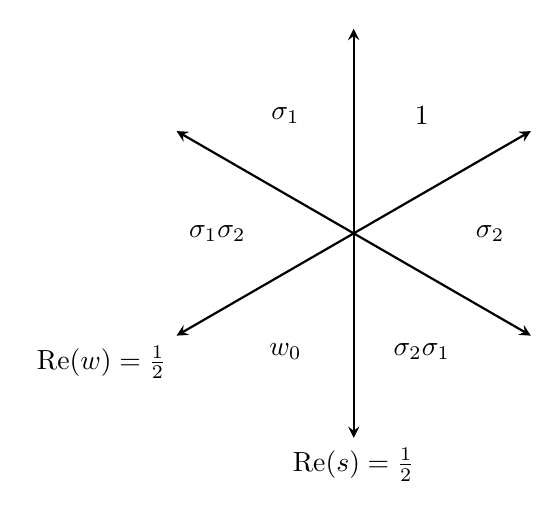
\begin{tikzpicture}[scale=3]
            \draw[thick,-stealth] (0:0) to (30:{sqrt(3)/2});
            \draw[thick,-stealth] (0:0) to (30:{-sqrt(3)/2}) node [below left] {$\Re(w) = \frac{1}{2}$};
            \draw[thick,-stealth] (0:0) to (90:{sqrt(3)/2});
            \draw[thick,-stealth] (0:0) to (90:{-sqrt(3)/2}) node [below] {$\Re(s) = \frac{1}{2}$};
            \draw[thick,-stealth] (0:0) to (150:{sqrt(3)/2});
            \draw[thick,-stealth] (0:0) to (150:{-sqrt(3)/2});

            \node at (60:{sqrt(3)/3}) {$1$};
            \node at (120:{sqrt(3)/3}) {$\s_{1}$};
            \node at (180:{sqrt(3)/3}) {$\s_{1}\s_{2}$};
            \node at (240:{sqrt(3)/3}) {$w_{0}$};
            \node at (300:{sqrt(3)/3}) {$\s_{2}\s_{1}$};
            \node at (0:{sqrt(3)/3}) {$\s_{2}$};
        \end{tikzpicture}
    \end{center}

    In this diagram we have transformed the $(s,w)$-plane so that the origin lies at $\left(\frac{1}{2},\frac{1}{2}\right)$ and the $(s,w)$-axes intersect at $\frac{\pi}{3}$ angles. We have done this so that $\s_{1}$ and $\s_{2}$ act by rigid motions sending the region enclosing $1$ (corresponding to the identity) to either of the adjacent triangles. The other regions are obtained by acting by the corresponding element of $W$. The initial region $\L$ that $Z(s,w)$ is defined on is displayed in the figure below:
    
    \begin{center}
        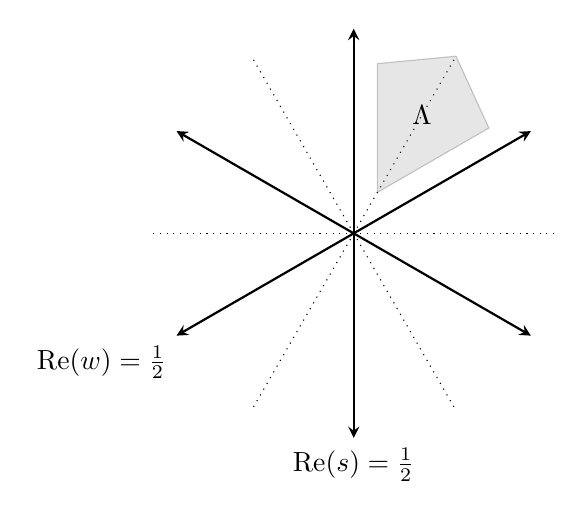
\begin{tikzpicture}[scale=3]
            \draw[dotted](0,0) to (60:{sqrt(3)/2});
            \draw[dotted](0,0) to (240:{sqrt(3)/2});
            \draw[dotted](0,0) to (180:{sqrt(3)/2});
            \draw[dotted](0,0) to (360:{sqrt(3)/2});
            \draw[dotted] (0:0) to (120:{sqrt(3)/2});
            \draw[dotted] (0:0) to (300:{sqrt(3)/2});

            \draw[thick,-stealth] (0:0) to (30:{sqrt(3)/2});
            \draw[thick,-stealth] (0:0) to (30:{-sqrt(3)/2}) node [below left] {$\Re(w) = \frac{1}{2}$};
            \draw[thick,-stealth] (0:0) to (90:{sqrt(3)/2});
            \draw[thick,-stealth] (0:0) to (90:{-sqrt(3)/2}) node [below] {$\Re(s) = \frac{1}{2}$};
            \draw[thick,-stealth] (0:0) to (150:{sqrt(3)/2});
            \draw[thick,-stealth] (0:0) to (150:{-sqrt(3)/2});


            \draw[fill=gray,opacity=0.2] (60:0.2) --+ (0,{((sqrt(5)/3)-0.2)}) -- (60:{sqrt(3)/2}) -- ($(60:0.2)+(30:{((sqrt(5)/3)-0.2)})$) -- cycle;

            \node at (60:{sqrt(3)/3}) {$\L$};
        \end{tikzpicture}
    \end{center}
    
     To meromorphically continue $Z(s,w)$ to all of the $(s,w)$-plane, we first need to show that the quadratic double Dirichlet series $Z_{a_{1},a_{2}}(s,w)$ are locally absolutely uniformly convergent on a slightly larger region than $\L$. This will be achieved by the Phragm\'en-Lindel\"of convexity principal. Fix some small $\e > 0$. The functional equations for $L^{\ast}(s,\chi_{a_{1}d})$ and $L^{\ast}(w,\wtilde{\chi}_{a_{2}m})$ and Stirling's formula together imply the estimates
    \[
        L(-\e,\chi_{a_{1}d}) \ll (a_{1}d)^{\frac{1}{2}+\e} \quad \text{and} \quad L(-\e,\wtilde{\chi}_{a_{2}m}) \ll (a_{2}m)^{\frac{1}{2}+\e},
    \]
    because $L(1+\e,\chi_{a_{1}d}) \ll 1$ and $L(1+\e,\wtilde{\chi}_{a_{2}m}) \ll 1$. As both of these $L$-functions have at most a simple pole at $s = 1$ and $w = 1$ respectively, the Phragm\'en-Lindel\"of convexity principal gives the weak estimates
    \[
        (s-1)L(s,\chi_{a_{1}d}) \ll (a_{1}d)^{\frac{1}{2}+\e} \quad \text{and} \quad (w-1)L(w,\wtilde{\chi}_{a_{2}m}) \ll (a_{2}m)^{\frac{1}{2}+\e},
    \]
    and hence
    \[
        (s-1)L^{(2)}(s,\chi_{a_{1}d}) \ll (a_{1}d)^{\frac{1}{2}+\e} \quad \text{and} \quad (w-1)L^{(2)}(w,\wtilde{\chi}_{a_{2}m}) \ll (a_{2}m)^{\frac{1}{2}+\e},
    \]
    for $\Re(s) > -\e$ and $\Re(w) > -\e$. It follows from the interchange that $(s-1)(w-1)Z_{a_{1},a_{2}}(s,w)$ is locally absolutely uniformly convergent on the region
    \[
        \L_{0} = \L \cup \left\{(s,w) \in \C^{2}:\Re(s) > 0, \Re(w) > \frac{3}{2}\right\} \cup \left\{(s,w) \in \C^{2}:\Re(s) > \frac{3}{2}, \Re(w) > 0\right\}.
    \]
    
    \begin{center}
        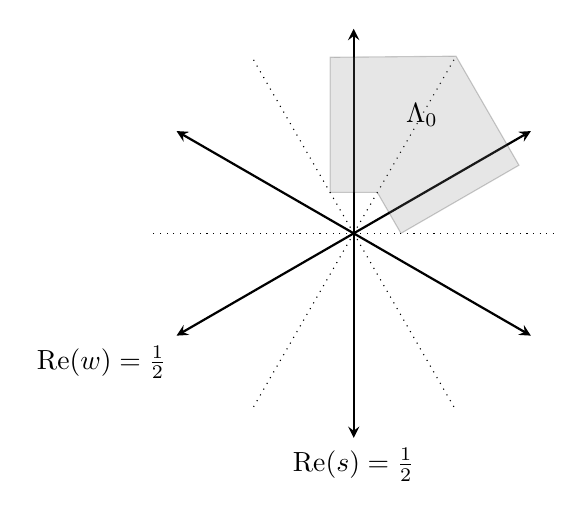
\begin{tikzpicture}[scale=3]
            \draw[dotted](0,0) to (60:{sqrt(3)/2});
            \draw[dotted](0,0) to (240:{sqrt(3)/2});
            \draw[dotted](0,0) to (180:{sqrt(3)/2});
            \draw[dotted](0,0) to (360:{sqrt(3)/2});
            \draw[dotted] (0:0) to (120:{sqrt(3)/2});
            \draw[dotted] (0:0) to (300:{sqrt(3)/2});

            \draw[thick,-stealth] (0:0) to (30:{sqrt(3)/2});
            \draw[thick,-stealth] (0:0) to (30:{-sqrt(3)/2}) node [below left] {$\Re(w) = \frac{1}{2}$};
            \draw[thick,-stealth] (0:0) to (90:{sqrt(3)/2});
            \draw[thick,-stealth] (0:0) to (90:{-sqrt(3)/2}) node [below] {$\Re(s) = \frac{1}{2}$};
            \draw[thick,-stealth] (0:0) to (150:{sqrt(3)/2});
            \draw[thick,-stealth] (0:0) to (150:{-sqrt(3)/2});

            \draw[fill=gray,opacity=0.2] (0:0.2) --+ (30:{cos(30)*((sqrt(3)/2)-0.2)}) -- (60:{sqrt(3)/2}) -- ($(120:0.2)+(0,{sqrt(5)/3-sin(120)*0.2})$) -- (120:0.2) -- (60:0.2) -- cycle;

            \node at (60:{sqrt(3)/3}) {$\L_{0}$};
        \end{tikzpicture}
    \end{center}
    
    Therefore $Z_{a_{1},a_{2}}(s,w)$ is meromorphic on this region with at most polar lines at $s = 1$ and $w = 1$. The key difference between $\L$ and $\L_{0}$ is that $\L_{0}$ intersects the hyperplanes $s = \frac{1}{2}$ and $w = \frac{1}{2}$ so that the union of the reflections $w\L_{0}$ for $w \in W$ is connected. This guarantees that the functional equations imply meromorphic continuation since adjacent reflections of $\L_{0}$ overlap on open sets. We now reflect $\L_{0}$ via the functional equations and then apply a theorem of Bochner which we now state. First, we say that a domain $\W \subset \C^{n}$ is a \textbf{tube domain} if there is an open set $\w \subset \R^{n}$ such that
    \[
        \W = \{(s_{1},\ldots,s_{n}) \in \C^{n}:\Re((s_{1},\ldots,s_{n})) \in \w\}.
    \]
    Tube domains are generalizations of vertical strips in the complex plane. Now we can state the theorem of Bochner (see \cite{hormander2000introduction} for a proof):

    \begin{theorem}[Bochner's continuation theorem]
        If $\W$ is a connected tube domain, then any holomorphic function on $\W$ can be extended to a holomorphic functon on the convex hull $\what{\W}$.
    \end{theorem}

    Clearing polar divisors if necessary, Bochner's continuation theorem implies that any meromorphic function on a connected tube domain posessing a finite amount of hyperplane polar divisors can be extended to a meromorphic function on the convex hull. This is exactly the situation for $Z(s,w)$. Clearly $\L_{0}$ is a tube domain and on $\L_{0}$ there are a most polar lines at $s = 1$ and $w = 1$. Reflecting these hyperplanes via $W$ we obtain the finite set of possible polar divisors:
    \[
        \left\{s = 1, w = 1, s = 0, w = 0, s+w = \frac{1}{2}, s+w = \frac{3}{2}\right\}.
    \]
    So by the previous argument, we are reduced to extending $Z(s,w)$ meromorphically. By applying the functional equations corresponding to $\s_{1}$, $\s_{2}$, and $\s_{1}\s_{2}$, $Z(s,w)$ admits meromorphic continuation to the region
    \[
        \L_{12} = \L_{0} \cup \s_{1}\L_{0} \cup \s_{2}\L_{0} \cup \s_{1}\s_{2}\L_{0}.
    \]

    \begin{center}
        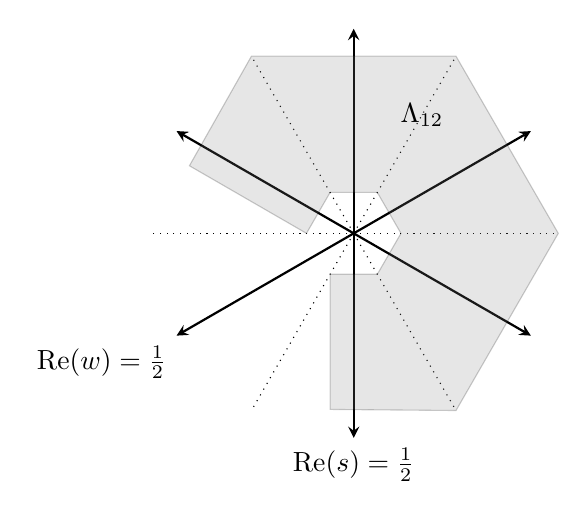
\begin{tikzpicture}[scale=3]
            \draw[dotted](0,0) to (60:{sqrt(3)/2});
            \draw[dotted](0,0) to (240:{sqrt(3)/2});
            \draw[dotted](0,0) to (180:{sqrt(3)/2});
            \draw[dotted](0,0) to (360:{sqrt(3)/2});
            \draw[dotted] (0:0) to (120:{sqrt(3)/2});
            \draw[dotted] (0:0) to (300:{sqrt(3)/2});

            \draw[thick,-stealth] (0:0) to (30:{sqrt(3)/2});
            \draw[thick,-stealth] (0:0) to (30:{-sqrt(3)/2}) node [below left] {$\Re(w) = \frac{1}{2}$};
            \draw[thick,-stealth] (0:0) to (90:{sqrt(3)/2});
            \draw[thick,-stealth] (0:0) to (90:{-sqrt(3)/2}) node [below] {$\Re(s) = \frac{1}{2}$};
            \draw[thick,-stealth] (0:0) to (150:{sqrt(3)/2});
            \draw[thick,-stealth] (0:0) to (150:{-sqrt(3)/2});

            \draw[fill=gray,opacity=0.2] (240:0.2) --+ (0,{-((sqrt(5)/3)+sin(240)*0.2)}) -- (300:{sqrt(3)/2}) -- (0:{sqrt(3)/2}) -- (60:{sqrt(3)/2}) -- (120:{sqrt(3)/2}) -- ($(180:0.2)+(150:{((sqrt(5)/3)+cos(150)*0.2)})$) -- (180:0.2) -- (120:0.2) -- (60:0.2) -- (0:0.2)-- (300:0.2) -- cycle;

            \node at (60:{sqrt(3)/3}) {$\L_{12}$};
        \end{tikzpicture}
    \end{center}

    Now $\L_{12}$ is a connected tube domain whose convex hull is $\C^{2}$. So by applying Bochner's continuation theorem (or rather our comment for meromorphic functions) we see that $Z(s,w)$ admits meromorphic continuation to the $(s,w)$-plane with at most a finite set of polar divisors. This argument is more elegant than repeatedly applying the functional equations corresponding to every $w \in W$. Indeed, if we did we would obtain meromorphic continuation to the region
    \[
        \L_{W} = \bigcup_{w \in W} w\L_{0}.
    \]

    \begin{center}
        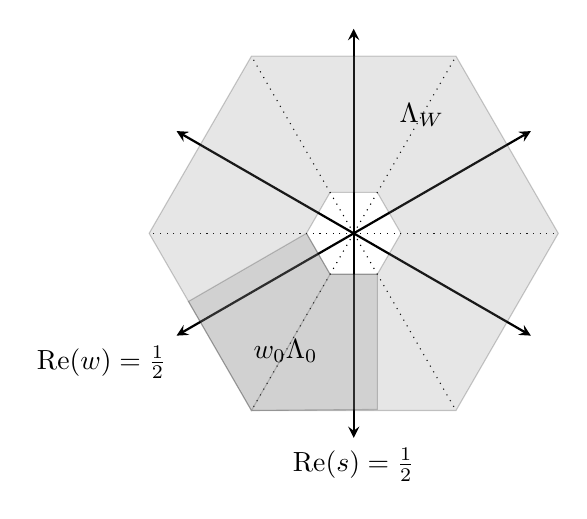
\begin{tikzpicture}[scale=3]
            \draw[dotted](0,0) to (60:{sqrt(3)/2});
            \draw[dotted](0,0) to (240:{sqrt(3)/2});
            \draw[dotted](0,0) to (180:{sqrt(3)/2});
            \draw[dotted](0,0) to (360:{sqrt(3)/2});
            \draw[dotted] (0:0) to (120:{sqrt(3)/2});
            \draw[dotted] (0:0) to (300:{sqrt(3)/2});

            \draw[thick,-stealth] (0:0) to (30:{sqrt(3)/2});
            \draw[thick,-stealth] (0:0) to (30:{-sqrt(3)/2}) node [below left] {$\Re(w) = \frac{1}{2}$};
            \draw[thick,-stealth] (0:0) to (90:{sqrt(3)/2});
            \draw[thick,-stealth] (0:0) to (90:{-sqrt(3)/2}) node [below] {$\Re(s) = \frac{1}{2}$};
            \draw[thick,-stealth] (0:0) to (150:{sqrt(3)/2});
            \draw[thick,-stealth] (0:0) to (150:{-sqrt(3)/2});
        
            \draw[fill=gray,opacity=0.2] (240:{sqrt(3)/2}) -- (300:{sqrt(3)/2}) -- (0:{sqrt(3)/2}) -- (60:{sqrt(3)/2}) -- (120:{sqrt(3)/2}) -- (180:{sqrt(3)/2}) -- (240:{sqrt(3)/2}) -- (240:0.2) -- (180:0.2) -- (120:0.2) -- (60:0.2) -- (0:0.2) -- (300:0.2) -- (240:0.2) -- cycle;

            \draw[fill=gray,opacity=0.2] (180:0.2) --+ (210:{-cos(210)*((sqrt(3)/2)-0.2)}) -- (240:{sqrt(3)/2}) -- ($(300:0.2)+(0,{-((sqrt(5)/3)+sin(300)*0.2)})$) -- (300:0.2) -- (240:0.2) -- cycle; 

            \node at (60:{sqrt(3)/3}) {$\L_{W}$};
            \node at (240:{sqrt(3)/3}) {$w_{0}\L_{0}$};
        \end{tikzpicture}
    \end{center}
    
    There are two issues here. The first is that $Z(s,w)$ has two meromorphic continuations to the region $w_{0}\L_{0}$ given by the functional equations corresponding to $w_{0} = \s_{1}\s_{2}\s_{1}$ and $w_{0} = \s_{2}\s_{1}\s_{2}$ and we would need to show that these agree. The second is that we have not obtained meromorphic continuation to $\C^{2}-\L_{W}$ which is a compact hexagon about the origin. By using Bochner's theorem after meromorphically continuning to $\L_{12}$, we have avoided these issues and as a consquence shown that the meromorphic continuations given by $w_{0} = \s_{1}\s_{2}\s_{1}$ and $w_{0} = \s_{2}\s_{1}\s_{2}$ agree.
\section{Poles \& Residues}
    We can now determine the poles and residues of $Z(s,w)$. Recall that the set of possible polar divisors is
    \[
        \left\{s = 1, w = 1, s = 0, w = 0, s+w = \frac{1}{2}, s+w = \frac{3}{2}\right\}.
    \]
    The poles of $Z(s,w)$ is actually smaller than this set as there are no poles on the hyperplanes $s = 0$, $w = 0$, and $s+w = \frac{3}{2}$. To see this, first observe that by our earlier application of the Phragm\'en-Lindel\"of convexity principal we actually obtained continuation to an open set containing $\L_{0}$ (because our estimates held for $\Re(s) > -\e$ and $\Re(w) > -\e$). We did not need this slightly larger region for the meromorphic continuation but we do require it to study the poles. Now consider the possible polar divisor $s = 0$. Therefore $(s-1)(w-1)Z_{a_{1},a_{2}}(s,w)$ is holomorphic on an open set containing $\L_{0}$ which contains half of the hyperplane defined by $s = 0$ outside of the hexagon $\C^{2}-\L_{W}$. Since $(s-1)(w-1)$ is holomorphic on this region, $Z_{a_{1},a_{2}}(s,w)$ can not have a polar divisor at $s = 0$ on an open set containing $\L_{0}$. Moreover, an open set containing $\s_{1}\s_{2}\L_{0}$ contains the other half of the hyperplane defined by $s = 0$ outside of the hexagon $\C^{2}-\L_{W}$. Upon applying the functional equation corresponding to $\s_{1}\s_{2}$, \cref{nf:thm:double_Dirichlet_series_functional_equation} implies that the gamma factors in the corresponding functional equation have a simple pole when $s+w = \frac{3}{2}$ (the gamma factors in the functional equation for $\s_{1}$ have a simple pole at $s = 1$ and $s-1 \to s+w-\frac{3}{2}$ under $\s_{2}$). Therefore $Z_{a_{1},a_{2}}(s,w)$ does not have polar divisors at $s = 0$ on an open set containing $\s_{1}\s_{2}\L_{0}$ away from $s+w = \frac{3}{2}$. In particular, $Z(s,w)$ does not have a polar divisor at $s = 0$ on $\L_{W}$ and away from the other polar divisors. By Bochner's continuation theorem (after clearing all of the other possible polar divisors), $Z(s,w)$ does not have a polar divisors at $s = 0$ on all of $\C^{2}$ and away from the other polar divisors. An identical argument holds for the case $w = 0$ using the regions $\L_{0}$ and $\s_{2}\s_{1}\L_{0}$. For the polar divisor $s+w = \frac{1}{2}$, we argue in the same way with the regions $\s_{2}\s_{1}\L_{0}$, $\s_{1}\s_{2}\L_{0}$, and $w_{0}\L_{0}$, but there is one difference. For these regions, the gamma factors in the corresponding functional equations are different. For the first two regions $\s_{2}\s_{1}\L_{0}$ and $\s_{1}\s_{2}\L_{0}$, the gamma factors have a simple pole when $s+w = \frac{3}{2}$. For the third region $w_{0}\L_{0}$, the gamma factors have simple poles at $s = 1$ and $w = 1$ which is seen by using both representations $w_{0} = \s_{1}\s_{2}\s_{1}$ and $w_{0} = \s_{2}\s_{1}\s_{2}$. Nevertheless, there are no poles on the hyperplanes $s = 0$, $w = 0$, and $s+w = \frac{1}{2}$ and away from the other polar divisors. As for the hyperplanes $s = 1$, $w = 1$, and $s+w = \frac{3}{2}$, there are clearly genuine poles for $s = 1$ and $w = 1$ coming from $L(s,\chi_{d_{0}})$ and $L(w,\chi_{m_{0}})$ when $d$ and $m$ are perfect squares (so that $d_{0} = m_{0} = 1$). For $s+w = \frac{3}{2}$, we have a pole coming from the gamma factors corresponding to the functional equations for $\s_{2}\s_{1}$ and $\s_{1}\s_{2}$. We collect all of our work as a theorem:

    \begin{theorem}
        $Z(s,w)$ admits meromorphic continuation to $\C^{2}$ with polar divisors $s = 1$, $w = 1$, and $s+w = \frac{3}{2}$.
    \end{theorem}

    We can also study the residues of $Z(s,w)$ at these poles. Since all of the poles are obtained from each other by applying the functional equations of $Z(s,w)$, we begin by looking at the pole when $w = 1$. To compute the residue we use the representation
    \[
        Z(s,w) = \sum_{\substack{m \ge 1 \\ (m,2) = 1}}\frac{L^{(2)}(w,\wtilde{\chi}_{m_{0}})Q_{m_{0}m_{1}^{2}}(w)}{m^{s}},
    \]
    coming from the interchange. The numerator $L(w,\wtilde{\chi}_{m_{0}})Q_{m_{0}m_{1}^{2}}(w)$ in the summand corresponding to $m$ has a pole at $w = 1$ if and only if $m_{0}$ is a perfect square, that is $m_{0} = 1$, or equivalently $m = m_{1}^{2}$ itself is a perfect square. In this case, $L(w,\wtilde{\chi}_{m_{0}}) = \z(w)$ and
    \[
        \Res_{w = 1}L^{(2)}(w,\chi_{m_{0}})Q_{m_{0}m_{1}^{2}}(w) = \frac{1}{2}Q_{m_{1}^{2}}(1).
    \]
    But from \cref{nf:lem:prime_correction_even,nf:thm:correction_polynomial_Euler_product} we see that $Q_{m_{1}^{2}}(1) = 1$, and hence
    \[
        \Res_{w = 1}Z(s,w) = \frac{1}{2}\sum_{\substack{\text{$m$ perfect square} \\ (m,2) = 1}}\frac{Q_{m_{1}^{2}}(1)}{m^{s}} = \frac{1}{2}\sum_{\substack{m \ge 1 \\ (m,2) = 1}}\frac{1}{m^{2s}} = \frac{1}{2}\z^{(2)}(2s).
    \]
    Notice that this expression has a simple pole at $s = \frac{1}{2}$ which is exactly when the polar lines $w = 1$ and $s+w = \frac{3}{2}$ intersect. The residue of $Z(s,w)$ at $s = 1$ is computed in an analogous way. Indeed, by applying the interchange, the exact same argument holds with the roles of $s$ and $w$ interchanged so that
    \[
        \Res_{s = 1}Z(s,w) = \frac{1}{2}\z^{(2)}(2w).
    \]
    Again, this expression has a simple pole at $w = \frac{1}{2}$ which is when the polar lines $s = 1$ and $s+w = \frac{3}{2}$ intersect. The other residues at the simple poles can be computed by applying the functional equations for $Z(s,w)$ and using the residues at $s = 1$ and $w = 1$. Now consider the point where the polar lines $w = 1$ and $s+w = \frac{3}{2}$ intersect. Setting $s = \frac{1}{2}$, we see that $Z\left(\frac{1}{2},w\right)$ has a pole at $w= 1$ and we would like to study this pole more. To achieve this, the Mittag-Leffler theorem applied to $Z(s,w)$ (in $w$) implies
    \[
        Z(s,w) = \frac{R_{1}(s)}{w-1}+\frac{R_{2}(s)}{s+w-\frac{3}{2}}+V(s,w),
    \]
    in some neighborhood of $\left(\frac{1}{2},1\right)$, where $V(s,w)$ is holomorphic, and we have set
    \[
        R_{1}(s) = \Res_{w = 1}Z(s,w) \quad \text{and} \quad R_{2}(s) = \Res_{w = \frac{3}{2}-s}Z(s,w).
    \]
    From our residue computations above, $R_{1}(s) = \frac{1}{2}\z^{(2)}(2s)$ which implies that it has a simple pole at $s = \frac{1}{2}$. The residue is given by $A = \frac{1}{8}$. On the other hand, $Z\left(\frac{1}{2},w\right)$ is holomorphic for $\Re(w) > 1$. These two facts together imply that $R_{2}(s)$ must have a simple pole at $s = \frac{1}{2}$ which cancels the simple pole coming from $R_{1}(s)$. So by Mittag-Leffler again, we may write
    \[
        R_{1}(s) = \frac{A}{s-\frac{1}{2}}+R_{3}(s) \quad \text{and} \quad R_{2}(s) = -\frac{A}{s-\frac{1}{2}}+R_{4}(s),
    \]
    in a neighborhood of $s = \frac{1}{2}$ and where $R_{3}(s)$ and $R_{4}(s)$ are holomorphic. Then
    \begin{align*}
        Z(s,w) &= \frac{R_{1}(s)}{w-1}+\frac{R_{2}(s)}{s+w-\frac{3}{2}}+V(s,w) \\ 
        &= \frac{A}{(w-1)\left(s-\frac{1}{2}\right)}+\frac{R_{3}(s)}{w-1}-\frac{A}{\left(s+w-\frac{3}{2}\right)\left(s-\frac{1}{2}\right)}+\frac{R_{4}(s)}{s+w-\frac{3}{2}}+V(s,w) \\
        &= \frac{A}{(w-1)\left(s+w-\frac{3}{2}\right)}+\frac{R_{3}(s)}{w-1}+\frac{R_{4}(s)}{s+w-\frac{3}{2}}+V(s,w).
    \end{align*}
    We can now set $s = \frac{1}{2}$ and let $B = R_{3}\left(\frac{1}{2}\right)+R_{4}\left(\frac{1}{2}\right)$ so that
    \[
        Z\left(\frac{1}{2},w\right) = \frac{A}{(w-1)^{2}}+\frac{B}{w-1}+O(1).
    \]
    It follows that $Z\left(\frac{1}{2},w\right)$ has a double pole at $w = 1$. This can be thought of as follows: the polar lines $w = 1$ and $s+w = \frac{3}{2}$ correspond to simple poles of $Z(s,w)$ except in the case when they intersect and the order of the poles combine to give $Z\left(\frac{1}{2},w\right)$ a double pole at $w = 1$. Applying the interchange, the exact same argument holds to show that $Z\left(s,\frac{1}{2}\right)$ has a double pole at $s = 1$. We collect this work as a theorem:

    \begin{theorem}\label{nf:thm:double_poles_at_1/2}
        $Z\left(\frac{1}{2},w\right)$ and $Z\left(s,\frac{1}{2}\right)$ have double poles at $w = 1$ and $s = 1$ respectively. In particular, in neighborhoods of $w = 1$ and $s = 1$ respectively, we have
        \[
            Z\left(\frac{1}{2},w\right) = \frac{A}{(w-1)^{2}}+\frac{B}{w-1}+O(1) \quad \text{and} \quad Z\left(s,\frac{1}{2}\right) = \frac{A}{(s-1)^{2}}+\frac{B}{s-1}+O(1),
        \]
        for some constants $A$ and $B$ with $A = \frac{1}{8}$. 
    \end{theorem}

\chapter{A Root Systems Primer}
  \section{Euclidean Vector Spaces}
    Throughout let $V$ be a finite-dimensional Euclidean vector space. That is, $V$ is a finite-dimension vector space over $\R$ endowed with a positive definite symmetric blinear form $(\cdot,\cdot)$. A \textbf{hyperplane} in $V$ is an subspace of codimension $1$. A \textbf{reflection} in $V$ is a invertible linear transformation that fixes some hyperplane and sends any vector orthogonal to that hyperplane to its negative. Clearly reflections are orthogonal transformations ane hence are isometries. Moreover, $V$ has an induced norm $||\cdot|| = \sqrt{\<\cdot,\cdot\>}$ and this norm induces a natural metric topology on $V$ making $V$ a complete metric space. Any nonzero vector $v \in V$ determines its \textbf{reflecting hyperplane} $H_{v}$ defined by
    \[
        H_{v} = \{w \in V:(v,w) = 0\},
    \]
    which is the hyperplane orthogonal to $v$. We say that a vector $w \in V$ lies on the \textbf{positive side} of $H_{v}$ if $(v,w) > 0$ and on the \textbf{negative side} of $H_{v}$ if $(v,w) < 0$. Moreover, any vector proportional to $v$ determines the same reflecting hyperplane. Accordingly, let
    \[
        \s_{v}(w) = w-2\frac{(v,w)}{(v,v)}v, 
    \]
    be the reflection through the hyperplane $H_{v}$. This is indeed a reflection because if $w \in H_{v}$ then $\s_{v}(w) = w$ and $\s_{v}(v) = -v$. Recall that if $v,w \in V$ are orthogonal vectors, that is $(v,w) = 0$, then $\s_{v}\s_{w} = \s_{w}\s_{v}$. Also, if the angle between $v$ and $w$ is $\t$ then $\s_{v}\s_{w}$ is a rotation through angle $2\t$. Lastly, we define an operator $\<\cdot,\cdot\>:(V-\{\mathbf{0}\}) \x (V-\{\mathbf{0}\}) \to \R$ by
    \[
        \<w,v\> = 2\frac{(v,w)}{(v,v)},
    \]
    Note that $\<\cdot,\cdot\>$ is not an inner product as it need not be symmetric and is linear only in the first argument. However, we have the following simplified formula for the reflection $\s_{v}$:
    \[
        \s_{v}(w) = w-\<w,v\>v.
    \]
\section*{Axiomatic Root Systems}
     A \textbf{root system} $\Phi$ in $E$, whose elements $\a \in \Phi$ are called \textbf{roots}, is a finite set of nonzero vectors that satisfty the following properties:

    \begin{enumerate}[label=(\roman*)]
        \item $\Phi$ is a spanning set for $V$.
        \item For any root $\a \in \Phi$, then the only scalar multiples of $\a$ that belong to $\Phi$ are $\a$ itself and $-\a$.
        \item For every root $\a \in \Phi$, $\Phi$ is closed under the reflection $\s_{\a}$.
        \item If $\a,\b \in \Phi$ are roots, then the projection of $\b$ onto the line through $\a$ is an integer or half-integer multiple of $\a$.
    \end{enumerate}

    The last two properties can be equivalently expressed in more algebraic forms:

    \begin{enumerate}[label=(\roman*)]
        \setcounter{enumi}{2}
        \item For any two roots $\a,\b \in \Phi$, $\Phi$ contains the element
        \[
            \s_{\a}(\b) = \b-2\frac{(\a,\b)}{(\a,\a)}\a = \b-\<\b,\a\>\a.
        \]
        \item If $\a,\b \in \Phi$ are roots, then the number $\<\b,\a\> = 2\frac{(\a,\b)}{(\a,\a)}$ is an integer.
    \end{enumerate}
    
    In particular, property (iv) means that $\<\cdot,\cdot\>$ restricted to $\Phi \x \Phi$ is a map of the form $\<\cdot,\cdot\>:\Phi \x \Phi \to \Z$ and so from property (iii) we see that $\s_{\a}$ just adds an integral multiple of $\a$ to $\b$. Sometimes authors omit property (ii) and (iv). In these cases, if (ii) is satisfied we say that the root system is \textbf{reduced} and if (iv) is satisfied we say that the root system is \textbf{crystallographic}. We define the \textbf{rank} of $\Phi$ to be the dimension of $V$. Throughout we will always assume our root systems are reduced and crystallographic (that is they satisfty (i)-(iv)) unless specified otherwise.

    The two simplest examples of root systems are the rank $2$ root systems of type $A_{1}$ and type $A_{2}$:

    \begin{center}
    \begin{tikzpicture}[scale=1.5]
        \draw[thick,-stealth](0,0) to (60:{sqrt(3)/2}) node [above right] {$\a+\b$};
        \draw[thick,-stealth](0,0) to (240:{sqrt(3)/2});
        \draw[thick,-stealth](0,0) to (180:{sqrt(3)/2});
        \draw[thick,-stealth](0,0) to (360:{sqrt(3)/2}) node [right] {$\a$};
        \draw[thick,-stealth] (0:0) to (120:{sqrt(3)/2}) node [above left] {$\b$};
        \draw[thick,-stealth] (0:0) to (300:{sqrt(3)/2});
        
        \draw[dotted,] (0:0) to (30:{sqrt(3)/2});
        \draw[dotted,] (0:0) to (30:{-sqrt(3)/2});
        \draw[dotted,] (0:0) to (90:{sqrt(3)/2});
        \draw[dotted,] (0:0) to (90:{-sqrt(3)/2});
        \draw[dotted,] (0:0) to (150:{sqrt(3)/2});
        \draw[dotted,] (0:0) to (150:{-sqrt(3)/2});

        \node at (0,-1.5) {$A_{2}$};
        
        \begin{scope}[shift = {(-4,0)}]
            \draw[thick,-stealth](0,0) to (180:{sqrt(3)/2});
            \draw[thick,-stealth](0,0) to (360:{sqrt(3)/2}) node [right] {$\a$};
            
            \draw[dotted,] (0:0) to (90:{sqrt(3)/2});
            \draw[dotted,] (0:0) to (90:{-sqrt(3)/2});

            \node at (0,-1.5) {$A_{1}$};
        \end{scope}
    \end{tikzpicture}
    \end{center}

    For these root systems, note that the dotted lines denote the reflections that the corresponding root system is invariant under. In particular, every dotted line is orthogonal to a pair of roots. The root system of type $A_{2}$ will be our running example in our discussion.

    Although we will not use them, we will describe dual root systems. Let $\Phi$ be a root system. For every $\a \in \Phi$ define the \textbf{dual root} $\a^{\vee}$ by
    \[
        \a^{\vee} = \frac{2\a}{(\a,\a)}.
    \]
    Then $\Phi^{\vee} = \{\a^{\vee}:\a \in \Phi\}$ is called the \textbf{dual} to $\Phi$. Clearly $\Phi^{\vee\vee} = \Phi$. Since the dual roots are just scalar multiples of the roots and
    \[
        \<\b^{\vee},\a^{\vee}\> = \left\<\frac{2\b}{(\b,\b)},\frac{2\a}{(\a,\a)}\right\> = \frac{2}{(\b,\b)}\left\<\b,\frac{2\a}{(\a,\a)}\right\> = \frac{4}{(\b,\b)}\frac{\left(\frac{2\a}{(\a,\a)},\b\right)}{\left(\frac{2\a}{(\a,\a)},\frac{2\a}{(\a,\a)}\right)} = 2\frac{(\b,\a)}{(\b,\b)} = \<\a,\b\>,
    \]
    $\Phi^{\vee}$ is also a root system.
\section{Pairs of Roots}
    It turns out that the angles between roots in a root system are quite restricted in general. This is a consequence of property (iv) which implies that $\<\b,\a\>$ and $\<\a,\b\>$ are integers. Without loss of generality we assume $\b \neq \pm \a$, equivalently $\a$ and $\b$ are non-proportional, and there is no additional harm in supposing $|\a| \le |\b|$. If $\t$ is the angle between $\a$ and $\b$, then
    \begin{align*}
        \<\b,\a\>\<\a,\b\> &= 4\frac{(\a,\b)}{(\a,\a)}\frac{(\b,\a)}{(\b,\b)} \\
        &= 4\frac{(\a,\b)^{2}}{|\a|^{2}|\b|^{2}} \\
        &= 4\cos^{2}(\t) \\
        &= (2\cos(\t))^{2},
    \end{align*}
    where in the third line we have made use of the formula $(\a,\b) = |\a||\b|\cos(\t)$. Since this is a square, we see that $\<\b,\a\>$ and $\<\a,\b\>$ must have the same sign. Moreover, since $(2\cos(\t))^{2}$ must be an integer and $2\cos(\t) \in [-2,2]$, we have $\<\b,\a\>\<\a,\b\> \in \{0,1,2,3,4\}$. As $\b \neq \pm \a$ we know $2\cos(\t) \neq \pm 2$ and so $\<\b,\a\>\<\a,\b\> \neq 4$. Combining these facts we see that the only possible values for $\t$ are those given in \cref{tab:root_angles}.

    \begin{table}[ht]
        \caption{}\label{tab:root_angles}
        \begin{stabular}[1.5]{|c|c|c|c|c|c|}
            \hline
            $\t$ & $\cos(\t)$ & $\<\b,\a\>$ & $\<\a,\b\>$ & $\frac{|\b|^{2}}{|\a|^{2}}$ \\
            \hline
            $\frac{\pi}{2}$ & $0$ & $0$ & $0$ & undetermined \\
            \hline
            $\frac{\pi}{3}$ & $\frac{1}{2}$ & $1$ & $1$ & $1$ \\
            \hline
            $\frac{2\pi}{3}$ & $-\frac{1}{2}$ & $-1$ & $-1$ & $1$ \\
            \hline
            $\frac{\pi}{4}$ & $\frac{\sqrt{2}}{2}$ & $2$ & $1$ & $2$ \\
            \hline
            $\frac{3\pi}{4}$ & $-\frac{\sqrt{2}}{2}$ & $-2$ & $-1$ & $2$ \\
            \hline
            $\frac{\pi}{6}$ & $\frac{\sqrt{3}}{2}$ & $3$ & $1$ & $3$ \\
            \hline
            $\frac{5\pi}{6}$ & $-\frac{\sqrt{3}}{2}$ & $-3$ & $-1$ & $3$ \\
            \hline
        \end{stabular}
    \end{table}

    In computing the table we have used the formulas $\<\b,\a\>\<\a,\b\> = (2\cos(\t))^{2}$, $\<\b,\a\> = 2\cos(\t)\frac{|\b|}{|\a|}$, and the assumption $|\a| \le |\b|$. Note that the condition $|\a| \le |\b|$ is only used in the last column to ensure that $\frac{|\b|^{2}}{|\a|^{2}}$ is an integer. Using this table we can prove a very useful lemma:

    \begin{lemma}\label{lem:sum_or_difference_is_a_root}
        Suppose $\a$ and $\b$ are non-proportional roots. If $(\a,\b) > 0$ then $\a-\b$ is a root. If $(\a,\b) < 0$ then $\a+\b$ is a root.
    \end{lemma}
    \begin{proof}
        If $(\a,\b) > 0$ then the angle between $\a$ and $\b$ is strictly acute so that $\cos(\t) > 0$. From \cref{tab:root_angles}, all of these cases correspond to either $\<\a,\b\> = 1$ or $\<\b,\a\> = 1$. If $\<\a,\b\> = 1$, then $\s_{\b}(\a) = \a-\b$ is a root and we are done. If $\<\b,\a\> = 1$, then $\s_{\a}(\b) = \b-\a$ is a root. But then $\s_{\b-\a}(\b-\a) = \a-\b$ is again a root. The second statement follows by using $-\b$ in place of $\b$.
    \end{proof}

    In particular, \cref{lem:sum_or_difference_is_a_root} states that one of $\a-\b$ or $\a+\b$ must be a root. For any two non-proportional roots $\a$ and $\b$, we define the \textbf{$\a$-root string through $\b$} (or simply \textbf{root string}) $S(\a,\b)$ to be the set of all roots of the form $\b+k\a$ for $k \in \Z$. In other words, $S(\a,\b) = \{\b+k\a:k \in \Z\} \cap \Phi $. We can describe this root string explicitely:

    \begin{proposition}\label{prop:sum_or_difference_is_a_root}
        For any two non-proportional roots $\a$ and $\b$, there exsits $u,v \in \Z_{\ge 0}$ such that
        \[
            S(\a,\b) = \{\b-u\a,\ldots,\b+v\a\},
        \]
        and $u-v = \<\b,\a\>$. 
    \end{proposition}
    \begin{proof}
        Let  $u,v \in \Z_{\ge 0}$ be the largest integers for which $\b+v\a \in \Phi$ and $\b-u\a \in \Phi$. Now suppose, by contradiction, that there exists some $k$ with $-u < k < v$ such that $\b+k\a \notin \Phi$. Then we can find integers $r$ and $q$ with $-u \le r < k < q \le v$ such that $\b+r\a \in \Phi$ and $\b+q\a \in \Phi$ but $\b+(r+1)\a \notin \Phi$ and $\b+(q-1)\a \notin \Phi$. By \cref{lem:sum_or_difference_is_a_root} we must have $(\a,\b+r\a) \ge 0$ and $(\a,\b+q\a) \le 0$. Equivalently,
        \[
            (\a,\b)+r(\a,\a) \ge 0 \quad \text{and} \quad (\a,\b)+q(\a,\a) \le 0.
        \]
        But as $(\a,\a) > 0$ and $r < q$ this is impossible. It follows that the root string $S(\a,\b)$ contains every element of the form $\b+k\a$ for $-u \le k \le v$. For the last statement, recall that $\s_{\a}$ acts by adding an integral multiple of $\a$. Therefore the root string $S(\a,\b)$ is left invariant under $\s_{\a}$. But as $\s_{\a}(\a) = -\a$ and $\s_{\a}$ is linear we see that $\s_{\a}$ reverse the root string. So on the one hand, $\s_{\a}(\b+v\a) = \b-u\a$ because $\s_{\a}$ must interchange the two endpoints of the string. On the other hand, linearity implies $\s_{\a}(\b+v\a) = \b-(\<\b,\a\>+v)\a$. Upon combining these two equations we see that $u-v = \<\b,\a\>$.
    \end{proof}

     Note that the number of roots in the string $S(\a,\b)$ is $u+v+1$ (the extra $1$ is there because we need to count $\b$ which corresponds to $\b+k\a$ with $k = 0$). We can actually determine the largest possible length of a root string from \cref{prop:sum_or_difference_is_a_root}. To do this, let $u$ and $v$ be as in \cref{prop:sum_or_difference_is_a_root} and notice that $S(\a,\b)$ and $S(\a,\b+v\a)$ are identical sets. In particular they have the same length. Applying \cref{prop:sum_or_difference_is_a_root} to $S(\a,\b+v\a)$ we get $u+v = \<\b+v\a,\a\>$. But by \cref{tab:root_angles} we know $\<\b+v\a,\a\>$ is at most $3$ (\cref{tab:root_angles} holds for arbitrary non-proportional roots). It follows that $u+v+1$, the length of the root string, is at most $4$.
\section{Bases and Weyl Chambers}
    A \textbf{base} $\D$ for a root system $\Phi$ is a subset of roots, whose elements are call \textbf{simple roots}, satisfying the following propoerties:

    \begin{enumerate}[label=(\roman*)]
        \item $\D$ is a basis for $V$.
        \item Every root $\b \in \Phi$ can be written as a linear combination of simple roots whose coefficients are either all nonnegative intgers or nonpositive integers.
    \end{enumerate}

    Note that if $r$ is the rank of $\Phi$ then property (i) implies $\D$ contains exactly $r$ simple roots. Also, property (ii) takes the following more algebraic form:

    \begin{enumerate}[label=(\roman*)]
        \setcounter{enumi}{1}
        \item Every root $\b \in \Phi$ can be written in the form
        \[
            \b = \sum_{\a \in \D}k_{\a}\a,
        \]
        where either $k_{\a} \ge 0$ or $k_{\a} \le 0$ for all $\a$.
    \end{enumerate}

    Acutally, the expression for $\b$ as a linear combination of simple roots must be unique since $\D$ is a basis for $V$. More generally, let
    \[
        \L_{\Phi} = \bigop_{\a \in \D}\Z\a.
    \]
    be the $\Z$-linear span of the simple roots. We call $\L_{\Phi}$ the \textbf{root lattice} of $\Phi$ relative to $\D$. Then for any $\b \in \L_{\Phi}$ we define the \textbf{height} $h(\b)$ of $\b$ by the formula
    \[
        h(\b) = \sum_{\a \in \D}k_{\a}.
    \]
    If all of the $k_{\a} \ge 0$ we say that $\b$ is \textbf{positive} and if all of the $k_{\a} \le 0$ we say that $\b$ is \textbf{negative}. We write $\b > 0$ and $\b < 0$ for $\b$ being positive or negative respectively. This actually defines a partial ordering $<$ on $\L_{\Phi}$ and hence on $\Phi$ too. Indeed, we say $\b < \a$ if $\a-\b$ is positive and $\b \le \a$ if $\a-\b$ is a positive or $\a = \b$. Accordingly, the set of positive roots is denoted by $\Phi^{+}$ and the set of negative roots by $\Phi^{-}$. Moreover, by property (ii) for root systems we know that $\Phi^{-} = -\Phi^{+}$.

    Unfortunately, the properties of a base $\D$ does not guarentee existance. We will show that every root system admits a base $\D$ (actually many bases). To do this we first set up some notation. For each $v \in V$, let
    \[
        \Phi^{+}(v) = \{\a \in \Phi:(v,\a) > 0\},
    \]
    be the sets of roots lying on the positive side of $H_{v}$. Now notice that the union of finitely many hyperplanes cannot be all of $V$ because $V/H_{v} \cong \R$. Accordingly, we say that $v \in V$ is \textbf{regular} if $v \in V-\bigcup_{\a \in \Phi}H_{\a}$ and is \textbf{singular} otherwise. Note that if $v$ is regular then $\Phi = \Phi^{+}(v)\cup -\Phi^{+}(v)$. Lastly, call $\a \in \Phi^{+}(v)$ \textbf{decomposable} if $\a = \b_{1}+\b_{2}$ for some $\b_{1},\b_{2} \in \Phi^{+}(v)$ and \textbf{indecomposable} otherwise. Let $\D(v)$ be the set of all indecomposable roots in $\Phi^{+}(v)$. Necessarily, $\D(v)$ is finite. It turns out that $\D(v)$ is a base for $\Phi$:

    \begin{theorem}\label{thm:root_system_base}
        If $v \in V$ is regular then $\D(v)$ is a base of $\Phi$, and every base is obtained in this manner.
    \end{theorem}
    \begin{proof}
        We will break the proof into a series of steps. Throughout let $r$ be the rank of $\Phi$.
        \begin{enumerate}
            \item Each root in $\Phi^{+}(v)$ is a nonnegative $\Z$-linear combination of $\D(v)$. If not, then choose $\a \in \Phi^{+}(v)$ such that $\a$ cannot be written in this manner with $(v,\a) > 0$ minimal. Now $\a$ cannot itself be indecomposable so we must have $\a = \b_{1}+\b_{2}$ for some $\b_{1},\b_{2} \in \Phi^{+}(v)$. But then $(v,\a) = (v,\b_{1})+(v,\b_{2})$ where $(v,\b_{1})$ and $(v,\b_{2})$ are positive. But this contradictions the minimality of $(v,\a)$ and the original assertion follows.
            \item If $\a,\b \in \D(v)$ then $(\a,\b) \le 0$ unless $\a = \b$. Again, we argue by contradiction. So suppose $\a \neq \b$ but that $(\a,\b) > 0$. Then \cref{lem:sum_or_difference_is_a_root} implies $\a-\b$ is a root. As $\b \neq -\a$ (for otherwise $\a-\b = 2\a$ which is not a root), either $\a-\b$ or $\b-\a$ is in $\Phi^{+}(v)$. In the first case, $\a = \b+(\a-\b) \in \Phi^{+}(v)$ and in the second case $\b = \a+(\b-\a) \in \Phi^{+}(v)$. Therefore either $\a$ or $\b$ is decomposable. This contradiction proves the original statement.
            \item The set $\D(v)$ is linearly independent. To see this we argue by contradiction. Suppose that
            \[
                \sum_{\a \in \D}k_{\a}\a = 0,
            \]
            for some $k_{\a} \in \R$ not all zero. Seperating the $\a$ for which $k_{\a} > 0$ from those for which $k_{\a} \le 0$ into two indexing sets $\D_{1}$ and $\D_{2}$, which form a partition of $\D$, we can rewrite our linear combination as
            \[
                \sum_{\a \in \D_{1}}k_{\a}\a = \sum_{\b \in \D_{2}}k_{\b}\b,
            \]
            where $k_{\a} > 0$ and $k_{\b} \ge 0$ for all $\a \in \D_{1}$ and $\b \in \D_{2}$ respectively. Denote this expression by $\e$. Then by step (2) we have
            \[
                (\e,\e) = \left(\sum_{\a \in \D_{1}}k_{\a}\a,\sum_{\b \in \D_{2}}k_{\b}\b\right) = \sum_{\substack{\a \in \D_{1} \\ \b \in \D_{2}}}k_{\a}k_{\b}(\a,\b) \le 0,
            \]
            from which it follows that $\e = 0$. Hence $(v,\e) = 0$. But on the other hand
            \[
                (v,\e) = \left(v,\sum_{\a \in \D_{1}}k_{\a}\a\right) = \sum_{\a \in \D_{1}}k_{\a}(v,\a) > 0,
            \]
            because $(v,\a) > 0$ and $k_{\a} > 0$. This contradiction proves $\D(v)$ is linearly independent.
            \item The set $\D(v)$ is a base. We first show property (ii) of a base is satisfied. Indeed, recall that $\Phi = \Phi^{+}(v) \cup -\Phi^{+}(v)$ because $v$ is regular. This fact combined with step (1) proves property (ii). For property (i) of a base, first observe that property (ii) implies $D(v)$ spans $V$ (because $\Phi$ spans $V$). But then step (3) implies $D(v)$ is a basis verifying property (ii).
            \item Lastly, we prove that every base $\D$ is of the form $\D(v)$ for some regular $v$. To begin, we argue that for any base $\D$ there exists a $v \in V$ such that $(v,\a) > 0$ for all $\a \in \D$. To see this, recall that property (i) of a base implies that the simple roots $\a$ form a basis for $V$. Then the dual vectors $\a^{\ast}$ form a basis for $V^{\ast}$. Now consider the linear functional $T:V \to \R^{r}$ in the dual space $V^{\ast}$ defined by
            \[
                T(w) = \sum_{\a \in \D}(w,\a)\a^{\ast}.
            \]
            Clearly $\ker(T) = \{\mathbf{0}\}$ and by the rank-nullity theorem $T$ is a bijection. Then $v = T^{-1}(\sum_{\a \in \D}\a^{\ast})$ is a vector with $(v,\a) = 1 > 0$ for all $\a \in \D$ as desired. Therefore such $v$ exist. Clearly any such $v$ is regular. Since $(v,\a) > 0$ for all $\a \in \D$, property (ii) of a base implies $\Phi^{+} \subseteq \Phi^{+}(v)$ and $\Phi^{-} \subseteq -\Phi^{+}(v)$. It follows that equality holds in both instances. In particular, $\Phi^{+} = \Phi^{+}(v)$ which implies $\D \subset \D(v)$ because the elements of $\D$ are indecomposable ($\D$ is a basis for $V$ so the only linear combination for a simple root is itself). But both $\D$ and $\D(v)$ have $r$ elements so it follows that $\D = \D(v)$.
        \end{enumerate}
    \end{proof}

    \begin{remark}\label{rem:obtuse_independence}
        The arguemnt in part (3) of the proof of \cref{thm:root_system_base} actually shows that any finite set of vectors lying on one side of a hyperplane of $V$ and forming pairwise obtuse angles must be linearly independent.
    \end{remark}

    As $\Phi$ is finite, the the hyperplanes $H_{\a}$, for $\a \in \Phi$, partition $V$ into finitely many connected components. We call each connected componenet of $V-\bigcup_{\a \in \Phi}H_{\a}$ a \textbf{Weyl chamber}. Note that the Weyl chambers are open sets and each regular $v \in V$ belongs to exaclty one Weyl chamber. We denote the Weyl chamber that $v$ belongs to by $\mc{C}(v)$. Then $\mc{C}(v) = \mc{C}(v')$ means that $v$ and $v'$ lie on the same side of the hyperplane $H_{\a}$ for all $\a \in \Phi$. But then part (5) of the proof of \cref{thm:root_system_base} implies $\D(v) = \D(v')$. This means that the Weyl chambers are in a natural bijection with bases of $\Phi$. Accordingly, given a base $\D$ let $\mc{C}(\D)$ be the Weyl chamber defined by $\mc{C}(\D) = \mc{C}(v)$ for any $v$ such that $\D = \D(v)$. We call $\mc{C}(\D)$ the \textbf{fundamental Weyl chamber} relative to $\D$. Equivalently, by part (5) of the proof of \cref{thm:root_system_base} we have
    \[
        \mc{C}(\D) = \{v \in V:(v,\a) > 0 \text{ for all } \a \in \D\}.
    \]
    Conversely, given a Weyl chamber $\mc{C}$, let $\D(\mc{C})$ be the base defined by $\D(\mc{C}) = \D(v)$ for any $v \in \mc{C}$ (note that $v \in \mc{C}$ is automatically regular since it belongs to a Weyl chamber). The fundamental Weyl chamber, and the Weyl chambers in general, will be a very useful tool later on. 
    
    As an example, for the root system of type $A_{2}$, $\D = \{\a,\b\}$ is a base. Indeed, the complete set of roots is $\{-(\a+\b),-\b,-\a,\a,\b,\a+\b\}$ and as the angle between $\a$ and $\b$ is $\frac{2\pi}{3}$ they form a basis for a $2$-dimensional vector space. The corresponding fundamental Weyl chamber is the shaded region below:

    \begin{center}
    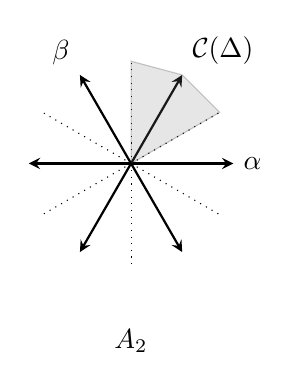
\begin{tikzpicture}[scale=1.5]
        \draw[thick,-stealth](0,0) to (60:{sqrt(3)/2}) node [above right] {$\mc{C}(\D)$};
        \draw[thick,-stealth](0,0) to (240:{sqrt(3)/2});
        \draw[thick,-stealth](0,0) to (180:{sqrt(3)/2});
        \draw[thick,-stealth](0,0) to (360:{sqrt(3)/2}) node [right] {$\a$};
        \draw[thick,-stealth] (0:0) to (120:{sqrt(3)/2}) node [above left] {$\b$};
        \draw[thick,-stealth] (0:0) to (300:{sqrt(3)/2});
        
        \draw[dotted,] (0:0) to (30:{sqrt(3)/2});
        \draw[dotted,] (0:0) to (30:{-sqrt(3)/2});
        \draw[dotted,] (0:0) to (90:{sqrt(3)/2});
        \draw[dotted,] (0:0) to (90:{-sqrt(3)/2});
        \draw[dotted,] (0:0) to (150:{sqrt(3)/2});
        \draw[dotted,] (0:0) to (150:{-sqrt(3)/2});

        \draw[fill=gray,opacity=0.2] (0:0) -- (30:{sqrt(3)/2}) -- (60:{sqrt(3)/2}) -- (90:{sqrt(3)/2}) -- cycle;

        \node at (0,-1.5) {$A_{2}$};
    \end{tikzpicture}
    \end{center}
    
    Given a base $\D$ for $\Phi$, we will require some very useful lemmas about the simple roots $\a \in \D$. Note that the angle between the elements in the base $\D = \{\a,\b\}$ for the type $A_{2}$ root system is obtuse. Our first lemma says that this happens in general:

    \begin{lemma}\label{lem:angles_of_simple_roots_are_obtuse}
        Let $\D$ is a base of $\Phi$ with $\a,\b \in \D$ distinct simple roots. Then $(\a,\b) \le 0$ and $\a-\b$ is not a root.
    \end{lemma}
    \begin{proof}
        Suppose $(\a,\b) > 0$. As $\b \neq -\a$ (for otherwise $\D$ contains $\a$ and $-\a$ and hence is not a basis invalidating property (i) for a base), \cref{lem:sum_or_difference_is_a_root} implies $\a-\b$ is a root. But this contradicts property (ii) for a base. Hence $(\a,\b) \le 0$ and $\a-\b$ is still not a root for otherwise it contradicts property (ii) for a base again.
    \end{proof}

    Our second lemma states that a positive but not simple root is always a sum of a positive root and a simple root:

    \begin{lemma}\label{lem:positive_is_sum_of_simple_base_case}
        If $\a$ is a positive but not simple root, then $\a-\b$ is root for some $\b \in \D$.
    \end{lemma}
    \begin{proof}
        Suppose $(\a,\b) \le 0$ for all $\b \in \D$. Then from \cref{lem:angles_of_simple_roots_are_obtuse} we see that $\D \cup \{\a\}$ form pairwise obtuse angles. By \cref{thm:root_system_base} there exists a $v \in V$ such that $\D = \D(v)$. Then $\D \cup \{\a\}$ all lie on the positive side of $H_{v}$. It follows from \cref{rem:obtuse_independence} that $\D \cup \{\a\}$ is linearly independent which contradictions $\D$ being a basis for $V$ (property (i) for a base). Hence there is some $\b \in \D$ for which $(\a,\b) > 0$. But then \cref{lem:sum_or_difference_is_a_root} implies $\a-\b$ is a root ($\a$ cannot be proportional to $\b$ because $\a$ is not simple).
    \end{proof}

    Note that the root $\a-\b$ in \cref{lem:positive_is_sum_of_simple_base_case} is necessarily positive. Indeed, expressed as a sum of simple roots, $\a-\b$ must have at least one positive coefficient since $\b$ is itself simple and is not proportional to $\a$. By property (ii) of a base it follows that $\a-\b$ is positive. We can actually use \cref{lem:positive_is_sum_of_simple_base_case} to show positive roots can be obtained inductively by adding simple roots:

    \begin{corollary}
        For every $\b \in \Phi^{+}$ there exists, not necessarily distinct, simple roots $\a_{1},\ldots,\a_{k} \in \D$ such that $\b = \a_{1}+\cdots+\a_{k}$ and each partial sum is a root.
    \end{corollary}
    \begin{proof}
        Use \cref{lem:positive_is_sum_of_simple_base_case} and induct on $h(\b)$. 
    \end{proof}
\section{The Weyl Group}
    Throughout this section let $\Phi$ denote a rank $r$. The \textbf{Weyl group} $W$ of $\Phi$ is the subgroup of $\GL(V)$ generated by the reflections $\s_{\a}$ for $\a \in \Phi$. That is,
    \[
        W = \<\s_{\a}:\a \in \Phi\>.
    \]
    If $\D$ is a base for $\Phi$, then the reflection $\s_{\a}$ is said to be a \textbf{simple reflection} if $\a$ is a simple root. Note that property (iii) of a root system implies that $W$ permutes the elements of $\Phi$. Actually, since $\Phi$ is finite this means that $W$ is isomorphic to a subgroup of the symmetric group on $\Phi$. In particular, $W$ is finite. Before proceeding we require a simple lemme about when elements of $\GL(V)$ belong to the Weyl group:

    \begin{lemma}\label{lem:when_linear_transform_is_a_Weyl_group_element}
        Let $\Phi$ be a root system with Weyl group $W$. If $\s \in \GL(V)$ leaves $\Phi$ invariant, fixes pointwise a hyperplane $H$ of $V$, and sends some $\a \in \Phi$ to its negative, then $\s = \s_{\a}$ and $H = H_{\a}$. 
    \end{lemma}
    \begin{proof}
        Let $\tau = \s\s_{\a} = \s\s_{\a}^{-1}$ (the second identity holds because $\s_{\a}$ is a reflection). Then $\tau$ leaves $\Phi$ invariant and $\tau(\a) = \a$. In particular, $\tau$ acts as the identity on the subspace $\R\a$. Actually, the induced action of $\tau$ acts as the identity on the quotient space $V/\R\a$. To see this, since $\s$ fixes $H$ pointwise and sends $\a$ to its negative, we conclude $\a \notin H$. But as $H$ has codimension $1$, it follows that $V = H \op \R\a$. On the other hand, $V = H_{\a} \op \R\a$. These two decompositions together imply $H = H_{\a}$ and so $V/\R\a \cong H_{\a} = H$. It follows that the induced action of $\tau$ on $V/\R\a$ acts as the identity. So all of the eigenvalues of $\tau$ are $1$. But then the minimal polynomial for $\tau$ divides $(T-1)^{r}$. Now choose some $\b \in \Phi$ and let $n > |\Phi|$. Then the roots $\tau(\b),\ldots,\tau^{n}(\b)$ cannot all be distinct so some power of $\tau$ fixes $\b$. Since $|\Phi|$ is finite, choose $n$ large enough so that $\tau^{n}$ fixes $\Phi$ pointwise. Since $\Phi$ spans $V$ (property (i) of a root system), $\tau^{n} = 1$. But then the minimal polynomial for $\tau$ divides $T^{n}-1$. Hence the minimal polynomial divides the $((T-1)^{r},T^{n}-1) = T-1$. But then $\tau = 1$ and using $\tau = \s\s_{\a}^{-1}$ we find that $\s = \s_{\a}$.
    \end{proof}

    We can now show how certain elements of $\GL(V)$ act by conjugation on elements of the Weyl group:

    \begin{lemma}\label{lem:Weyl_group_conjugation}
        Let $\Phi$ be a root system with Weyl group $W$. If $\s \in \GL(V)$ leaves $\Phi$ invariant then $\s\s_{\a}\s^{-1} = \s_{\s(\a)}$ for all $\a \in \Phi$. Moreover, $\<\b,\a\> = \<\s(\b),\s(\a)\>$ for all $\a,\b \in \Phi$.
    \end{lemma}
    \begin{proof}
        Let $\b \in \Phi$ and observe $\s\s_{\a}\s^{-1}(\s(\b)) = \s(\s_{\a}(\b))$. But as $\s_{\a}(\b) \in \Phi$ and by assumption $\s$ leaves $\Phi$ invariant, we conclude $\s(\s_{\a}(\b)) \in \Phi$. Now as $\b$ run over $\Phi$, $\s(\b)$ runs over $\Phi$ and we see that $\s\s_{\a}\s^{-1}$ leves $\Phi$ invariant. Moreover, linearity of $\s$ implies
        \[
            \s\s_{\a}\s^{-1}(\s(\b)) = \s(\s_{\a}(\b)) = \s(\b-\<\b,\a\>\a) = \s(\b)-\<\b,\a\>\s(\a).
        \]
        So taking $\b = \a$ we see that $\s\s_{\a}\s^{-1}(\s(\a)) = -\s(\a)$ because $\<\a,\a\> = 2$. An analgous computation shows $\s\s_{\a}\s^{-1}$ fixes $\s(H_{\a})$ pointwise. So altogether, $\s\s_{\a}\s^{-1}$ leves $\Phi$ invariant, fixes $\s(H_{\a})$ pointwise, and sends $\s(\a) \in \Phi$ to its negative. By \cref{lem:when_linear_transform_is_a_Weyl_group_element}, $\s\s_{\a}\s^{-1} = \s_{\s(\a)}$. But now
        \[
            \s_{\s(\a)}(\s(\b)) = \s(\b)-\<\s(\b),\s(\a)\>\s(\a),
        \]
        and since $\s\s_{\a}\s^{-1} = \s_{\s(\a)}$, we conclude that $\<\b,\a\> = \<\s(\b),\s(\a)\>$.
    \end{proof}

    More generally, we say two root systems $\Phi_{1}$ and $\Phi_{2}$ corresponding to Euclidean vector spaces $V$ are isomorphic if there is an invertible linear transformation $\phi:V \to V$ such that
    \[
        \phi(\Phi_{1}) = \Phi_{2} \quad \text{and} \quad \<\b,\a\> = \<\phi(\b),\phi(\a)\>,
    \]
    for all $\a,\b \in \Phi_{1}$. It follow from \cref{lem:Weyl_group_conjugation} that $\phi$ induces a natural isomorphism on their Weyl groups $W_{1}$ and $W_{2}$ given by $\s \mapsto \phi\s\phi^{-1}$ for $\s \in W_{1}$. More generally, from \cref{lem:Weyl_group_conjugation} we see that an automorphism of $\Phi$ is just an automorphism of $V$ that leaves $\Phi$ invariant. In particular, $W$ is a subgroup of $\Aut(\Phi)$.

    We are now ready for some lemmas about simple reflections. After proving all of these lemmas, we will use them to essentially characterise the Weyl group $W$ with respect to a base $\D$. First up, the simple reflections permute all positive roots except one:

    \begin{lemma}\label{lem:simple_reflections_permute_positive_roots}
        Any simple reflection $\s_{\a}$ permutes the positive roots other than $\a$.
    \end{lemma}
    \begin{proof}
        Let $\b \in \Phi^{+}-\{\a\}$. Recall that $\s_{\a}$ adds a multiple of $\a$ to $\b$ given by
        \[
            \s_{\a}(\b) = \b-\<\b,\a\>\a.
        \]
        As $\b$ is not proportional to $\a$ (the only proportional root is $-\a$ and $\b$ is positive), when $\b$ is expressed as a sum of simple roots it must have a positive coefficient corresponding to some simple root other than $\a$. But then $\s_{\a}(\b)$ must be positive because $\s_{\a}$ only changes the coefficient of $\a$. Moreover, $\s_{\a}(\b) \neq \a$ because $\b \neq -\a$. As $\b$ was an arbitrary positive root and $\s_{\a}$ is a bijection, $\s_{\a}$ must permute the set $\Phi^{+}-\{\a\}$.
    \end{proof}

    As an application of \cref{lem:simple_reflections_permute_positive_roots}, define the \textbf{Weyl vector} $\rho$ to be the half-sum of all the positive roots. In other words, $\rho$ is given by
    \[
        \rho = \frac{1}{2}\sum_{\b > 0}\b.
    \]
    Note that the Weyl vector is not a root because it is not an integral sum of roots. Nevertheless, the action of simple reflections on the Weyl vector is easily expressed:

    \begin{corollary}\label{cor:simple_reflection_on_half_sum_element}
        If $\s_{\a}$ is a simple reflection, then $\s_{\a}(\rho) = \rho-\a$.
    \end{corollary}
    \begin{proof}
        By the linearity of $\s_{\a}$ and \cref{lem:simple_reflections_permute_positive_roots}, we have
        \[
            \s_{\a}(\rho) = \s_{\a}\left(\frac{1}{2}\sum_{\b > 0}\b\right) = \frac{1}{2}\sum_{\substack{\b > 0 \\ \b \neq \a}}\b+\frac{1}{2}\s_{\a}(\a) = \frac{1}{2}\sum_{\substack{\b > 0 \\ \b \neq \a}}\b-\frac{1}{2}\a = \rho-\a.
        \]
    \end{proof}

    Our last lemma tells us when we can remove a simple reflection from a product of simple reflections:

    \begin{lemma}\label{lem:removing_simple_reflection}
        Let $\a_{1},\ldots,\a_{t} \in \D$ be, not necessarily distinct, simple roots. If $\s_{\a_{1}} \cdots \s_{\a_{t-1}}(\a_{t})$ is a negative root, then there exists some $s$ with $1 \le s < t$ such that
        \[
            \s_{\a_{1}} \cdots \s_{\a_{t}} = \s_{\a_{1}} \cdots \s_{\a_{s-1}}\s_{\a_{s+1}} \cdots \s_{\a_{t}}.
        \]
    \end{lemma}
    \begin{proof}
        Set $\b_{i} = \s_{\a_{i+1}} \cdots \s_{\a_{t-1}}(\a_{t})$ for $0 \le i \le t-2$ and $\b_{t-1} = \a_{t}$. Then by assumption $\b_{0} < 0$. But as $\b_{t-1} > 0$, there exists a minimal $s$ with $1 \le s < t$ such that $\b_{s} > 0$. Since $s$ is minimal, $\b_{s-1} = \s_{\a_{s}}(\b_{s}) < 0$. By \cref{lem:simple_reflections_permute_positive_roots}, we find that $\b_{s} = \a_{s}$ and so we know $\s_{\b_{s}} = \s_{\a_{s}}$. But from \cref{lem:Weyl_group_conjugation} we also know
        \[
            \s_{\b_{s}} = (\s_{\a_{s+1}} \cdots \s_{\a_{t-1}})\s_{\a_{t}}(\s_{\a_{s+1}} \cdots \s_{\a_{t-1}})^{-1} = (\s_{\a_{s+1}} \cdots \s_{\a_{t-1}})\s_{\a_{t}}(\s_{\a_{t-1}} \cdots \s_{\a_{s+1}}).
        \]
        Combining these two expressions for $\s_{\b_{s}}$ yields
        \[
            \s_{\a_{s}} = (\s_{\a_{s+1}} \cdots \s_{\a_{t-1}})\s_{\a_{t}}(\s_{\a_{t-1}} \cdots \s_{\a_{s+1}}),
        \]
        and so
        \[
            \s_{\a_{1}} \cdots \s_{\a_{t}} = \s_{\a_{1}} \cdots \s_{\a_{s-1}}\s_{\a_{s+1}} \cdots \s_{\a_{t}}.
        \]
    \end{proof}

    We also have the nice corollary that tells us when we do not have a minimal expression for an element of $W$ in terms of simple reflections:

    \begin{corollary}\label{cor:reflection_of_first_root_is_negative}
        Let $\s \in W$ be a non-identity element and let $\a_{1},\ldots,\a_{t} \in \D$ be, not necessarily distinct, simple roots chosen such that $\s = \s_{\a_{1}} \cdots \s_{\a_{t}}$ with $t$ minimal. Then $\s(\a_{t}) < 0$. 
    \end{corollary}
    \begin{proof}
        Note that as $\s$ is not the identity, $t \ge 1$. If $t = 1$ then $\s = \s_{\a_{t}}$ and the result is trivial. So suppose $t > 2$. Observe, by linearity, that
        \[
            \s(\a_{t}) = \s_{\a_{1}} \cdots \s_{\a_{t-1}}(-\a) = -\s_{\a_{1}} \cdots \s_{\a_{t-1}}(\a).
        \]
        So if $\s(\a_{t}) > 0$ then $\s_{\a_{1}} \cdots \s_{\a_{t-1}}(\a) < 0$ and \cref{lem:removing_simple_reflection} implies that one of the simple reflections $\s_{\a_{s}}$ with $1 \le s < t$ in the expression for $\s$ can be removed. But this contradicts the minimality of $t$. Hence $\s(\a_{t}) < 0$.
    \end{proof}

    Using all of these lemmas we will prove that $W$ permutes the bases of $\Phi$ (equivalently the Weyl chambers) simply transitively and that $W$ is generated by the simple reflections:

    \begin{theorem}\label{thm:Weyl_action_simply_transitively}
        Let $\Phi$ be a root system with base $\D$ and Weyl group $W$. Then the following are true:
        \begin{enumerate}[label=(\roman*)]
            \item If $v \in V$ is regular, then there exists $\s \in W$ such that $(\s(v),\a) > 0$ for all $a \in \D$. In particular, for any chamber $\mc{C}$ there is a $\s \in W$ such that $\s(\mc{C}) = \mc{C}(\D)$.
            \item If $\D'$ is another base of $\Phi$, then $\s(\D') = \D$ for some $\s \in W$.
            \item If $\a$ is any root, then there exists $\s \in W$ such that $\s(\a) \in \D$.
            \item $W$ is generated by the simple reflections $\s_{\a}$ with $\a \in \D$.
            \item If $\s(\D) = \D$ for some $\s \in W$, then $\s = 1$.
            \item If $\s(\mc{C}) = \mc{C}$ for some $\s \in W$, then $\s = 1$.
        \end{enumerate}
    \end{theorem}
    \begin{proof}
        We will prove each statment individually. Let $W'$ be the subgroup of $W$ generated by the simple reflections $\s_{\a}$ with $\a \in \D$. We will first prove statements (i)-(iii) with $W'$ in place of $W$. Call these statements (i')-(iii'). Then we will prove statement (iv), that is $W' = W$, which will imply (i)-(iii). Lastly we will prove statements (v) and (vi).
        \begin{enumerate}[label=(\roman*')]
            \item Choose $\s \in W'$ such that $(\s(v),\rho)$ is as large as possible (such a $\s$ exists because $W'$ is finite). If $\a$ is a simple root, then $\s_{\a}\s \in W'$ and so \cref{cor:simple_reflection_on_half_sum_element} together with the fact that $\s_{\a}$ is an isometry imply
            \[
                (\s(v),\rho) \ge (\s_{\a}\s(v),\rho) = (\s(v)\s_{\a}(\rho)) = (\s(v),\rho-\a) = (\s(v),\rho)-(\s(v),\a).
            \]
            It follows that $(\s(v),\a) \ge 0$ for all $\a \in \D$. By \cref{lem:Weyl_group_conjugation} again, $(\s(v),\a) = (v,\s^{-1}(\a))$. Since $v$ is regular, $(\s(v),\a) = (v,\s(\a)) \neq 0$ for otherwise $v$ is orthogonal to $\s^{-1}(\a) \in \Phi$ which means $v \in H_{\s^{-1}(\a)}$. Therefore we actually have the strict inequality $(\s(v),\a) > 0$ for all $\a \in \D$. The second statement follows immeditely since $v$ was arbitrary.
            \item Since any $\s \in W'$ is a linear isomorphism, it sends a basis to a basis. Therefore $\s(\D')$ satsifies property (i) for a base. Actually, since $\s$ is linear property (ii) for a base is also satisfied. Hence $\s(\D')$ is some base. As $W$ acts by isometries, we have
            \begin{align*}
                \s(\mc{C}(\D')) &= \{\s(v) \in V:(v,\a) > 0 \text{ for all } \a \in \D'\} \\
                &= \{\s(v) \in V:(\s(v),\s(\a)) > 0 \text{ for all } \a \in \D'\} \\
                &= \{v \in V:(v,\s(\a)) > 0 \text{ for all } \a \in \D'\} \\
                &= \{v \in V:(v,\a) > 0 \text{ for all } \a \in \s(\D')\} \\
                &= \mc{C}(\s(\D')),
            \end{align*}
            where the last line follows because $\s(\D')$ is a base. On the other hand, let $v \in \mc{C}(\D')$ so that $\mc{C}(\D') = \mc{C}(v)$. Then by statement (i'), there exists $\s \in W'$ such that $\s(\mc{C}(\D')) = \s(\mc{C}(v)) = \mc{C}(\D)$. Equating these two expressions for $\s(\mc{C}(\D'))$ we find that $\mc{C}(\s(\D')) = \mc{C}(\D)$. Since the Weyl chambers are in bijection with bases, this implies $\s(\D') = \D$.
            \item In light of statement (ii'), it suffices to show that every root $\a \in \Phi$ belongs to some base. To see this, note that the hyperplanes $H_{\b}$ with $\b \neq \pm\a$ are distinct from $H_{\a}$ (because the only root proportional to $\a$ is itself and $-\a$). Since there are finitely many such hyperplanes, we can choose some $v \in H_{\a}$ such that $v \notin H_{\b}$ for all $\b$. Now let $\e > 0$. Then by taking $v' \in V$ close enough to $v$ we guarantee $(v',\a) = \e > 0$ and $|(v',\b)| > \e$ for all $\b$. But then $\a \in \D(v')$.
        \end{enumerate}
       Having verified statements (i')-(iii'), we now prove statement (iv):
        \begin{enumerate}[label=(\roman*)]
            \setcounter{enumi}{3}
            \item It suffices to prove $W' = W$. As $W'$ is a subgroup of $W$, it further suffices to show that $\s_{\a} \in W'$ for every $\a \in \Phi$. By statement (iii'), find $\s \in W'$ such that $\b = \s(\a) \in \D$. But then \cref{lem:Weyl_group_conjugation} implies
            \[
                \s_{\b} = \s_{\s(a)} = \s\s_{\a}\s^{-1}.
            \]
            As $\b$ is a simple root and $\s \in W'$, we conclude $\s_{\a} = \s^{-1}\s_{\b}\s \in W'$.
        \end{enumerate}
        Since we have vertified statement (iv), it follows that (i)-(iii) hold because (i')-(iii') do. At last we prove statements (v) and (vi):
        \begin{enumerate}[label=(\roman*)]
            \setcounter{enumi}{4}
            \item We will prove this by contradiction. suppose $\s(\D) = \D$ but that $\s \neq 1$. By (iv), write $\s$ as a minimal product of simple reflections. But then $\s(\a_{t}) \in \D$ is a positive root which contradicts \cref{cor:reflection_of_first_root_is_negative}. Hence $\s = 1$.
            \item Arguing as in proof of statement (ii'), $\s(\mc{C}) = \mc{C}$ implies $\s(\D(\mc{C})) = \D(\mc{C})$. By (v) it follows that $\s = 1$.
        \end{enumerate}
    \end{proof}

    Note that statements (i) and (vi) of \cref{thm:Weyl_action_simply_transitively} together say that $W$ acts transitively on the Weyl chambers. Similarly, statements (ii) and (v) together say that $W$ acts simply transitively on bases. Since there is a natural bijection between Weyl chambers and bases it follows immeditely that the action of $W$ preserves this correspondence. Also, from statement (iv) we know that every element of $W$ can be written as a product of simple refections for a fixed base $\D$. Accordingly, we define the \textbf{length} $\ell(\s)$ of any non-identity $\s \in W$, relative to $\D$, to be the smallest positive integer such that
    \[
        \s = \s_{\a_{1}} \cdots \s_{\a_{\ell(\s)}},
    \]
    with $\a_{1},\ldots,\a_{\ell(\s)} \in \D$ (not necessarily distinct). We call this expression the \textbf{reduced form} of $\s$ relatively to $\D$. By definition we set $\ell(1) = 0$. We can also characterize the length of roots in another way. For any $\s \in W$ let $n(\s)$ be the number of positive roots $\a \in \Phi^{+}$ such that $\s(\a) \in \Phi^{-}$. Then we have the following proposition:

    \begin{proposition}
        For all $\s \in W$, $\ell(\s) = n(\s)$.
    \end{proposition}
    \begin{proof}
        We will prove this by strong induction on $\ell(\s)$. The case $\ell(\s)$ is clear since then $\s = 1$. Now assume the statement is true for all $\tau \in W$ with $\ell(\tau) < \ell(\s)$. Now suppose $\s = \s_{\a_{1}} \cdots \s_{\a_{\ell(\s)}}$ is the reduced form for $\s$ (where $\a_{1},\ldots,\a_{\ell(\s)} \in \D$). Now for ease of notation set $\a = \a_{\ell(\s)}$. Then \cref{cor:reflection_of_first_root_is_negative} implies $\s(\a) < 0$ and so $\s\s_{\a}(\a) > 0$. But then from \cref{lem:simple_reflections_permute_positive_roots} we see that $n(\s\s_{\a}) = n(\s)-1$. On the other hand, $\ell(\s\s_{\a}) = \ell(\s)-1$. But $\ell(\s)-1 < \ell(\s)$ so by induction our previous two equalities imply $n(\s)-1 = \ell(\s)-1$. Therefore $\ell(\s) = n(\s)$ and the induction is complete.
    \end{proof}

    Returning to the Weyl group, we can also compute the order of the product of two simple reflections:

    \begin{proposition}\label{prop:order_of_product_of_simple_reflections}
        Let $\Phi$ be a root system with base $\D$ and Weyl group $W$. For any two distinct $\a,\b \in \D$, the order of $\s_{\a}\s_{\b}$ is $2$, $3$, $4$, or $6$, depending on if $\<\a,\b\>\<\b,\a\>$ is $0$, $1$, $2$, or $3$ respectively. 
    \end{proposition}
    \begin{proof}
        If $\t$ is the angle between $\a$ and $\b$, then $\s_{\a}\s_{\b}$ is a rotation through angle $2\t$. The statement now follows from \cref{tab:root_angles}.
    \end{proof}

    Lastly, we prove that the closure of the fundamental Weyl chamber $\mc{C}(\D)$ relative to the base $\D$ is a fundamental domain for the action of $W$ on $V$:

    \begin{proposition}\label{prop:fundamental_domain}
        For any base $\D$, $\overline{\mc{C}(\D)}$ is a fundamental domain for the action of $W$ on $V$.
    \end{proposition}
    \begin{proof}
        We first show that every $v \in V$ is $W$-equivalent to some point of $\overline{\mc{C}(\D)}$. This is immediate since $W$ acts simply transitively on the Weyl chambers by \cref{thm:Weyl_action_simply_transitively} and
        \[
            V = \bigcup_{\mc{C}}\overline{\mc{C}}.
        \]
        Now suppose $v,w \in \overline{\mc{C}(\D)}$ and there exists some non-identity $\s \in W$ such that $\s v = w$. We will show $v$ and $w$ lie on the boundary of $\overline{\mc{C}(\D)}$. As the reflections $\s \in W$ are homeomorphisms, they are also open maps. So $v$ and $w$ are either both interior points or both boundary boints. Suppose, to the contrary, that $v,w \in \mc{C}(\D)$. Then as $\s$ is a homeomorphism and $\s(v) = w$, $\s(\mc{C}(\D)) = \mc{C}(\D)$. But then $\s = 1$ because $W$ acts simily transitively on the Weyl chambers. But this contradicts $\s$ being a non-identity element. Hence $v$ and $w$ are on the bounary of $\mc{C}(\D)$. Lastly, $\overline{\mc{C}(\D)}$ is path-connected because $\mc{C}(\D)$ is open and $V$ is complete. Altogether, we have shown that $\mc{C}(\D)$ is a fundamental domain for the action of $W$ on $V$.
    \end{proof}
\section{Irreducible Root Systems}
    It is possible to classify root systems completely. In order to do this, we need the notion of when a root system cannot be decomposed into two smaller root systems. We say that a root system $\Phi$ is \textbf{reducible} if there exists a nontrivial partition $\Phi = \Phi_{1} \cup \Phi_{2}$ such that the roots in $\Phi_{1}$ and $\Phi_{2}$ are pairwise orthogonal. This last condition means $(\Phi_{1},\Phi_{2}) = 0$. Otherwise, we say $\Phi$ is \textbf{irreducible}. Similarly, given a base $\D$ we say that $\D$ is \textbf{reducible} if there exists a nontrivial partition $\D = \D_{1} \cup \D_{2}$ such that the simple roots in $\D_{1}$ and $\D_{2}$ are pairwise orthogonal. Again, this last condition means $(\D_{1},\D_{2}) = 0$. Otherwise, we say $\D$ is \textbf{irreducible}. It turns out that irreducibility of $\Phi$ is equivalent to that of $\D$:
    
    \begin{proposition}\label{prop:irreducibility_equivalence}
        Let $\Phi$ be a root system with base $\D$. Then $\Phi$ is irreducible if and only if $\D$ is.
    \end{proposition}
    \begin{proof}
        We will show the equivalent statement that $\Phi$ is reducible if and only if $\D$ is. So suppose $\Phi = \Phi_{1} \cup \Phi_{2}$ is reducible and note that $(\Phi_{1},\Phi_{2}) = 0$. Unless $\D$ is contained in $\Phi_{1}$ or $\Phi_{2}$, this nontrivial parition of $\Phi$ induces a nontrivial parition $\D = \D_{1} \cup \D_{2}$ with $(\D_{1},\D_{2}) = 0$ as desired. So without loss of generality suppose $\D \subset \Phi_{1}$. Then $(\D,\Phi_{2}) = 0$ and this impies $(V,\Phi_{2}) = 0$ because $\D$ spans $V$. But then $\Phi_{2} = \{\textbf{0}\}$ so that the parition is $\Phi = \Phi_{1} \cup \Phi_{2}$ is trivial which contradicts $\Phi$ being reducible. This proves the ``if'' implication. For the ``only if'', we will prove by contradiction. So suppose $\Phi$ is irreducible but that $\D = \D_{1} \cup \D_{2}$ is reducible. Note that $(\D_{1},\D_{2}) = 0$. By \cref{thm:Weyl_action_simply_transitively} (statement (iii)), every root is the $W$-image of some simple root in $\D$. Therefore the nontrivial decomposition $\D = \D_{1} \cup \D_{2}$ induces a nontrivial decomposition $\Phi = \Phi_{1} \cup \Phi_{2}$ where $\Phi_{i} = W(\D_{i})$ for $1 \le i \le 2$. Now observe that if $(\a,\b) = 0$ then $\s_{\a}(\b) = \b$. Since \cref{thm:Weyl_action_simply_transitively} (statement (iv)) states that $W$ is generated by simple reflections, our previous observation implies that each root in $\Phi_{i}$ is a linear combination of those simple roots in $\D_{i}$ obtained by applying the corresponding $\s \in W$ written as a product of simple reflections. In particular $\Phi_{i}$ is contained in the span of $\D_{i}$. Therefore $(\D_{1},\D_{2}) = 0$ implies $(\Phi_{1},\Phi_{2}) = 0$. But then $\Phi$ is reducible which is a contradiction.
    \end{proof}

    \cref{prop:irreducibility_equivalence} says that to check irreducibility for a root system it suffices to check irreducibility on any base.

    As for some examples, it is clear that the root system of type $A_{2}$ is irreducible. Indeed, no root is orthogonal to all other roots. As for a non-example, the root system of type $A_{1} \x A_{1}$ is the simplest such (here the dotted lines have been supressed because they are covered by roots):

    \begin{center}
    \begin{tikzpicture}[scale=1.5]
        \draw[thick,-stealth](0,0) to (180:{sqrt(3)/2});
        \draw[thick,-stealth](0,0) to (360:{sqrt(3)/2}) node [right] {$\a$};
        \draw[thick,-stealth](0,0) to (90:{sqrt(3)/2}) node [above] {$\b$};
        \draw[thick,-stealth](0,0) to (270:{sqrt(3)/2});

        \node at (0,-1.5) {$A_{1} \x A_{1}$};
    \end{tikzpicture}
    \end{center}
    
    We will now prove some interesting properties of irreducible root systems. The first is that irreducible root systems have a highest root with respect to the partial ordering $<$ induced by height:
    
    \begin{proposition}\label{prop:highest_root}
        Let $\Phi$ be a root system with base $\D$. If $\Phi$ is irreducible then there is a unique maximal root $\b$ relative to the base $\D$ and the partial ordering $<$. Writing $\b = \sum_{\a \in \D}k_{\a}\a$, we have $k_{\a} > 0$ for all $\a$. Moreover, $(\a,\b) \ge 0$ for all $\a \in \D$ and at least one of these inequalities is strict.
    \end{proposition}
    \begin{proof}
        Let $\b = \sum_{\a \in \D}k_{\a}\a$ be maximal with respect to the partial ordering $<$ (such an element exists because $\Phi$ is finite). Clearly $\b > 0$. Now set
        \[
            \D_{1} = \{\a \in \D:k_{\a} > 0\} \quad \text{and} \quad \D_{2} = \{\a \in \D:k_{\a} = 0\}.
        \]
        Then $\D = \D_{1} \cup \D_{2}$ is a partition of $\D$. As $\Phi$ is irreducible, \cref{prop:irreducibility_equivalence} implies that one of $\D_{1}$ or $\D_{2}$ is empty. We will show $\D_{2}$ is empty by contradiction. So suppose $\a \in \D_{2}$. Then $(\a,\b) \le 0$ by \cref{lem:angles_of_simple_roots_are_obtuse}. But $\Phi$ is irreducible so there must be some $\a' \in \D_{1}$ that is not orthogonal to $\a$. By \cref{lem:angles_of_simple_roots_are_obtuse} again, $(\a,\a') < 0$ and therefore $(\a,\b) < 0$. But then \cref{lem:sum_or_difference_is_a_root} implies $\a+\b$ is a root which contradicts the maximality of $\b$. Therefore $\D_{2}$ is empty and thus all $k_{\a} > 0$. Moreover, if $(\a,\b) < 0$ with $\a \in \D$, then arguing just as before, \cref{lem:sum_or_difference_is_a_root} implies $\a+\b$ is a root contradicting the maximality of $\b$. So altogether we have shown $k_{\a} > 0$ and $(\a,\b) \ge 0$ for all $\a \in \D$. In particular, as $\D$ spans $V$ and $\b \neq 0$ there must be some $\a \in \D$ where $(\a,\b) \ge 0$ must be strict. The last thing we have to show is that $\b$ is unique. Suppose $\b'$ is another such maximal root. Then the preceding argument applies to $\b'$ as well and it follows that $(\b,\b') > 0$. By \cref{lem:sum_or_difference_is_a_root}, $\b-\b'$ is a root unless $\b = \b'$. But if $\b-\b'$ is a root then it is either positive or negative so that $\b < \b'$ or $\b' < \b$ both of which contradict the maximality of $\b$ or $\b'$. Hence $\b = \b'$ proving that $\b$ is unique.
    \end{proof}

    We call the unique root $\b$ established in \cref{prop:highest_root} the \textbf{highest root} of $\Phi$ relative to $\D$. Note that as $(\a,\b) \ge 0$ for all $\a \in \D$, $\b \in \overline{C(\D)}$.

    For the type $A_{2}$ root system with base $\D = \{\a,\b\}$, the highest root is $\a+\b$:
    
    \begin{center}
    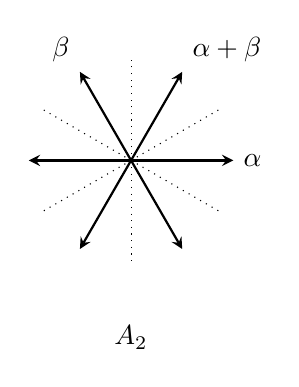
\begin{tikzpicture}[scale=1.5]
        \draw[thick,-stealth](0,0) to (60:{sqrt(3)/2}) node [above right] {$\a+\b$};
        \draw[thick,-stealth](0,0) to (240:{sqrt(3)/2});
        \draw[thick,-stealth](0,0) to (180:{sqrt(3)/2});
        \draw[thick,-stealth](0,0) to (360:{sqrt(3)/2}) node [right] {$\a$};
        \draw[thick,-stealth] (0:0) to (120:{sqrt(3)/2}) node [above left] {$\b$};
        \draw[thick,-stealth] (0:0) to (300:{sqrt(3)/2});
        
        \draw[dotted,] (0:0) to (30:{sqrt(3)/2});
        \draw[dotted,] (0:0) to (30:{-sqrt(3)/2});
        \draw[dotted,] (0:0) to (90:{sqrt(3)/2});
        \draw[dotted,] (0:0) to (90:{-sqrt(3)/2});
        \draw[dotted,] (0:0) to (150:{sqrt(3)/2});
        \draw[dotted,] (0:0) to (150:{-sqrt(3)/2});

        \node at (0,-1.5) {$A_{2}$};
    \end{tikzpicture}
    \end{center}

    The second property is that if the root system $\Phi$ is irreducible, then the Weyl group $W$ acts irreducibly on $V$. That is, there are no nontrivial $W$-invariant subspaces:

    \begin{proposition}\label{prop:Weyl_group_acts_irreducibly}
        If $\Phi$ is irreducible, then $W$ acts irreducibly on $V$.
    \end{proposition}
    \begin{proof}
        Let $U$ be a $W$-invariant supace of $V$. We need to show $U$ is either the zero subspace or all of $V$. Letting $U^{\perp}$ be the orthogonal complement to $U$ in $V$, we have $V = U \op U^{\perp}$. Since $W$ acts by isometries it follows that $U^{\perp}$ is also a $W$-invariant subspace. Now for $\a \in \Phi$, $\s_{\a}$ leaves $H_{\a}$ invariant so either $H_{\a} \subseteq U$ or $H_{\a} \subseteq U^{\perp}$. As $\a$ is orthogonal to $H_{\a}$, in the first case $\a \in U^{\perp}$ and in the second case $\a \in U$. Since $\a$ was an arbitrary root, any root in $\Phi$ either lies in $U$ or $U^{\perp}$. This induces a parition $\Phi = \Phi_{1} \cup \Phi_{2}$ with $\Phi_{1} \subset U$, $\Phi_{2} \subset U^{\perp}$ and $(\Phi_{1},\Phi_{2}) = 0$. Since $\Phi$ is irreducible, this parition must be trivial so that either $\Phi_{1}$ or $\Phi_{2}$ is empty. But as $\Phi_{1}$ spans $U$ and $\Phi_{2}$ spans $U^{\perp}$ (otherwise $\Phi$ does not span $V$ contradicting property (i) of a root system), we must have that either $U$ or $U^{\perp}$ is the zero subspace. Hence $U$ is either the zero subspace or all of $V$.
    \end{proof}

    Our third property is that there are at most two choices for the lengths of the roots in an irreducible root system. Actually, we will show that $W$ acts transitively on the set of roots with the same length:

    \begin{proposition}\label{prop:two_root_lengths}
        If $\Phi$ is irreducible, then there are most two lengths for any root in $\Phi$. Moreover, $W$ acts transitively on the subset of roots with the same length.
    \end{proposition}
    \begin{proof}
        Suppose $\a,\b,\g \in \Phi$ are roots of all different lengths with $|\a| < |\b| < |\g|$. By \cref{prop:Weyl_group_acts_irreducibly} the set $\{\s(\a):\a \in \Phi\}$ spans $V$. Therefore there are elements $\s,\tau \in W$ such that $\a' = \s(\a)$ is not orthogonal to $\b$ and $\a'' = \tau(\a)$ is not orthogonal to $\g$. Moreover, $W$ acts by isometries so that $|\a''| = |\a'| = |\a|$. So from \cref{tab:root_angles}, we see that the ratios $\frac{|\b|^{2}}{|\a|^{2}}$ and $\frac{|\g|^{2}}{|\a|^{2}}$ exist and in particular $\frac{|\b|^{2}}{|\a|^{2}} = 2$ while $\frac{|\g|^{2}}{|\a|^{2}} = 3$. Using \cref{prop:Weyl_group_acts_irreducibly} again but for $\b$, we can find an $\eta \in W$ such that $\beta' = \eta(\beta)$ is not orthogonal to $\g$ and again $|\b'| = |\b|$. But then $\frac{|\g|}{|\b|}$ is defined and from \cref{tab:root_angles} we have $\frac{|\g|^{2}}{|\b|^{2}} \in \left\{2,3\right\}$. On the other hand, our work above implies
        \[
            \frac{|\g|^{2}}{|\b|^{2}} = \frac{|\g|^{2}}{|\a|^{2}}\frac{|\a|^{2}}{|\b|^{2}} = \frac{3}{2},
        \]
        which contradicts \cref{tab:root_angles}. Therefore there are at most two root lengths. We now show that $W$ acts transitively on the subset of roots with the same length. So suppose $\a,\b \in \Phi$ have the same length. Appealing to \cref{prop:Weyl_group_acts_irreducibly} again (replacing $\a$ with $\s(\a)$ for some $\s \in W$ if necessary), we may assume $\a$ and $\b$ are not orthogonal. If $\b = \pm \a$ then the argument is trivial so additionally suppose $\b \neq \pm\a$. As $\frac{|\b|^{2}}{|\a|^{2}} = 1$, we determine from \cref{tab:root_angles} that $\<\b,\a\> = \<\a,\b\> = \pm 1$. Replacing $\b$ by $-\b$ if necessary (we can do this becase $-\b = \s_{\b}(\b)$), we may assume $\<\a,\b\> = 1$. Then
        \[
            \s_{\a}\s_{\b}\s_{\a}(\b) = \s_{\a}\s_{\b}(\b-\a) = \s_{\a}\s_{\b}(\b)-\s_{\a}\s_{\b}(\a) = -\s_{\a}(\b)-\s_{\a}(\a-\b) = -\s_{\a}(\a) = \a.
        \]
        In other words, if $\s = \s_{\a}\s_{\b}\s_{\a}$, then $\s(\b) = \a$. Since $\a$ and $\b$ were arbitrary, it follows that $W$ acts transitively on the subset of roots of the same length.
    \end{proof}

    In accordance with \cref{prop:two_root_lengths}, if an irreducible root system $\Phi$ has two distinct lengths of roots, we call any corresponding root a \textbf{long root} or \textbf{short root} respectively. If every root in an irreducible root system $\Phi$ has the same length, we take the roots to be long by convention. Moreover, in this case we say that $\Phi$ is \textbf{simply laced}.
    
    An example of a non-simply laced root system is that of type $B_{2}$ (here the dotted lines have also been supressed since they are covered by roots):

    \begin{center}
    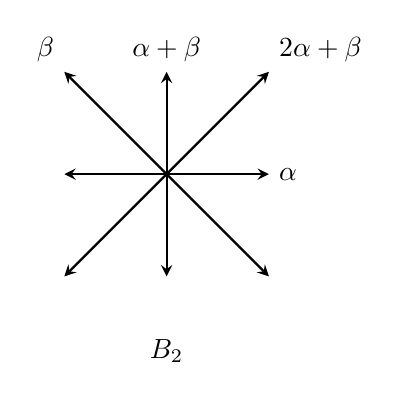
\begin{tikzpicture}[scale=1.5]
        \draw[thick,-stealth](0,0) to (180:{sqrt(3)/2});
        \draw[thick,-stealth](0,0) to (360:{sqrt(3)/2}) node [right] {$\a$};
        \draw[thick,-stealth](0,0) to (90:{sqrt(3)/2}) node [above] {$\a+\b$};
        \draw[thick,-stealth](0,0) to (270:{sqrt(3)/2});
        \draw[thick,-stealth](0,0) to (45:{sqrt(3)/(2*cos(45))}) node [above right] {$2\a+\b$};
        \draw[thick,-stealth](0,0) to (135:{sqrt(3)/(2*cos(45))}) node [above left] {$\b$};
        \draw[thick,-stealth](0,0) to (225:{sqrt(3)/(2*cos(45))});
        \draw[thick,-stealth](0,0) to (315:{sqrt(3)/(2*cos(45))});


        \draw[dotted,] (0:0) to (90:{sqrt(3)/2});
        \draw[dotted,] (0:0) to (90:{-sqrt(3)/2});
        \draw[dotted,] (0:0) to (0:{sqrt(3)/2});
        \draw[dotted,] (0:0) to (0:{-sqrt(3)/2});

        \node at (0,-1.5) {$B_{2}$};
    \end{tikzpicture}
    \end{center}

    For the root system of type $B_{2}$, $\D = \{\a,\b\}$ is a base, $\b$ is the long root while $\a$ is the short root and $2\a+\b$ is the highest root relative to the base $\D$.
    
    If $\D$ is a base of $\Phi$, then the highest root $\b$ established in \cref{prop:highest_root} is always long:

    \begin{proposition}
        Let $\Phi$ be an irreducible root system with base $\D$. Then the highest root $\b$ relative to $\D$ is long.
    \end{proposition}
    \begin{proof}
        This is trivial if $\Phi$ is simply laced so suppose otherwise. It suffices to show that $(\b,\b)\ge (\a,\a)$ for all $\a \in \Phi$. Since $W$ acts by isometries and $\mc{C}(\D)$ is a fundamental domain for $W$ by \cref{prop:fundamental_domain}, we may assume $\a \in \overline{\mc{C}(\D)}$. As $\b-\a > 0$ by \cref{prop:highest_root}, we have $(v,\b-\a) \ge 0$ for any $v \in \overline{\mc{C}(\D)}$. Recalling that $\b \in \overline{\mc{C}(\D)}$ (this is also a consequence of \cref{prop:highest_root}), we may take $v = \b$ and conclude that $(\b,\b-\a) \ge 0$ which is equivalent to $(\b,\b) \ge (\b,\a)$. On the other hand, $\a \in \overline{\mc{C}(\D)}$ and $\b-\a > 0$ together imply $(\b-\a,\a) \ge 0$ which is equivalent to $(\b,\a) \ge (\a,\a)$. Combining our two inequalities involving $(\b,\a)$ gives $(\b,\a) \ge (\a,\a)$ as desired.
    \end{proof}
\section{Dynkin Diagrams \& Classification}
    Irreducible root systems have been completely classified. We will only state the classification in terms of Dynkin diagrams. First, we define the Coxeter diagram of a root system. So let $\Phi$ be a root system of rank $r$ with base $\D$. We will enumerate the base by writing the simple roots as $\a_{i}$ for $1 \le i \le r$. We define the \textbf{Dynkin diagram} of $\Phi$ to be the graph having $r$ vertices represented by the $\a_{i}$ such that $\a_{i}$ is joined to $\a_{j}$ by $\<\a_{i},\a_{j}\>\<\a_{j},\a_{i}\>$ edges. Moreover, in the case $\Phi$ is not simply laced we add arrow pointing from $\a_{i}$ to $\a_{j}$ if $\a_{j}$ is a long root. Note that from \cref{tab:root_angles}, $\<\a_{i},\a_{j}\>\<\a_{j},\a_{i}\> \in \{0,1,2,3\}$. It is not hard to show that the Dynkin diagram of $\Phi$ determines $\Phi$ and is independent of base:

    \begin{proposition}\label{prop:Dynkin_diagram_unique}
        The Dynkin diagram of $\Phi$ determines $\Phi$ and is independent of base. 
    \end{proposition}
    \begin{proof}
        Let $\Phi$ be a root system of rank $r$ with base $\D$ and let $\a_{i}$ for $1 \le i \le r$ be the simple roots. If $\t$ is the angle between $\a_{i}$ and $\a_{j}$ then from the equation $\<\a_{i},\a_{j}\> = 2\cos(\t)\frac{|\a_{i}|}{|\a_{j}|}$, the number of edges and possible arrow between $\a_{i}$ and $\a_{j}$ in the Dynkin diagram determines the exact values of $\<\a_{i},\a_{j}\>$ and $\<\a_{j},\a_{i}\>$ as given in \cref{tab:root_angles}. But then the reflections $\s_{\a_{i}}$ for $1 \le i \le r$ are completely determined and from \cref{thm:root_system_base} and \cref{thm:Weyl_action_simply_transitively} (statement (iv) in particular) this determines the roots in $\Phi$ completely. Now let $\D'$ be another base for $\Phi$ with simple roots $\a_{i}'$ for $1 \le i \le r$. From \cref{thm:Weyl_action_simply_transitively} (statement (ii)) there is a $\s \in W$ such that $\s(\D') = \D$. Relabeling if necessary, we may assume $\s(\a_{i}') = \a_{i}$. But as $W$ acts by isometries, $\<\s(\a_{i}'),\s(\a_{j}')\> = \<\a_{i},\a_{j}\>$ for all $1 \le i \le j \le r$. Moreover, \cref{prop:two_root_lengths} implies that $\s$ preserves root lengths. These two statements together mean that the Dynkin diagrams for $\D$ and $\D'$ are identical.
    \end{proof}

    For the type $A_{2}$ root system, the system itelf and its corresponding Dynkin diagram are displayed below:
    
    \begin{center}
    \begin{tikzpicture}[scale=1.5]
        \draw[thick,-stealth](0,0) to (60:{sqrt(3)/2});
        \draw[thick,-stealth](0,0) to (240:{sqrt(3)/2});
        \draw[thick,-stealth](0,0) to (180:{sqrt(3)/2});
        \draw[thick,-stealth](0,0) to (360:{sqrt(3)/2}) node [right] {$\a_{1}$};
        \draw[thick,-stealth] (0:0) to (120:{sqrt(3)/2}) node [above left] {$\a_{2}$};
        \draw[thick,-stealth] (0:0) to (300:{sqrt(3)/2});
        
        \draw[dotted,] (0:0) to (30:{sqrt(3)/2});
        \draw[dotted,] (0:0) to (30:{-sqrt(3)/2});
        \draw[dotted,] (0:0) to (90:{sqrt(3)/2});
        \draw[dotted,] (0:0) to (90:{-sqrt(3)/2});
        \draw[dotted,] (0:0) to (150:{sqrt(3)/2});
        \draw[dotted,] (0:0) to (150:{-sqrt(3)/2});

        \node at (0,-1.5) {$A_{2}$};
        
        \begin{scope}[shift = {(4,0)}]
            \node at (0,0) { \scalebox{1.5}{\dynkin[labels={\a_{1},\a_{2}},edge length=1cm]A2}};
        \end{scope}
    \end{tikzpicture}
    \end{center}

    \cref{prop:Dynkin_diagram_unique} implies that in order to classify root systems it suffices to determine the possible Dynkin diagrams. It also implies that we don't need to numerate the vertices of the Dynkin diagram by $\a_{i}$ (since the diagram is independent of the choice of base), and we only need to understand that the vertices represent simple roots. Actually, it suffices to determine the Dynkin diagrams only for irreducible root systems. Indeed, from \cref{tab:root_angles} we see that there no edge between simple roots $\a_{i}$ and $\a_{j}$ in the Dynkin diagram if and only if these simple roots are orthogonal. It follows from \cref{prop:irreducibility_equivalence} that $\Phi$ is irreducible if and only if its Dynkin diagram is connected. Moreover, the Dynkin diagram of any reducible root system is a disjoint union of finitely many connected Dynkin diagrams (corresponding to irreducible root systems). The Dynkin diagrams of irreducible root systems have been completely classified (for a proof see \cite{humphreys1972introduction}):
    
    \begin{theorem}\label{thm:Dynkin_diagram_classification}
        If $\Phi$ is a rank $r$ an irreducible root system, its Dynkin diagram is one of the following types:
        \begin{center}
        \begin{stabular}[1]{cc}
            $A_{r} \text{ for } r \ge 1:$ & \scalebox{1.5}{$\dynkin A{}$} \\
            $B_{r} \text{ for } r \ge 2:$ &  \scalebox{1.5}{$\dynkin B{}$} \\
            $C_{r} \text{ for } r \ge 3:$ &  \scalebox{1.5}{$\dynkin C{}$} \\
            $D_{r} \text{ for } r \ge 4:$ &  \scalebox{1.5}{$\dynkin D{}$} \\
            $E_{6}$ &  \scalebox{1.5}{$\dynkin E6$} \\
            $E_{7}$ &  \scalebox{1.5}{$\dynkin E7$} \\
            $E_{8}$ &  \scalebox{1.5}{$\dynkin E8$} \\
            $F_{4}$ &  \scalebox{1.5}{$\dynkin F4$} \\
            $G_{2}$ &  \scalebox{1.5}{$\dynkin G2$} \\
        \end{stabular}
        \end{center}
        where in each diagram it is understood that there are $r$ many vertices.
    \end{theorem}

    It is worth mentioning a couple of remarks about \cref{thm:Dynkin_diagram_classification}. Often when discussing root systems with respect to this classification we supress the rank and only speak of the letter type. Accordingly, Dynkin diagrams, or their associated root systems, of type $A$, $B$, $C$, and $D$ are said to be of \textbf{standard} type. In \cref{thm:Dynkin_diagram_classification}, the conditions placed upon the rank for these types is so that there are no redundancies in the classification. Dynkin diagrams and root systems of types $E$, $F$, and $G$ are said to be of \textbf{exceptional type}. Clearly there are finitely many root systems of exceptional type.

\chapter{Quadratic Weyl Group Multiple Dirichlet Series Over Function Fields}
  \section{Preliminaries}
    \subsection*{Function Fields}
        We present an overview of the zeta function and Dirichlet $L$-functions attached to $\F_{q}(t)$. For a detailed discussion see \cite{rosen2002number}. Let $q$ be a power of an odd prime and let $\F_{q}[t]$ be the polynomial ring in $t$ with coefficients in the finite field $\F_{q}$. This is a principal ideal domain. Moreover, the nonzero prime ideals in $\F_{q}[t]$ are generated by irreducible polynomials. Let $\F_{q}(t)$ denote the quotient field. Define the norm function $N(m)$ by
        \[
            N(m) = |m| = q^{\deg(m)},
        \]
        for any $m \in \F_{q}[t]$. The zeta function $\z(s)$ on $\F_{q}[t]$ is defined as the Dirichlet series or Euler product
        \[
            \z(s) = \sum_{\text{$m$ monic}}\frac{1}{|m|^{s}} = \prod_{\text{$P$ monic irr}}\left(1-\frac{1}{|P|^{s}}\right)^{-1},
        \]
        where the second equality holds since $\F_{q}[t]$ is a unique factorization domain. As for questions of convergence, there are $q^{n}$ monic polynomials of degree $n$ so, provided $\Re(s) > 1$, we can sum up the Dirichlet series according to degree and obtain an explicit expression:
        \[
            \z(s) = \sum_{n \ge 0}\frac{\text{\# of monic poly of deg $n$}}{q^{ns}} = \sum_{n \ge 1}\frac{1}{q^{n(1-s)}} = \frac{1}{1-q^{1-s}}.
        \]
        The latter expression is meromorphic on $\C$ with a simple pole at $s = 1$ of residue $\frac{1}{\log(q)}$. Therefore $\z(s)$ admits meromorphic continuation to $\C$. The zeta function also satisfies a functional equation. Define the completed zeta function (this is also the zeta function attached to $\F_{q}(t)$) by
        \[
            \z^{\ast}(s) = \frac{1}{1-q^{-s}}\z(s).
        \]
        Then
        \[
            \z^{\ast}(s) = q^{2s-1}\z^{\ast}(1-s).
        \]
        Recall that characters on $\F_{q}[t]$ are multiplicative functions $\chi:\F_{q}[t] \to \C$. The two flavors we will care about are:
        
        \begin{itemize}
            \item Dirichlet characters: multiplicative functions $\chi_{d}:\F_{q}[t] \to \C$ modulo $d \in \F_{q}[t]$ (in that they are $d$-periodic) and such that $\chi_{d}(m) = 0$ if $(m,d) > 1$.
            \item Hilbert symbols: Dirichlet characters modulo $1$.
        \end{itemize}
        
        In either case, the image always lands in the roots of unity. If $\chi$ is a Dirichlet character then its conjugate $\conj{\chi}$ is also a Dirichlet character. Moreover, $\conj{\chi}$ is the multiplicative inverse to $\chi$ and the Dirichlet characters modulo $d$ form a group under multiplication. This group is always finite and its order is $\phi(d) = |(\F_{q}[t]/d\F_{q}[t])^{\x}|$. Dirichlet characters also satisfy orthogonality relations:

        \begin{theorem}[Orthogonality relations]
            \phantom{ }
            \begin{enumerate}[label=(\roman*)]
            \item For any two Dirichlet characters $\chi$ and $\psi$ modulo $d$,
            \[
                \frac{1}{\phi(d)}\psum_{f \tmod{d}}\chi(f)\conj{\psi}(f) = \d_{\chi,\psi}.
            \]
            \item For any $f,g \in (\F_{q}[t]/d\F_{q}[t])^{\x}$,
            \[
                \frac{1}{\phi(d)}\sum_{\chi \tmod{d}}\chi(f)\cchi(g) = \d_{f,g}.
            \]
            \end{enumerate}
        \end{theorem}

        The Dirichlet characters that are of interest to us are those given by the quadratic residue symbol on $\F_{q}[t]$. First let us recall this symbol. For any irreducible $p \in \F_{q}[t]$ and any $m \in \F_{q}[t]$, we define the quadratic residue symbol $\tlegendre{m}{p}$ by
        \[
            \legendre{m}{p} \equiv m^{\frac{|p|-1}{2}} \tmod{p} = \begin{cases} 1 & \text{if $x^{2} \equiv m \tmod{p}$ is solvable}, \\ -1 & \text{if $x^{2} \equiv m \tmod{p}$ is not solvable}, \\ 0 & \text{if $m \equiv 0 \tmod{p}$}. \end{cases}
        \]
        This symbol is only dependent upon $m$ modulo $p$ and is multiplicative in $m$. Moreover, if $b \in \F_{q}^{\ast}$, we have
        \[
            \legendre{b}{p} = \sgn(b)^{\deg(p)}.
        \]
        where $\sgn(b) = \pm1$ depending on if $b \in (\F_{q}^{\x})^{2}$ or not. For $m \in \F_{q}[t]$ we define $\sgn(m) = \sgn(b_{n})$ if $m(t) = b_{n}t^{n}+b_{n-1}t^{n+1}+\cdots+b_{0}$ (with $b_{n} \neq 0$). We can extend the quadratic residue symbol multiplicatively in the denomator. If $d = bp_{1}^{e_{1}}p_{2}^{e_{2}} \cdots p_{k}^{e_{k}}$ is the prime factorization of $d$ (with $b \in \F_{q}^{\ast}$), then we define
        \[
            \legendre{m}{d} = \prod_{1 \le i \le k}\legendre{m}{p_{i}}^{e_{i}}.
        \]
        So the quadratic residue symbol now makes sense for any nonzero $d \in \F_{q}[t]$. Morevoer, it only depends upon $m$ modulo $d$, the ideal generated by $d$, and is multiplicative in $d$. The quadratic residue symbol also admits the following reciprocity law:

        \begin{theorem}[Quadratic reciprocity]
            If $d,m \in \F_{q}[t]$ are relatively prime and nonzero, then
            \[
                \legendre{d}{m} = (-1)^{\frac{q-1}{2}\deg(d)\deg(m)}\sgn(d)^{\deg(m)}\sgn(m)^{-\deg(d)}\legendre{m}{d}.
            \]
        \end{theorem}

        Note that if $q \equiv 1 \tmod{4}$ and $d$ and $m$ are monic, then the sign in the statement of quadratic reciprocity is always $1$ so that reciprocity is perfect:
        \[
            \legendre{d}{m} = \legendre{m}{d}.
        \]
        We can now define the quadratic Dirichlet characters. For any nonzero square-free monic $d \in \F_{q}[t]$, define the quadratic Dirichlet character $\chi_{d}$ by the following quadratic residue symbol:
        \[
            \chi_{d}(m) = \legendre{d}{m}.
        \]
        This quadratic Dirichlet character is attached to the quadratic extension $\F_{q}(t)(\sqrt{d})$. If $b \in \F_{q}^{\x}$, we define $\chi_{b}$ by
        \[
            \chi_{b}(m) = \legendre{b}{m} = \sgn(b)^{\deg(m)}.
        \]
        We extend $\chi_{d}$ multiplicatively in the denominator so that $\chi_{d}$ makes sense for any nonzero $d \in \F_{q}[t]$. In particular, $\chi_{d}(m) = \pm1$ provided $d$ and $m$ are relatively prime and $\chi_{d}(m) = 0$ if $(m,d) > 1$. Quadratic reciprocity implies that $\chi_{d}$ is a Dirichlet character modulo $d$. Indeed, for any $m$ we can take $d$ modulo $m$ so that $\deg(d+m) = \deg(m)$ and $\sgn(d+m) = \sgn(m)$. Lastly, note that if $q \equiv 1 \tmod{4}$ and $d$ and $m$ are monic,
        \[
            \chi_{d}(m) = \chi_{m}(d),
        \]
        is a reformulation of reciprocity being perfect. We now discuss the Hilbert symbols. The only ones we will need are those given by the quadratic reisdue symbol. There are only two of them: one nontrivial and one trivial. The nontrivial Hilbert symbol $\psi$ is defined by
        \[
            \psi(m) = (-1)^{\deg(m)}.
        \]
        The other Hilbert symbol is $\psi^{2} = \chi_{1}$. To see that $\psi$ is given by a quadratic Dirichlet character, just notice that for $\t \in \F^{\x}-(\F^{\x})^{2}$ we have $\chi_{\t}(m) = (-1)^{\deg(m)}$. The Hilbert symbols are necessary because they control the possible sign change in the statement of quadratic reciprocity coming from the $\sgn(d)^{\deg(m)}$ and $\sgn(m)^{-\deg(d)}$ factors. Technically speaking, we would also require Hilbert symbols to keep track of the $(-1)^{\frac{q-1}{2}\deg(d)\deg(m)}$ factor but as we will assume $q \equiv 1 \tmod{4}$, we will not discuss this additional difficulty.

        We are now ready to discuss the $L$-functions associated to quadratic Dirichlet characters. We define the $L$-function $L(s,\chi_{d})$ attached to $\chi_{d}$ by a Dirichlet series or Euler product:
        \[
            L(s,\chi_{d}) = \sum_{\text{$m$ monic}}\frac{\chi_{d}(m)}{|m|^{s}} = \prod_{\text{$P$ monic irr}}\left(1-\frac{\chi_{d}(P)}{|P|^{s}}\right)^{-1}.
        \]
        By definition of the quadratic Dirichlet character, $L(s,\chi_{d}) \ll \z(s)$ for $\Re(s) > 1$ so that $L(s,\chi_{d})$ is locally absolutely uniformly convergent in this region. $L(s,\chi_{d})$ also admits meromorphic continuation to $\C$ with a simple pole at $s = 1$ if $d$ is a perfect square and is analytic otherwise (see \cite{rosen2002number} for a proof). The completed $L$-function is defined as follows:
        \[
            L^{\ast}(s,\chi_{d}) = \begin{cases} \frac{1}{1-q^{-s}}L(s,\chi_{d}) & \text{if $\deg(d)$ is even}, \\ L(s,\chi_{d}) & \text{if $\deg(d)$ is odd}, \end{cases}
        \]
        and satisfies the functional equation
        \[
            L^{\ast}(s,\chi_{d}) = \begin{cases} q^{2s-1}|d|^{\frac{1}{2}-s}L^{\ast}(1-s,\chi_{d}) & \text{if $\deg(d)$ is even}, \\ q^{2s-1}(q|d|)^{\frac{1}{2}-s}L^{\ast}(1-s,\chi_{d}) & \text{if $\deg(d)$ is odd}. \end{cases}
        \]
        Note that in the case $\deg(d)$ is even, the conductor is $|d|$ and in the case $\deg(d)$ is odd, the conductor is $q|d|$. In other words, the gamma factors depend upon the degree of $d$.
    \subsection*{Root Systems}
        Throughout let $V$ be an $r$-dimensional Euclidean vector space with standard inner product $(\cdot,\cdot)$. For any nonzero $v \in V$, let
        \[
            H_{v} = \{u \in V:(v,u) = 0\},
        \]
        be the hyperplane perpendicular to $v$. Accordingly, let
        \[
            s_{v}(w) = w-2\frac{(v,w)}{(v,v)}v, 
        \]
        be the reflection through the hyperplane $H_{v}$. Lastly, we will define an operator $\<\cdot,\cdot\>:V \x V \to \R$ by
        \[
            \<w,v\> = 2\frac{(v,w)}{(v,v)},
        \]
        Note that $\<\cdot,\cdot\>$ is not an inner product as it need not be symmetric and is linear only in the first argument. However, we have the simplified formula
        \[
            s_{v}(w) = w-\<w,v\>v.
        \]
        Recall that a root system $\Phi$ in $V$, whose elements $\a \in \Phi$ are called roots, is a finite set of nonzero vectors that satisfty the following conditions:

        \begin{enumerate}[label=(\roman*)]
            \item $\Phi$ is a spanning set for $V$.
            \item For any root $\a \in \Phi$, then the only scalar multiples of $\a$ that belong to $\Phi$ are $\a$ itself and $-\a$.
            \item For every root $\a \in \Phi$, $\Phi$ is closed under the reflection $s_{\a}$ through the hyperplane $H_{\a}$ perpendicular to $\a$.
            \item If $\a,\b \in \Phi$ are roots, then the projection of $\b$ onto the line through $\a$ is an integer or half-integer multiple of $\a$.
        \end{enumerate}

        The last two conditions can be equivalently expressed in more algebraic forms:

        \begin{enumerate}[label=(\roman*)]
            \setcounter{enumi}{2}
            \item For any two roots $\a,\b \in \Phi$, $\Phi$ contains the element
            \[
                s_{\a}(\b) = \b-2\frac{(\a,\b)}{(\a,\a)}\a = \b-\<\b,\a\>\a.
            \]
            \item If $\a,\b \in \Phi$ are roots, then the number $\<\b,\a\> = 2\frac{(\a,\b)}{(\a,\a)}$ is an integer.
        \end{enumerate}
        
        We suppose that our root system $\Phi$ is irreducible and simply laced. In other words, no root $\a$ is orthogonal to all other roots other than $-\a$. Letting $\D = \{\a_{1},\ldots,\a_{r}\}$ be a set of simple roots for $\Phi$, $\Phi$ admits the decomposition
        \[
            \Phi = \Phi_{+} \cup \Phi_{-},
        \]
        into positive and negative roots where every positive root is a nonnegative linear combination of simple roots with integer coefficients and $\Phi_{-} = -\Phi_{+}$. We denote the Weyl group associated to $\Phi$ by $W$. Then $W$ is generated by the simple reflections $\s_{i} = \s_{\a_{i}}$:
        \[
            W = \<\s_{i}:1 \le i \le r\>.
        \]
        For any base $\D$, the fundamental Weyl chamber $\mc{C}(\D)$ is
        \[
            \mc{C}(\D) = \{v \in V:(v,\a) > 0 \text{ for all } \a \in \D\}.
        \]
        The fundamental Weyl chamber is a connected component of $V-\bigcup_{\a \in \Phi}H_{\a}$ and $W$ acts simply transitively on the Weyl chambers. Since $\Phi$ is simply laced, the Dynkin diagram of $\Phi$ is the graph with nodes $i$ for $1 \le i \le r$ where the nodes $i$ and $j$ are adjacent, via a single edge, if and only if $(\s_{i}\s_{j})^{3} = 1$. If $i$ and $j$ are not adjacent then $(\s_{i}\s_{j})^{2} = 1$. We write $i \sim j$ if $i$ and $j$ are adjacent in the Dynkin diagram. The action of the simple reflection $\s_{i}$ on the simple root $\a_{j}$ is given by the following:
        \[
            \s_{i}\a_{j} = \begin{cases} \a_{i}+\a_{j} & \text{if $i \sim j$}, \\ -\a_{j} & \text{if $i = j$}, \\ \a_{j} & \text{otherwise}. \end{cases}
        \]
        Letting $r(i,j)$ be the order of $\s_{i}\s_{j}$ we have
        \[
            r(i,j) = \begin{cases} 3 & \text{if $i \sim j$}, \\ 1 & \text{if $i = j$}, \\ 2 & \text{otherwise}. \end{cases}
        \]
        Equivalently, we have the relations
        \begin{align*}
            \s_{i}^{2} = 1 \qquad &\text{for all $i$}, \\
            \s_{i}\s_{j}\s_{i} = \s_{j}\s_{i}\s_{j} \qquad &\text{if $i \sim j$}, \\
            \s_{i}\s_{j} = \s_{j}\s_{i} \qquad &\text{otherwise},
        \end{align*}
        These relations give a presentation for the Weyl group:
        \[
            W = \left\< \s_{i} \text{ for } 1 \le i \le r: \substack{\s_{i}^{2} = 1 \text{ for all $i$}, \\ \s_{i}\s_{j}\s_{i} = \s_{j}\s_{i}\s_{j} \text{ if $i \sim j$}, \\ \s_{i}\s_{j} = \s_{j}\s_{i} \text{ otherwise}.} \right\>
        \]
        Since $\D$ is a basis for $\Phi$, every root $\a \in \Phi$ admits the unique expression
        \[
            \a = \sum_{1 \le i \le r}k_{i}\a_{i},
        \]
        where all of the $k_{i}$ integers and either all $k_{i} \ge 0$ or all $k_{i} \le 0$. Accordingly, we define $\Supp(\a)$ to be the subset of $1 \le i \le r$ such that $k_{i} \neq 0$. We also define the height $h(\a)$ of $\a$ by
        \[
            h(\a) = \sum_{1 \le i \le }k_{i}.
        \]
        This induces a partial ordering $<$ on the roots where $\a \le \b$ if either $\a = \b$ or $\b-\a$ is a nonnegative combination of simple roots. There is a unique highest root with respect to this ordering. More generally, let $\L_{\Phi}$ be the lattice generated by the roots. Then
        \[
            \L_{\Phi} = \Z\a_{1} \op \Z\a_{2} \op \cdots \op \Z\a_{r},
        \]
        and every $\a \in \L_{\Phi}$ admits a unique expression
        \[
            \a = \sum_{1 \le i \le r}k_{i}\a_{i},
        \]
        with the $k_{i} \in \Z$. Note that $\a$ need not be a root so the $k_{i}$ can have mixed sign. Clearly $\Phi \subset \L_{\Phi}$. Clearly, height, support, and the ordering $<$ on $\Phi$ all extend to $\L_{\Phi}$ in the obvious way. Also, recall that the Weyl vector $\rho$ is given by
        \[
            \rho = \frac{1}{2}\sum_{\a \in \Phi^{+}}\a.
        \]
        Note that the Weyl vector is not a root. Nevertheless, $\rho-w\rho$ is a root for all $w \in W$. Lastly, for $w \in W$ set
        \[
            \Phi(w) = \{\a \in \Phi^{+}:w\a \in \Phi^{-}\},
        \]
        to be the set of positive roots sent to negative roots by $w$. Recall that $\s_{i}$ permutes all of the positive roots except $\a_{i}$ which is sent to its negative. So $\Phi(\s_{i}) = \{\a_{i}\}$ for all $1 \le i \le r$. Let $\ell:W \to \Z_{\ge 0}$ denote the length function. Then $\ell(w)$ is number of simple reflections in the reduced expression for $w \in W$. We define
        \[
            \sgn(w) = (-1)^{\ell(w)}.
        \]
\section{The Chinta-Gunnells Construction}
    The Chinta-Gunnells construction is a way of building a Weyl group multiple Dirichlet series that is more multiplicative in nature. This construction is in contrast to building these objects using correction polynomials which is naturally additive. More precisely, the coefficients of a Weyl group multiple Dirichlet series are not multiplicative but only just. These coefficients satisfy a twisted version of multiplicativity instead. One might hope that the subseries corresponding to powers of a fixed prime, or $p$-th parts as they are called, contain enough structure to build the multiple Dirichlet series. This is indeed the case. The Chinta-Gunnells construction is a way of building the $p$-th parts of a multiple Dirichlet series by averaging over the elements of a Weyl group $W$ attached to some root system $\Phi$. More precisely, we define an action of the Weyl group $W$ on rational functions $f \in \C(\mathbf{x},u)$ where $\mathbf{x} = (x_{1},\ldots,x_{r})$ and $u$ is a parameter. From this action, we will construct a rational function $Z_{\Phi}(\mathbf{x};q) \in \C(\mathbf{x},u)$ that is $W$-invariant and satisfies certain limiting properties. Setting $u = q$ and expanding $Z_{\Phi}(\mathbf{x};q)$ as a power series in the $x_{i}$, the $W$-invariance will force the coefficients of this power series to satisfy certain functional equations. We will use these coefficients to build the associated global Weyl group multiple Dirichlet series $Z(\mathbf{s}) = Z(s_{1},\ldots,s_{r})$ over the rational function field $\F_{q}(t)$. In fact, under a change of variables, $Z_{\Phi}(\mathbf{x};q)$ equals the $p$-th part of a Weyl group multiple Dirichlet series over $\F_{q}(t)$. So from the $W$-invariance, we see that the $p$-th parts satisfty a group of functional equations that is naturally isomorphic to $W$ just like the global Weyl group multiple Dirichlet series. However, a much more beautiful phenomena occurs. Under a simple change of variables $(\mathbf{x},u) = (x_{1},\ldots,x_{r},u) \to (q^{1-s_{1}},\ldots,q^{1-s_{r}},q^{-1})$, the $W$-invariant rational function $Z_{\Phi}(\mathbf{x};u)$ used to contruct the $p$-th parts of $Z(\mathbf{x})$ actually equals the global Weyl group multiple Dirichlet series $Z(\mathbf{s})$. That is,
    \[
        Z_{\Phi}(q^{1-s_{1}},\ldots,q^{1-s_{r}};q^{-1}) = Z(s_{1},\ldots,s_{r}).
    \]
    Throughout we assume $\Phi$ is an irreducible and simply laced root system.
    \subsection*{The Chinta-Gunnells Action}
        Let $\a_{1},\ldots,\a_{r}$ be simple roots for $\Phi$. Let $\C(\mathbf{x},u)$ be the field of rational functions in the variables $\mathbf{x} = (x_{1},\ldots,x_{r})$ and formal parameter $u$. Moreover, let $\mathbf{x}_{i} = x_{i}$ for $1 \le i \le r$. For $\a \in \L_{\Phi}$ in the root lattice, set $\mathbf{x}^{\a} = x_{1}^{k_{1}} \cdots x_{r}^{k_{r}}$ if $\a = \sum_{1 \le i \le r}k_{i}\a_{i}$. We first define an action of simple reflection $\s_{i}$ on $r$-tuples $\mathbf{x} = (x_{1},\ldots,x_{r})$ component-wise by
        \[
            (\s_{i}\mathbf{x})_{j} = \begin{cases} \sqrt{u}x_{i}x_{j} & \text{if $i \sim j$}, \\ \frac{1}{ux_{j}} & \text{if $i = j$}, \\ x_{j} & \text{otherwise}. \end{cases}
        \]
        It is easy to verify directly that action of simple reflections extends to a $W$-action on $\C^{r}$. That is, we have the follow relations:
        \begin{equation}\label{equ:relations_for_action_of_simple_reflections_on_tuples}
            \begin{aligned}
                \s_{i}^{2}\mathbf{x} = \mathbf{x} \qquad &\text{for all $i$}, \\
                \s_{i}\s_{j}\s_{i}\mathbf{x} = \s_{j}\s_{i}\s_{j}\mathbf{x} \qquad &\text{if $i \sim j$}, \\
                \s_{i}\s_{j}\mathbf{x} = \s_{j}\s_{i}\mathbf{x} \qquad &\text{otherwise}.
            \end{aligned}
        \end{equation}
        One can also prove the useful relation
        \begin{equation}\label{equ:useful_relation}
            (w\mathbf{x})^{\a} = u^{\frac{h(w\a-\a)}{2}}\mathbf{x}^{w\a},
        \end{equation}
        which follows by induction on the length of $w$. Second, we define sign operators $\e_{i}$ on $r$-tuples $\mathbf{x}$. For $1 \le i \le r$, define $\e_{i}\mathbf{x}$ component-wise by
        \[
            (\e_{i}\mathbf{x})_{j} = \begin{cases} -x_{j} & \text{if $i \sim j$}, \\ x_{j} & \text{otherwise}. \end{cases}
        \]
        The following relations are also easily verified for all $i$ and $j$:
        \begin{equation}\label{equ:relations_for_action_of_signs_on_tuples}
            \begin{aligned}
                \e_{i}^{2}\mathbf{x} &= \mathbf{x}, \\
                \e_{i}\e_{j}\mathbf{x} &= \e_{j}\e_{i}\mathbf{x}, \\
                \s_{i}\e_{j}\mathbf{x} &= \begin{cases} \e_{i}\e_{j}\s_{i}\mathbf{x} & \text{if $i \sim j$}, \\ \e_{j}\s_{i}\mathbf{x} & \text{otherwise}. \end{cases}
            \end{aligned}
        \end{equation}
        Given $f \in \C(\mathbf{x},u)$, we will need to decompose $f$ with respect to $\e_{i}$. Accordingly, set
        \[
            f_{i}^{\pm}(\mathbf{x};u) = \frac{f(\mathbf{x};u) \pm f(\e_{i}\mathbf{x};u)}{2}.
        \]
        These are the even and odd parts of $f$ with respect to the involution $\e_{i}$. We state some properties of this operation that will be useful:
        
        \begin{proposition}\label{prop:pm_properties}
            Let $f,g \in \C(\mathbf{x},u)$ and $1 \le i \le r$. Then the following properties are true:
            \begin{enumerate}[label=(\roman*)]
                \item Taking the even or odd part with respect to $\e_{i}$ is additive. That is,
                \[
                    (f+g)_{i}^{\pm}(\mathbf{x};u) = f_{i}^{\pm}(\mathbf{x};u)+g_{i}^{\pm}(\mathbf{x};u)
                \]
                \item If $f$ is a function of $x_{i}$ and $u$ alone, then
                \[
                    (fg)_{i}^{\pm}(\mathbf{x};u) = f(x_{i};u)g_{i}^{\pm}(\mathbf{x};u).
                \]
                \item $f_{i}^{\pm}(\mathbf{x};u)$ decompose $f(\mathbf{x};u)$. That is,
                \[
                    f_{i}(\mathbf{x};u) = f_{i}^{+}(\mathbf{x};u)+f_{i}^{-}(\mathbf{x};u)
                \]
                \item 
                \[
                    f_{ii}^{\pm\pm}(\mathbf{x};u) = f_{i}^{\pm}(\mathbf{x};u) \quad \text{and} \quad f_{ii}^{\pm\mp}(\mathbf{x};u) = 0.
                \]
            \end{enumerate}
        \end{proposition}
        \begin{proof}
            Properties (i) and (iii) are clear. Property (ii) follows since $\e_{i}$ does not change the sign of $x_{i}$. As for (iv), this can be verified by direct computation.
        \end{proof}

        We can now define a $W$-action $\C(\mathbf{x},u)$. For any simple reflection $\s_{i}$ and $f \in \C(\mathbf{x},u)$, we set
        \[
            f|^{\mathrm{CG}}\s_{i}(\mathbf{x};u) = -\frac{1-ux_{i}}{ux_{i}(1-x_{i})}f_{i}^{+}(\s_{i}\mathbf{x};u)+\frac{1}{\sqrt{u}x_{i}}f_{i}^{-}(\s_{i}\mathbf{x};u).
        \]
        While we will not need it, there is an equivalent way to define this action that is sometimes used. For $f \in \C(\mathbf{x},u)$, we have
        \[
            f|^{\mathrm{CG}}\s_{i}(\mathbf{x};u) = f(\s_{i}\mathbf{x};u)J(x_{i};u,0)+f(\e_{i}\s_{i}\mathbf{x};u)J(x_{i};u,1),
        \]
        where, for $\d \in \{0,1\}$, we set
        \[
            J(x;u,\d) = \frac{1}{2}\left(-\frac{1-ux}{ux(1-x)}+\frac{(-1)^{\d}}{\sqrt{u}x}\right).
        \]
        In any case, the action $|^{\mathrm{CG}}\s_{i}$ of simple reflections $\s_{i}$ on functions $f \in \C(\mathbf{x},u)$ extends to a $W$-action on $\C(\mathbf{x},u)$:

        \begin{proposition}
        The action of simple reflections $\s_{i}$ on $\C(\mathbf{x},u)$ extends to a $W$-action.
        \end{proposition}
        \begin{proof}
            See \cite{chinta2007weyl} for a proof.
        \end{proof}
 
        We call the extended $W$-action $|^{\mathrm{CG}}w$ the \textbf{Chinta-Gunnells action}. We now state some basic properties of this action:

        \begin{proposition}\label{prop:CG_properties}
            Let $f,g \in \C(\mathbf{x},u)$ and $w \in W$. Then the following are true:
            \begin{enumerate}[label=(\roman*)]
                \item The Chinta-Gunnells action is additive. That is,
                \[
                    (f+g)|^{\mathrm{CG}}w(\mathbf{x};u) = f|^{\mathrm{CG}}w(\mathbf{x};u)+g|^{\mathrm{CG}}w(\mathbf{x};u).
                \]
                \item If $f$ is an even function in all of the $x_{i}$, then
                \[
                    fg|^{\mathrm{CG}}w(\mathbf{x};u) = f(w\mathbf{x};u) \cdot g|^{\mathrm{CG}}w(\mathbf{x};u).
                \]
            \end{enumerate}
        \end{proposition}
        \begin{proof}
            Both (i) and (ii) can be proved for a simple reflection $\s_{i}$ and then in general by induction on the length of $w$. See \cite{chinta2008parts} for a full proof.
        \end{proof}
    \subsection*{The Chinta-Gunnells Average}
        We will now construct the desired $W$-invariant function. To begin, define products
        \[
            \D_{\Phi}(\mathbf{x}) = \prod_{\a \in \Phi^{+}}(1-u^{h(\a)}\mathbf{x}^{2\a}) \quad \text{and} \quad  D_{\Phi}(\mathbf{x}) = \prod_{\a \in \Phi^{+}}(1-u^{h(\a)-1}\mathbf{x}^{2\a}).
        \]
        Also set
        \[
            j(w,\mathbf{x}) = \frac{\D_{\Phi}(\mathbf{x})}{\D_{\Phi}(w\mathbf{x})}.
        \]
        Then $j(w,\mathbf{x})$ immeditely satisfies the $1$-cocycle relation
        \[
            j(ww',\mathbf{x}) = j(w,w'\mathbf{x})j(w',\mathbf{x}),
        \]
        for any $w,w' \in W$. We will need a useful lemme telling us how to compute $j(w,\mathbf{x})$ in general:

        \begin{lemma}\label{lem:cocycle_computation}
            For any simple reflection $\s_{i}$,
            \[
                j(\s_{i},\mathbf{x}) = -ux_{i}^{2}.
            \]
            Moreover, for any $w \in W$,
            \[
                j(w,\mathbf{x}) = \sgn(w)u^{h(\rho-w^{-1}\rho)}\mathbf{x}^{2(\rho-w^{-1}\rho)}.
            \]
        \end{lemma}
        \begin{proof}
            The second statement follows from the firt and the cocycle relation for $j(w,\mathbf{x})$. As for the first statement, write
            \[
                \D_{\Phi}(\mathbf{x}) = (1-u\mathbf{x}^{2\a_{i}})\prod_{\substack{\a \in \Phi^{+} \\ \a \neq \a_{i}}}(1-u^{h(\a)}\mathbf{x}^{2\a})
            \]
            Now $\s_{i}$ permutes all of the positive roots except for $\a_{i}$ which it sends to its negative (that is $\Phi(\s_{i}) = \{\a_{i}\}$). Using \cref{equ:useful_relation} and that $\s_{i}\a_{i} = -\a_{i}$ gives
            \[
                \D_{\Phi}(\s_{i}\mathbf{x}) = (1-u(\s_{i}\mathbf{x})^{2\a_{i}})\prod_{\substack{\a \in \Phi^{+} \\ \a \neq \a_{i}}}(1-u^{h(\a)}(\s_{i}\mathbf{x})^{2\a}) = (1-u^{-1}\mathbf{x}^{-2\a_{i}})\prod_{\substack{\a \in \Phi^{+} \\ \a \neq \a_{i}}}(1-u^{h(\s_{i}\a)}\mathbf{x}^{2\s_{i}\a}).
            \]
            But since $\s_{i}$ permutes all of the positive roots except $\a_{i}$, the two products over $\a \in \Phi^{+}$ with $\a \neq \a_{i}$ are identical. Then the identity $-ux_{i}^{2}(1-u^{-1}\mathbf{x}^{-2\a_{i}}) = (1-u\mathbf{x}^{2\a_{i}})$ implies 
            \[
                \D_{\Phi}(\s_{i}\mathbf{x}) = -u^{-1}x_{i}^{-2}\D_{\Phi}(\mathbf{x}),
            \]
            which is to say that
            \[
                j(\s_{i},\mathbf{x}) = -ux_{i}^{2}.
            \]
        \end{proof}

        Notice that by \cref{lem:cocycle_computation}, $j(w,\mathbf{x})$ is an even functions of all the $x_{i}$. So is $\D_{\Phi}(\mathbf{x})$, so (ii) of \cref{prop:CG_properties} applies to both of these functions. Now define the \textbf{Chinta-Gunnells average} $Z_{\Phi}(\mathbf{x};u)$ by
        \[
            Z_{\Phi}(\mathbf{x};u) = \frac{Z_{W}(\mathbf{x};u)}{\D_{\Phi}(\mathbf{x})},
        \]
        where
        \[
            Z_{W}(\mathbf{x};u) = \sum_{w \in W}j(w,\mathbf{x})(1|^{\mathrm{CG}}w)(\mathbf{x};u).
        \]
        It turns out that $Z_{\Phi}(\mathbf{x};u)$ is $W$-invariant under the Chinta-Gunnells action and satisfies certain limiting properties (the limiting properties are the more difficut part to verify):

        \begin{theorem}\label{thm:invariant_function}
            $Z_{\Phi}(\mathbf{x};u)$ is a rational function in $\C(\mathbf{x},u)$ that is $W$-invariant with respect to the Chinta-Gunnells action and satisfies the following properties:
            \begin{enumerate}[label=(\roman*)]
                \item Let $1 \le i \le r$. If $\mathbf{x} = (x_{1},\ldots,x_{r})$ is such that $x_{j} = 0$ provided $i \sim j$, then $(1-x_{i})Z_{\Phi}(\mathbf{x};u)$ is independent of $x_{i}$.
                \item $Z_{\Phi}(\mathbf{0};u) = 1$.
            \end{enumerate}
        \end{theorem}
        \begin{proof}
            The fact that $Z_{\Phi}(\mathbf{x};u)$ is a rational function is clear from the definition of the Chinta-Gunnells action. The $W$-invariance follows from \cref{prop:CG_properties} and \cref{lem:cocycle_computation} combined with the $1$-cocycle relation for $j(w,\mathbf{x})$. For property (ii), see \cite{chinta2008parts} for a proof.
        \end{proof}

        It was also proven in \cite{chinta2008parts} that $Z_{\Phi}(\mathbf{x};u)$ can be written as
        \[
            Z_{\Phi}(\mathbf{x};u) = \frac{N_{\Phi}(\mathbf{x};u)}{D_{\Phi}(\mathbf{x};u)},
        \]
        for some polynomial $N_{\Phi}(\mathbf{x};u)$. Actually, this implies that $Z_{\Phi}(\mathbf{x};u)$ is locally absolutely uniformly convergent away from the points $1-u^{h(\a)-1}\mathbf{x}^{2\a} = 0$ for all $\a \in \Phi^{+}$. In particular, we have such convergence for $|\mathbf{x}|$ sufficiently small provided $u$ is fixed. For our purposes, it will be convienent to use this expression for $Z_{\Phi}(\mathbf{x};u)$ since $D_{\Phi}(\mathbf{x};u)$ is an explicit description for the polar structure of $Z_{\Phi}(\mathbf{x};u)$.
        
        \begin{remark}
            Since $W$ is finite, it is very easy to construct $W$-invariant rational functions in general by choosing any rational function $g$ and averaging over $g|^{\mathrm{CG}}w$ for $w \in W$. This is why property (i) in \cref{thm:invariant_function} is essential. Indeed, it is the only condition that carries information about the combinatorics of the root system $\Phi$ because it depends upon the associated Dynkin diagram. Actually, from property (i), one can reconstruct the Dynkin diagram of $\Phi$ by inspecting which variables the functions $(1-x_{i})Z_{\Phi}(\mathbf{x};u)$ are independent of. Since the Dynkin diagram is a unique graphic representation of a root system, property (i) encodes the entire root system $\Phi$ algebraically into $Z_{\Phi}(\mathbf{x};u)$.
        \end{remark}
\section{Properties of The Chinta-Gunnells Average}
    From now on we take $u$ to be positive. We will prove some basic properties of the Chinta-Gunnells average $Z_{\Phi}(\mathbf{x};u)$. Expanding $Z_{\Phi}(\mathbf{x};u)$ as a power series in $x_{1},\ldots,x_{r}$ yields
    \[
        Z_{\Phi}(\mathbf{x};u) = \sum_{k_{1},\ldots,k_{r} \ge 0}a(k_{1},\ldots,k_{r};u)x_{1}^{k_{1}} \cdots x_{r}^{k_{r}},
    \]
    for some coefficients $a(k_{1},\ldots,k_{r};u)$. We can specify some of the coefficients immeditely by using \cref{thm:invariant_function}. Indeed, since $Z_{\Phi}(\mathbf{0};u) = 1$ by property (ii) of \cref{thm:invariant_function}, this forces the constant term in the power series expansion to be $1$. So,
    \[
        a(0,\ldots,0;u) = 1.
    \]
    Actually, since every factor of $D(\mathbf{x};u)$ is of the form $(1-u^{2}\mathbf{x}^{2\a})$ for some $\a \in \Phi^{+}$ we see that the constant term of $D(\mathbf{x};u)$ is $1$ and so constant term of $N(\mathbf{x};u)$ must also be $1$. Moreover, taking $\mathbf{x}$ as in property (i) of \cref{thm:invariant_function}, we see that $(1-x_{i})$ divides $Z_{\Phi}(\mathbf{x};u)$ and is the only part of $Z_{\Phi}(\mathbf{x};u)$ depending upon $x_{i}$ (for such $\mathbf{x}$). As the power series coefficients are independent of $\mathbf{x}$, this forces
    \[
        a(k_{1},\ldots,k_{r};u) = 1,
    \]
    provided $k_{j} = 0$ for all $i \sim j$. In particular,
    \[
        a(0,\ldots,k_{i},\ldots,0;u) = 1,
    \]
    for all $k_{i} \ge 0$ and $1 \le i \le r$. We will now discuss the size of the coefficients in general. It will also be convienent to set $|k| = \sum_{1 \le i \le r}k_{i}$. Our first property is that for a fixed root system $\Phi$, these coefficients are polynomially bounded in $u$.

    \begin{proposition}\label{prop:CG_coefficients_polynomial_bound}
        For a fixed $\Phi$, there exist constants $c_{1},c_{2} > 0$ such that
        \[
            |a(k_{1},\ldots,k_{r};u)| < c_{1}u^{c_{2}|k|}.
        \]
    \end{proposition}
    \begin{proof}
        Since $N_{\Phi}(\mathbf{x};u)$ and $D_{\Phi}(\mathbf{x};u)$ are both polynomially bounded in $u$, the claim follows.
    \end{proof}

    \cref{prop:CG_coefficients_polynomial_bound} will guarentee convergence of $Z_{\Phi}(\mathbf{x};u)$ provided the real parts of the $x_{i}$ are all sufficiently small. Our second property of $Z_{\Phi}(\mathbf{x};u)$ describes functional equations for coefficients in various power series expansions of $Z_{\Phi}(\mathbf{x};u)$. Roughly speaking we make take the power series expasion of $Z_{\Phi}(\mathbf{x};u)$ in all of the $x_{i}$ save for $x_{j}$. Then the coefficients of this power series are functions of $x_{j}$. The invariance of $Z_{\Phi}(\mathbf{x};u)$ under $\s_{j}$ will force these coefficients to satisfy certain functional equations. To set up some notation, for any index $1 \le j \le r$ and $r$-tuples $k = (k_{1},\ldots,k_{r})$, set
    \[
        \what{k} = (k_{1},\ldots,k_{j-1},k_{j+1},\ldots,k_{r}),
    \]
    and let $|\what{k}| = \sum_{i \neq j}k_{i}$. For fixed index $j$ and an $(r-1)$-tuple $\what{k}$, define
    \[
        T(x_{j};\what{k},u) = \sum_{k_{j} \ge 0}a(k_{1},\ldots,k_{r};u)x_{j}^{k_{j}},
    \]
    and let
    \[
        n(\what{k}) = \sum_{\text{$i \sim j$}}k_{i}.
    \]
    Then we have the following proposition:

    \begin{proposition}\label{prop:T_functional_equations}
        Fix an index $1 \le j \le r$ and an $(r-1)$-tuple $\what{k}$. Then the following are true:
        \begin{enumerate}[label=(\roman*)]
            \item If $n(\what{k})$ is even, $T(x_{j};\what{k},u)$ satisfies the functional equation
            \[
                (1-x_{j})T(x_{j};\what{k},u) = \left(1-\frac{1}{ux_{j}}\right)(\sqrt{u}x_{j})^{n(\what{k})}T\left(\frac{1}{ux_{j}};\what{k},u\right).
            \]
            \item If $n(\what{k})$ is odd, $T(x_{j};\what{k},u)$ satisfies the functional equation
            \[
                T(x_{j};\what{k},u) = (\sqrt{u}x_{j})^{n(\what{k})-1}T\left(\frac{1}{ux_{j}};\what{k},u\right).
            \]
            \item If $|x_{j}| < u^{-c_{2}}$, then
            \[
                |T(x_{j};\what{k},u)| \ll c_{1}u^{c_{2}|\what{k}|}.
            \]
        \end{enumerate}
    \end{proposition}
    \begin{proof}
        We first prove statement (i). So suppose $n(\what{k})$ is even. Acting by $\s_{j}$ on $Z_{\Phi}(\mathbf{x};u)$, the $W$-invariance implies
        \begin{equation}\label{equ:T_functional_equations_1}
            Z_{\Phi}(\mathbf{x};u) = -\frac{1-ux_{j}}{ux_{j}(1-x_{j})}Z_{\Phi,j}^{+}(\s_{j}\mathbf{x};u)+\frac{1}{\sqrt{u}x_{j}}Z_{\Phi,j}^{-}(\s_{j}\mathbf{x};u).
        \end{equation}
        Taking the $Z_{\Phi,j}^{+}(\mathbf{x};u)$ part of both sides, using all \cref{prop:pm_properties} properties, and then multiplying by $(1-x_{j})$, yields
        \begin{equation}\label{equ:T_functional_equations_2}
            (1-x_{j})Z_{\Phi,j}^{+}(\mathbf{x};u) = \left(1-\frac{1}{ux_{j}}\right)Z_{\Phi,j}^{+}(\s_{j}\mathbf{x};u).
        \end{equation}
        On the other hand, by property (i) of \cref{prop:pm_properties}, we see that
        \[
            Z_{\Phi,j}^{+}(\mathbf{x};u) = \sum_{\text{$\what{k}$ with $n(\what{k})$ even}}T(x_{j};\what{k},u)\prod_{i \neq j}x_{i}^{k_{i}}.
        \]
        Acting by $\s_{j}$, we also get
        \[
            Z_{\Phi,j}^{+}(\s_{j}\mathbf{x};u) = \sum_{\text{$\what{k}$ with $n(\what{k})$ even}}T\left(\frac{1}{ux_{j}};\what{k},u\right)(\sqrt{u}x_{j})^{n(\what{k})}\prod_{i \neq j}x_{i}^{k_{i}}.
        \]
        Using these two expressions for $Z_{\Phi,j}^{+}(\mathbf{x};u)$ and $Z_{\Phi,j}^{+}(\s_{j}\mathbf{x};u)$ and comparing coefficients in \cref{equ:T_functional_equations_2} gives the result. Statement (ii) is proved in the same way by taking the odd parts in \cref{equ:T_functional_equations_1}. For statement (iii), \cref{prop:CG_coefficients_polynomial_bound} implies
        \[
            |T(x_{j};\what{k},u)| < \sum_{k_{j} \ge 0}|a(k_{1},\ldots,k_{r};u)x_{j}^{k_{j}}| < c_{1}u^{c_{2}|\what{k}|}\sum_{k_{j} \ge 0}u^{c_{2}}|x_{j}|^{k_{j}}.
        \]
        The latter sum is a geometric series which converges absolutely (and hence is at most a constant) provided $|u^{c_{2}}x_{j}| < 1$, or equivalently, $|x_{j}| < u^{-c_{2}}$.
    \end{proof}

    Lastly, we show a connection between the $W$-invariant function $Z_{\Phi}(\mathbf{x};u)$ and data of the root system $\Phi$. This is seen by inspecting the parameter $u$ in $Z_{W}(\mathbf{x};u)$. Expanding this function as a power series in $x_{1},\ldots,x_{r}$, yields
    \[
        Z_{W}(\mathbf{x};u) = \sum_{k_{1},\ldots,k_{r} \ge 0}b(k_{1},\ldots,k_{r};u)x_{1}^{k_{1}} \cdots x_{r}^{k_{r}}.
    \]
    The nonzero terms of this series are in bijection with the elements of $W$. Indeed, for this we may ignore questions of convergence so set $u = 1$. Then the Chinta-Gunnells action simplifies, and from the definition of $Z_{W}(\mathbf{x};u)$, we compute
    \[
        Z_{W}(\mathbf{x};1) = \sum_{w \in W}(-1)^{\ell(w)+h(\rho-w\rho)}\mathbf{x}^{\rho-w\rho}.
    \]
    But then
    \[
        b(k_{1},\ldots,k_{r};1) = \begin{cases} (-1)^{\ell(w)+h(\rho-w\rho)} & \text{if $\rho-w\rho = \sum_{1 \le i \le r}k_{i}\a_{i}$ for some $w \in W$}, \\ 0 & \text{otherwise}, \end{cases}
    \]
    provided all of the monomials $\mathbf{x}^{\rho-w\rho}$ are distinct. This is indeed true because the Weyl vector lies in the interior of the fundamental Weyl chamber and the Weyl group acts on the Weyl chambers simply transitively.
\section{The Weyl Group Multiple Dirichlet Series}
    We now assume $q \equiv 1 \tmod{4}$. This requirment is not strictly necessary, but it does allow for some technical simplifications as the statement of quadratic reciprocity is perfect. As before, let $\Phi$ be an irreducible and simply laced root system. Let $q$ be a power of a fixed prime $p$ and consider the rational function field $\F_{q}(t)$. Set $u = q$. We will construct the Weyl group multiple Dirichlet series associated to a root system $\Phi$ over the field $\F_{q}(t)$ from the Chinta-Gunnells average $Z_{\Phi}(\mathbf{x};q)$. The idea is to use the coefficients $a(k_{1},\ldots,k_{r};q)$ in the power series expansion
    \[
        Z_{\Phi}(\mathbf{x};q) = \sum_{k_{1},\ldots,k_{r} \ge 0}a(k_{1},\ldots,k_{r};q)x_{1}^{k_{1}} \cdots x_{r}^{k_{r}},
    \]
    to build the associated multiple Dirichlet series. For simplicity, we work over the function field $\F_{q}(t)$ but our construction can be done over other fields. Let $P$ be a monic irreducible in $\F_{q}[t]$. The series
    \[
        Z_{\Phi}(|P|^{s_{1}},\ldots,|P|^{s_{r}};|P|) = \sum_{k_{1},\ldots,k_{r} \ge 0}\frac{a(k_{1},\ldots,k_{r};|P|)}{|P|^{k_{1}s_{1}+\cdots+k_{r}s_{r}}},
    \]
    is called the \textbf{$P$-th part} of $Z(s_{1},\ldots,s_{r})$. We are now ready to start defining the Weyl group multiple Dirichlet series $Z(s_{1},\ldots,s_{r})$. We will first define coefficients $H(m_{1},\ldots,m_{r})$ via the following two properties:
    \begin{enumerate}[label=(\roman*)]
        \item For any monic irreducible $P$ and nonnegative integers $k_{1},\ldots,k_{r} \ge 0$, define
        \[
            H(P^{k_{1}},\ldots,P^{k_{r}}) = a(k_{1},\ldots,k_{r};|P|).
        \]
        \item For any $r$-tuple $(m_{1}n_{1},\ldots,m_{1}n_{1})$ of monic polynomials in $\F_{q}(t)$ such that $(m_{1} \cdots m_{r},n_{1} \cdots n_{r}) = 1$, we set
        \[
            H(m_{1}n_{1},\ldots,m_{1}n_{1}) = H(m_{1},\ldots,m_{r})H(n_{1},\ldots,n_{r})\prod_{\substack{i \sim j}}\legendre{m_{i}}{n_{j}}\legendre{n_{i}}{m_{j}}.
        \]
    \end{enumerate}

    Observe that property (ii) prevents $H(m_{1},\ldots,m_{r})$ from being multiplicative. We refer to property (ii) as \textbf{twisted multiplicativity} for the coefficients $H(m_{1},\ldots,m_{r})$. Moreover, these coefficients satisfty some nice properties:

    \begin{proposition}\label{prop:WMDS_coefficient_properties}
        The coefficients $H(m_{1},\ldots,m_{r})$ satisfy the following properties:
        \begin{enumerate}[label=(\roman*)]
            \item There is a constant $C > 0$ such that
            \[
                |H(m_{1},\ldots,m_{r})| \ll |m_{1} \cdots m_{r}|^{C}.
            \]
            \item If $m_{1},\ldots,m_{r}$ are pairwise relatively prime, then
            \[
                H(m_{1},\ldots,m_{r}) = \prod_{\substack{i \sim j}}\legendre{m_{i}}{m_{j}}.
            \]
        \end{enumerate}
    \end{proposition}
    \begin{proof}
        Property (i) follows immeditely from the definition of $H(m_{1},\ldots,m_{r})$ and \cref{prop:CG_coefficients_polynomial_bound}. Property (ii) follows from combining the definition of $H(m_{1},\ldots,m_{r})$, and the facts
        \[
            H(1,\ldots,P^{k_{i}},\ldots,1) = a(0,\ldots,k_{i},\ldots,0;|P|) = 1 \quad \text{and} \quad \legendre{1}{P} = \legendre{P}{1} = 1,
        \]
        for all monic irreducibles $P$. 
    \end{proof}

    We define the \textbf{Weyl group multiple Dirichlet series} $Z(s_{1},\ldots,s_{r})$ by
    \[
        Z(s_{1},\ldots,s_{r}) = \sum_{\text{$m_{1},\ldots,m_{r}$ monic}}\frac{H(m_{1},\ldots,m_{r})}{|m_{1}|^{s_{1}} \cdots |m_{r}|^{s_{r}}},
    \]
    where the sum is over all monics in $\F_{q}[t]$. Note that by property (i) of \cref{prop:WMDS_coefficient_properties}, $Z(s_{1},\ldots,s_{r})$ converges locally absolutely uniformly on the region $\L = \{(s_{1},\ldots,s_{r}) \in \C^{r}:\Re(s_{i}) > 1+C, 1 \le i \le r\}$ by viewing it as a Dirichlet series in one variable whose coefficients are in $r-1$ variables and then viewing the coefficients in the same way. In order to study $Z(s_{1},\ldots,s_{r})$ we will also need to consider twists of it by a set of Hilbert symbols. For each $1 \le i \le r$, let $\psi_{i}$ be a Hilbert symbol. As we are working over function fields, $\psi_{i} = \psi$ or $\psi_{i} = \chi_{1}$. Now define the \textbf{Weyl group multiple Dirichlet series} $Z_{\psi_{1},\ldots,\psi_{r}}(s_{1},\ldots,s_{r})$ twisted by $\psi_{1},\ldots,\psi_{r}$ as
    \[
        Z_{\psi_{1},\ldots,\psi_{r}}(s_{1},\ldots,s_{r}) = \sum_{\text{$m_{1},\ldots,m_{r}$ monic}}\frac{\psi_{1}(m_{1}) \cdots \psi_{r}(m_{r})H(m_{1},\ldots,m_{r})}{|m_{1}|^{s_{1}} \cdots |m_{r}|^{s_{r}}}.
    \]
    Since the Hilbert symbols are given by quadratic Dirichlet characters, it follows that $Z_{\psi_{1},\ldots,\psi_{r}}(s_{1},\ldots,s_{r})$ converges locally absolutely uniformly in the same region as $Z(s_{1},\ldots,s_{r})$. Note that if $\psi_{1} = \cdots = \psi_{r} = \chi_{1}$, then $Z_{\psi_{1},\ldots,\psi_{r}}(s_{1},\ldots,s_{r}) = Z(s_{1},\ldots,s_{r})$.
\section{Correction polynomials}
    We will now deduce expressions for subsums of $Z_{\psi_{1},\ldots,\psi_{r}}(s_{1},\ldots,s_{r})$. For this, we always work in the region of local absolute uniform convergence. To begin, fix an index $1 \le j \le r$. Also, for any $r$-tuple $m = (m_{1},\ldots,m_{r})$, set
    \[
        \what{m} = (m_{1},\ldots,m_{j-1},m_{j+1},\ldots,m_{r}).
    \]
    To begin, summing over the index $j$ in $Z_{\psi_{1},\ldots,\psi_{r}}(s_{1},\ldots,s_{r})$ first gives
    \[
        Z_{\psi_{1},\ldots,\psi_{r}}(s_{1},\ldots,s_{r}) = \sum_{\text{$\what{m}$ monic}}\frac{\prod_{i \neq j}\psi_{i}(m_{i})}{\prod_{i \neq j}|m_{i}|^{s_{i}}}\sum_{\text{$m_{j}$ monic}}\frac{\psi_{j}(m_{j})H(m_{1},\ldots,m_{j},\ldots,m_{r})}{|m_{j}|^{s_{j}}}.
    \]
    The idea is to express the inner sum over $m_{j}$ as the product of an $L$-function and a Dirichlet polynomial up to a constant. Set $N_{j} = m_{1} \cdots m_{j-1}m_{j+1} \cdots m_{r}$. Then write $m_{j} = nn_{j}$ where $n_{j} \mid N_{j}$ and $(n,n_{j}) = 1$. Equivalently, $n$ is the part of $m_{j}$ that is relatively prime to $N_{j}$. So we also have $(n,N_{j}) = 1$. Then we may write
    \begin{align*}
        \sum_{\text{$m_{j}$ monic}}\frac{\psi_{j}(m_{j})H(m_{1},\ldots,m_{r})}{|m_{j}|^{s_{j}}} &= \sum_{\text{$nn_{j}$ monic}}\frac{\psi_{j}(nn_{j})H(m_{1},\ldots,nn_{j},\ldots,m_{r})}{|nn_{j}|^{s_{j}}} \\
        &= \sum_{n_{j} \mid N_{j}^{\infty}}\sum_{(n,N_{j}) = 1}\frac{\psi_{j}(nn_{j})H(m_{1},\ldots,nn_{j},\ldots,m_{r})}{|nn_{j}|^{s_{j}}} \\
        &= \sum_{n_{j} \mid N_{j}^{\infty}}\frac{\psi_{j}(n_{j})}{|n_{j}|^{s_{j}}}\sum_{(n,N_{j}) = 1}\frac{\psi_{j}(n)H(m_{1},\ldots,nn_{j},\ldots,m_{r})}{|n|^{s_{j}}},
    \end{align*}
    where we recall that $n_{j} \mid N_{j}^{\infty}$ means that the irreducible factors of $n_{j}$ are a subset of the irreducible factors of $N_{j}$. Using twisted multiplicativity, we may pull a factor $H(m_{1},\ldots,n_{j},\ldots,m_{r})$ into the outer sum obtaining
    \[
        \sum_{n_{j} \mid N_{j}^{\infty}}\frac{\psi_{j}(n_{j})H(m_{1},\ldots,n_{j},\ldots,m_{r})}{|n_{j}|^{s_{j}}}\sum_{(n,N_{j}) = 1}\frac{\psi_{j}(n)H(1,\ldots,n,\ldots,1)}{|n|^{s_{j}}}\prod_{\substack{i \sim j}}\legendre{m_{i}}{n}.
    \]
    Set $M = \prod_{\substack{i \sim j}}m_{i}$ and let $M_{0}$ be the square-free part of $M$. Since $(n,N_{j}) = 1$, the inner product is $\chi_{M}(n) = \chi_{M_{0}}(n)$. But as $H(1,\ldots,n,\ldots,1) = 1$, these two facts imply 
    \[
        \sum_{(n,N_{j}) = 1}\frac{\psi_{j}(n)H(1,\ldots,n,\ldots,1)}{|n|^{s_{j}}}\prod_{\substack{i \sim j}}\legendre{m_{i}}{n} = L^{(N_{j})}(s_{j},\psi_{j}\chi_{M_{0}}),
    \]
    where we recall that $L^{(N_{j})}(s_{j},\psi_{j}\chi_{M_{0}})$ is $L(s_{j},\psi_{j}\chi_{M_{0}})$ with the local factors at the irreducibles dividing $N_{j}$ removed. This $L$-function may be factored outside of the double sum so that in total we obtain
    \begin{equation}\label{equ:WMDS_functional_equation_1}
        \sum_{\text{$m_{j}$ monic}}\frac{\psi_{j}(m_{j})H(m_{1},\ldots,m_{r})}{|m_{j}|^{s_{j}}} = L^{(N_{j})}(s_{j},\psi_{j}\chi_{M_{0}})\sum_{n_{j} \mid N_{j}^{\infty}}\frac{\psi_{j}(n_{j})H(m_{1},\ldots,n_{j},\ldots,m_{r})}{|n_{j}|^{s_{j}}}.
    \end{equation}
    We will now examine the sum in the right-hand side of \cref{equ:WMDS_functional_equation_1}. We will show that it factors as a product over primes dividing $N_{j}$. To see this, let $P$ be a prime dividing $N_{j}$. Then we may write
    \begin{align*}
        \sum_{n_{j} \mid N_{j}^{\infty}}\frac{\psi_{j}(n_{j})H(m_{1},\ldots,n_{j},\ldots,m_{r})}{|n_{j}|^{s_{j}}} &= \sum_{\substack{n_{j} \mid N_{j}^{\infty} \\ (n_{j},P) = 1}}\sum_{k_{j} \ge 0}\frac{\psi_{j}(n_{j}P^{k_{j}})H(m_{1},\ldots,n_{j}P^{k_{j}},\ldots,m_{r})}{|n_{j}P^{k_{j}}|^{s_{j}}} \\
        &= \sum_{\substack{n_{j} \mid N_{j}^{\infty} \\ (n_{j},P) = 1}}\frac{\psi_{j}(n_{j})}{|n_{j}|^{s_{j}}}\sum_{k_{j} \ge 0}\frac{\psi_{j}(P^{k_{j}})H(m_{1},\ldots,n_{j}P^{k_{j}},\ldots,m_{r})}{|P^{k_{j}}|^{s_{j}}}.
    \end{align*}
    Now let $P^{\b_{i}} \mid\mid m_{i}$ and let $m_{i}^{(P)}$ be the part of $m_{i}$ reltaviely prime to $P$ for $1 \le i \le r$. Then by twisted multiplicativity we may pull out a factor $H(m_{1}^{(P)},\ldots,n_{j},\ldots,m_{r}^{(P)})$ obtaining
    \begin{align*}
        \sum_{\substack{n_{j} \mid N_{j}^{\infty} \\ (n_{j},P) = 1}}\frac{\psi_{j}(n_{j})H(m_{1}^{(P)},\ldots,n_{j},\ldots,m_{r}^{(P)})}{|n_{j}|^{s_{j}}}\sum_{k_{j} \ge 0}\frac{\psi_{j}(P^{k_{j}})H(P^{\b_{1}},\ldots,P^{k_{j}},\ldots,P^{\b_{r}})}{|P^{k_{j}}|^{s_{j}}}&\prod_{\substack{i \sim j}}\legendre{m_{i}^{(P)}}{P^{k_{j}}}\legendre{P^{\b_{i}}}{n_{j}} \\
        \cdot &\prod_{\substack{i \sim \ell \\ i,\ell \neq j}}\legendre{m_{i}^{(P)}}{P^{\b_{\ell}}}\legendre{P^{\b_{i}}}{m_{\ell}^{(P)}}.
    \end{align*}
    Since reciprocity is perfect,
    \[
        \prod_{\substack{i \sim \ell \\ i,\ell \neq j}}\legendre{m_{i}^{(P)}}{P^{\b_{\ell}}}\legendre{P^{\b_{i}}}{m_{\ell}^{(P)}} = \prod_{\substack{i \sim \ell \\ i,\ell \neq j}}\legendre{m_{i}^{(P)}}{P^{\b_{\ell}}}\legendre{m_{\ell}^{(P)}}{P^{\b_{i}}} = \prod_{\substack{i \sim \ell \\ i,\ell \neq j}}\legendre{(m_{i}m_{\ell})^{(P)}}{P^{\b_{i}+\b_{\ell}}}.
    \]
    Now set
    \[
        \e_{P}(\what{m}) = \prod_{\substack{i \sim \ell \\ i,\ell \neq j}}\legendre{(m_{i}m_{\ell})^{(P)}}{P^{\b_{i}+\b_{\ell}}} \quad \text{and} \quad \e_{j}(\what{m}) = \prod_{P \mid N_{j}}\e_{P}(\what{m}).
    \]
    Note that $\e_{P}(\what{m})$ is the second product in our expression above. This factor is independent of both sums and so we may pull it outside. Further factoring out the sum over $k_{j}$, we obtain
    \begin{align*}
        \e_{P}(\what{m})\sum_{k_{j} \ge 0}\frac{\psi_{j}(P^{k_{j}})H(P^{\b_{1}},\ldots,P^{k_{j}},\ldots,P^{\b_{r}})}{|P^{k_{j}}|^{s_{j}}}&\prod_{\substack{i \sim j}}\legendre{m_{i}^{(P)}}{P^{k_{j}}} \\
        &\cdot \sum_{\substack{n_{j} \mid N_{j}^{\infty} \\ (n_{j},P) = 1}}\frac{\psi_{j}(n_{j})H(m_{1}^{(P)},\ldots,n_{j},\ldots,m_{r}^{(P)})}{|n_{j}|^{s_{j}}}\prod_{\substack{i \sim j}}\legendre{P^{\b_{i}}}{n_{j}}.
    \end{align*}
    After repeating this process to
    \[
        \sum_{\substack{n_{j} \mid N_{j}^{\infty} \\ (n_{j},P) = 1}}\frac{\psi_{j}(n_{j})H(m_{1}^{(P)},\ldots,n_{j},\ldots,m_{r}^{(P)})}{|n|^{s_{j}}}\prod_{\substack{i \sim j}}\legendre{P^{\b_{i}}}{n_{j}},
    \]
    for all primes dividing $N_{j}$, the sum over $n_{j}$ factors as
    \[
        \e_{j}(\what{m})\prod_{\substack{P \mid N_{j} \\ P^{\b_{i} \mid\mid m_{i}}}}\sum_{k_{j} \ge 0}\frac{\psi_{j}(P^{k_{j}})H(P^{\b_{1}},\ldots,P^{k_{j}},\ldots,P^{\b_{r}})}{|P^{k_{j}}|^{s_{j}}}\legendre{M^{(P)}}{P^{k_{j}}},
    \]
    where $M^{(P)} = \prod_{i \sim j}m_{i}^{(P)}$ is the part of $M$ relatively prime to $P$. Therefore, we have
    \begin{equation}\label{equ:WMDS_functional_equation_2}
        \begin{aligned}
            \sum_{\text{$m_{j}$ monic}}\frac{\psi_{j}(m_{j})H(m_{1},\ldots,m_{r})}{|m_{j}|^{s_{j}}} &= \e_{j}(\what{m})L^{(N_{j})}(s_{j},\psi_{j}\chi_{M_{0}}) \\
            &\cdot \prod_{\substack{P \mid N_{j} \\ P^{\b_{i} \mid\mid m_{i}}}}\sum_{k_{j} \ge 0}\frac{\psi_{j}(P^{k_{j}})H(P^{\b_{1}},\ldots,P^{k_{j}},\ldots,P^{\b_{r}})}{|P^{k_{j}}|^{s_{j}}}\legendre{M^{(P)}}{P^{k_{j}}}.
        \end{aligned}
    \end{equation}

    Now write $M = M_{0}M_{1}^{2}M_{2}^{2}$ with $M_{0}$ square-free, $M_{2}$ relatively prime to $M_{0}M_{1}$, and such that every irreducible divisor of $M_{1}$ divides $M_{0}$. In other words, $M_{0}$ is the square-free part of $M$, $M_{1}$ is the square part of $M$ whose irreducible factors divide $M$ to odd power, and $M_{2}$ is the square part of $M$ whose irreducible factors divide $M$ to even power. We will inspect the sum over $k_{j}$ in \cref{equ:WMDS_functional_equation_2} depending upon the order that $P$ divides $M$ to. We break this into three cases:

    \begin{enumerate}[label=(\roman*)]
        \item $P$ does not divide $M$: Suppose $(M,P) = 1$. Then $M^{(P)} = M$ so that 
        \[
            \legendre{M^{(P)}}{P^{k_{j}}} = \chi_{M^{(P)}}(P^{k_{j}}) = \chi_{M}(P^{k_{j}}) = \chi_{M_{0}}(P^{k_{j}}).
        \]
        Moreover, from the defintion of $M$ we see that $P$ is relatively prime to $m_{i}$ provided $i \sim j$. Therefore $\b_{i} = 0$ for such $i$. But then $H(P^{\b_{1}},\ldots,P^{k_{j}},\ldots,P^{\b_{r}}) = a(\b_{1},\ldots,k_{j},\ldots,\b_{r};|P|) = 1$ since $\b_{i} = 0$ if $i \sim j$. The sum over $k_{j}$ reduces to
        \[
            \sum_{k_{j} \ge 0}\frac{(\psi_{j}\chi_{M_{0}})(P^{k_{j}})}{|P^{k_{j}}|^{s_{j}}} = (1-(\psi_{j}\chi_{M_{0}})(P)|P|^{-s_{j}})^{-1},
        \]
        which is the local factor of $L(s_{j},\psi_{j}\chi_{M_{0}})$ at $P$.
        \item $P$ divides $M$ to odd order: Suppose $P^{2\a+1} \mid\mid M$ for some $\a \ge 1$. Noticing that $\tlegendre{M^{(P)}}{P^{k_{j}}} = \chi_{M^{(P)}}(P^{k_{j}})$, define 
        \[
            Q_{P^{2\a+1}}(s_{j};\psi_{j}\chi_{M^{(P)}}) = \sum_{k_{j} \ge 0}\frac{(\psi_{j}\chi_{M^{(P)}})(P^{k_{j}})H(P^{\b_{1}},\ldots,P^{k_{j}},\ldots,P^{\b_{r}})}{|P^{k_{j}}|^{s_{j}}}.
        \]
        Then $Q_{P^{2\a+1}}(s_{j};\psi_{j}\chi_{M^{(P)}})$ is the sum over $k_{j}$. Now apply statement (ii) of \cref{prop:T_functional_equations} with $x_{j} = (\psi_{j}\chi_{M^{(P)}})(P)|P|^{-s_{j}}$ and use the fact $((\psi_{j}\chi_{M^{(P)}})(P))^{2} = 1$ to produce the functional equation
        \[
            Q_{P^{2\a+1}}(s_{j};\psi_{j}\chi_{M^{(P)}}) = |P|^{\a(1-2s_{j})}Q_{P^{2\a+1}}(1-s_{j};\psi_{j}\chi_{M^{(P)}}).
        \]
        \item $P$ divides $M$ to even order: Suppose $P^{2\a} \mid\mid M$ for some $\a \ge 1$. Then $\chi_{M^{(P)}}(P^{k_{j}}) = \chi_{M_{0}}(P^{k_{j}})$ which implies $\tlegendre{M^{(P)}}{P^{k_{j}}} = \chi_{M_{0}}(P^{k_{j}})$. Now define
        \[
            Q_{P^{2\a}}(s_{j};\psi_{j}\chi_{M_{0}}) = (1-(\psi_{j}\chi_{M_{0}})(P)|P|^{-s_{j}})\sum_{k_{j} \ge 0}\frac{(\psi_{j}\chi_{M_{0}})(P^{k_{j}})H(P^{\b_{1}},\ldots,P^{k_{j}},\ldots,P^{\b_{r}})}{|P^{k_{j}}|^{s_{j}}}.
        \]
        Then $(1-(\psi_{j}\chi_{M_{0}})(P)|P|^{-s_{j}})^{-1}Q_{P^{2\a}}(s_{j};\psi_{j}\chi_{M_{0}})$ is the sum over $k_{j}$. Using statement (i) of \cref{prop:T_functional_equations} with $x_{j} = (\psi_{j}\chi_{M^{(P)}})(P)|P|^{-s_{j}}$ again and using the fact $((\psi_{j}\chi_{M^{(P)}})(P))^{2} = 1$ yields the functional equation
        \[
            Q_{P^{2\a}}(s_{j};\psi_{j}\chi_{M_{0}}) = |P|^{\a(1-2s_{j})}Q_{P^{2\a}}(1-s_{j};\psi_{j}\chi_{M_{0}}).
        \]
    \end{enumerate}
    Upon setting
    \[
        Q_{M}(s_{j};\psi_{j}) = \prod_{P^{\a} \mid\mid M_{1}}Q_{P^{2\a+1}}(s_{j};\psi_{j}\chi_{M^{(P)}}) \cdot \prod_{P^{\a} \mid\mid M_{2}}Q_{P^{2\a}}(s_{j};\psi_{j}\chi_{M_{0}}),
    \]
    cases (ii) and (iii) combine to give the functional equation
    \[
        Q_{M}(s_{j};\psi_{j}) = |M_{1}M_{2}|^{1-2s}Q_{M}(1-s_{j};\psi_{j}).
    \]
    This function equation implies that $Q_{M}(s_{j};\psi_{j})$ is a Dirichlet polynomial (and hence $Q_{P^{2\a+1}}(s_{j})$ and $Q_{P^{2\a}}(s_{j})$ are as well). Actually, from the functional equation, the highest power of $|P|^{-s_{j}}$ appearing $Q_{M}(s_{j};\psi_{j})$ is at most $2\a$ if $P^{\a} \mid\mid M_{1}M_{2}$. $Q_{M}(s_{j};\psi_{j})$ also satisfies a polynomial bound. If $\Re(s_{j}) > c_{2}$, then statement (iii) of \cref{prop:T_functional_equations} and the definition of $Q_{M}(s_{j};\psi_{j})$ together imply
    \[
        |Q_{M}(s_{j};\psi_{j})| \ll c_{1}^{\w(N_{j})}|N_{j}|^{c_{2}},
    \]
    where $\w(N_{j})$ is the number of prime divisors of $N_{j}$. This implies the simplified estimate
    \[
        |Q_{M}(s_{j};\psi_{j})| \ll |N_{j}|^{c_{3}},
    \]
    for some $c_{3} > 0$. Combining our three cases with \cref{equ:WMDS_functional_equation_2} results in
    \begin{equation}\label{equ:WMDS_functional_equation_3}
        \sum_{\text{$m_{j}$ monic}}\frac{\psi_{j}(m_{j})H(m_{1},\ldots,m_{r})}{|m_{j}|^{s_{j}}} = \e_{j}(\what{m})L(s_{j},\psi_{j}\chi_{M_{0}})Q_{M}(s_{j};\psi_{j}),
    \end{equation}
    which is a product of an $L$-function and a Dirichlet polynomial, up to a constant, as desired. We collect this work into two theorems. First, the Dirichlet polynomial:

    \begin{theorem}\label{thm:correction_polynomial}
        Fix an index $1 \le j \le r$ and an $(r-1)$-tuple of monics $\what{m} = (m_{1},\ldots,m_{j-1},m_{j+1},\ldots,m_{r})$. Set $M = \prod_{\substack{i \sim j}}m_{i}$ and let $M = M_{0}M_{1}^{2}M_{2}^{2}$ be the square decomposition of $M$ stratified into even and odd powers. Also set $N_{j} = m_{1} \cdots m_{j-1}m_{j+1} \cdots m_{r}$. Then $Q_{M}(s_{j};\psi_{j})$ is a Dirichlet polynomials supported on the prime dividing $M$ to order larger than $1$. It admits an Euler product
        \[
            Q_{M}(s_{j};\psi_{j}) = \prod_{P^{\a} \mid\mid M_{1}}Q_{P^{2\a+1}}(s_{j};\psi_{j}\chi_{M^{(P)}}) \cdot \prod_{P^{\a} \mid\mid M_{2}}Q_{P^{2\a}}(s_{j};\psi_{j}\chi_{M_{0}}),
        \]
        and satisfies a functional equation
        \[
            Q_{M}(s_{j};\psi_{j}) = |M_{1}M_{2}|^{1-2s}Q_{M}(1-s_{j};\psi_{j}).
        \]
        Moreover, for $\Re(s_{j}) > c_{2}$, $Q_{M}(s_{j};\psi_{j})$ satisfies the bound
        \[
            |Q_{M}(s_{j};\psi_{j})| < |N_{j}|^{c_{3}},
        \]
        for some $c_{3} > 0$.
    \end{theorem}

    The Dirichlet polynomial $Q_{M}(s_{j};\psi_{j})$ given in \cref{thm:correction_polynomial} is called a \textbf{correction polynomial}. It is the factor that $L(s_{j},\psi_{j}\chi_{M_{0}})$ is multiplied by, when $M$ is not square-free, to allow the global Weyl group multiple Dirichlet series to admit functional equations. Our second theorem, is a decomposition of the subseries over $s_{j}$ in terms of correction polynomials:

    \begin{theorem}\label{thm:WMDS_subseries_decomposition}
        Fix an index $1 \le j \le r$ and an $(r-1)$-tuple of monics $\what{m} = (m_{1},\ldots,m_{j-1},m_{j+1},\ldots,m_{r})$. Set $M = \prod_{\substack{i \sim j}}m_{i}$ and let $M = M_{0}M_{1}^{2}M_{2}^{2}$ be the square decomposition of $M$ stratified into even and odd powers. Then the subseries of $Z_{\psi_{1},\ldots,\psi_{r}}(s_{1},\ldots,s_{r})$ over $s_{j}$ corresponding to $\what{m}$ admits the decomposition
        \[
            \sum_{\text{$m_{j}$ monic}}\frac{\psi_{j}(m_{j})H(m_{1},\ldots,m_{r})}{|m_{j}|^{s_{j}}} = \e_{j}(\what{m})L(s_{j},\psi_{j}\chi_{M_{0}})Q_{M}(s_{j};\psi_{j}),
        \]
        where $\e_{j}(\what{m}) = \pm1$.
    \end{theorem}

    As a consquence of \cref{thm:WMDS_subseries_decomposition}, we immeitely get the following representations of $Z_{\psi_{1},\ldots,\psi_{r}}(s_{1},\ldots,s_{r})$ for every $1 \le j \le r$:
    \begin{equation}\label{equ:WMDS_the_interchange}
        Z_{\psi_{1},\ldots,\psi_{r}}(s_{1},\ldots,s_{r}) = \sum_{\text{$\what{m}$ monic}}\frac{\prod_{i \neq j}\psi_{i}(m_{i})}{\prod_{i \neq j}|m_{i}|^{s_{i}}}\e_{j}(\what{m})L(s_{j},\psi_{j}\chi_{M_{0}})Q_{M}(s_{j};\psi_{j}).
    \end{equation}
    We refer to \cref{equ:WMDS_the_interchange} as \textbf{the interchange} for $Z_{\psi_{1},\ldots,\psi_{r}}(s_{1},\ldots,s_{r})$. 
\section{Functional Equations}
    We can now prove functional equations for $Z(s_{1},\ldots,s_{r})$. For $\mathbf{s} = (s_{1},\ldots,s_{r})$, it will be convienent to set
    \[
        Z_{\psi_{1},\ldots,\psi_{r}}(\mathbf{s}) = Z_{\psi_{1},\ldots,\psi_{r}}(s_{1},\ldots,s_{r}),
    \]
    so, in particular, $Z(\mathbf{s}) = Z(s_{1},\ldots,s_{r})$. One can actually prove functional equations for all of the twisted Weyl group multiple Dirichlet series $Z_{\psi_{1},\ldots,\psi_{r}}(s_{1},\ldots,s_{r})$ but we will not need this level of generality. So we assume $\psi_{1} = \cdots = \psi_{r} = \chi_{1}$ is the trivial character. We will also write $Q_{M}(s_{j}) = Q_{M}(s_{j};\chi_{1})$. Letting $x_{i} = q^{-s_{i}}$ for $1 \le i \le r$, the $W$-action on $\mathbf{s} = (s_{1},\ldots,s_{r})$ is easily checked to be given component-wise on simple reflections by
    \[
        (\s_{i}\mathbf{s})_{j} = \begin{cases} s_{i}+s_{j}-\frac{1}{2} & \text{if $i \sim j$}, \\ 1-s_{j} & \text{if $i = j$}, \\ s_{j} & \text{otherwise}.  \end{cases}
    \]
    We will deduce a functional equation of shape $\mathbf{s} \to \s_{j}\mathbf{s}$ for every $1 \le j \le r$. In accordance with \cref{thm:WMDS_subseries_decomposition}, define
    \[
        L(s_{j},\chi_{M};\what{m}) = \sum_{\text{$m_{j}$ monic}}\frac{H(m_{1},\ldots,m_{r})}{|m_{j}|^{s_{j}}} = \e_{j}(\what{m})L(s_{j},\chi_{M_{0}})Q_{M}(s_{j}).
    \]
    Since $Q_{M}(s_{j})$ is a Dirichlet polynomial it admits analytic continuation to $\C$. This implies $L(s_{j},\chi_{M};\what{m})$ admits meromorphic continuation to $\C$ with a simple pole at $s = 1$ if and only if $\chi_{M_{0}}$ is the trivial character. That is, if and only if $M$ is a perfect square. Now $L(s_{j},\chi_{M_{0}})$ satisfies a functional equation and by \cref{thm:correction_polynomial} we know that $Q_{M}(s_{j})$ does as well. We can combine these functional equations to deduce a functional equation for $L(s_{j},\chi_{M};\what{m})$. Define the completed $L$-function
    \[
        L(s_{j},\chi_{M};\what{m}) = \e_{j}(\what{m})L^{\ast}(s_{j},\chi_{M_{0}})Q_{M}(s_{j}).
    \]
    Then we have the functional equation
    \[
        L^{\ast}(s_{j},\chi_{M};\what{m}) = \begin{cases} q^{2s_{j}-1}|M|^{\frac{1}{2}-s_{j}}L^{\ast}(1-s_{j},\chi_{M};\what{m}) & \text{if $\deg(M)$ is even}, \\ q^{s_{j}-\frac{1}{2}}|M|^{\frac{1}{2}-s_{j}}L^{\ast}(1-s_{j},\chi_{M};\what{m}) & \text{if $\deg(M)$ is odd}. \end{cases}
    \]
    At last, we can obtain a functional equation for $Z(s_{1},\ldots,s_{r})$. By \cref{thm:WMDS_subseries_decomposition} we know
    \[
        Z(s_{1},\ldots,s_{r}) = \sum_{\text{$\what{m}$ monic}}\frac{L(s_{j},\chi_{M};\what{m})}{\prod_{i \neq j}|m_{i}|^{s_{i}}}.
    \]
    Now define
    \[
        Z_{j}^{\pm}(s_{1},\ldots,s_{r}) = \frac{Z(s_{1},\ldots,s_{r}) \pm Z_{\psi}(s_{1},\ldots,s_{r})}{2},
    \]
    where $Z_{\psi}(s_{1},\ldots,s_{r}) = Z_{\psi_{1},\ldots,\psi_{r}}(s_{1},\ldots,s_{r})$ is such that $\psi_{i} = \psi$ if $i \sim j$ and $\psi_{i} = \chi_{1}$ otherwise (we are slightly abusing notation with the even and odd parts of $f \in \C(\mathbf{x},u)$ with respect to $\e_{i}$ given in the description of the Chinta-Gunnells action). By the construction of $Z_{\psi}(s_{1},\ldots,s_{r})$, we have
    \[
        Z_{j}^{+}(s_{1},\ldots,s_{r}) = \sum_{\substack{\text{$\what{m}$ monic} \\ \text{$M$ even}}}\frac{L(s_{j},\chi_{M};\what{m})}{\prod_{i \neq j}|m_{i}|^{s_{i}}} \quad \text{and} \quad Z_{j}^{-}(s_{1},\ldots,s_{r}) = \sum_{\substack{\text{$\what{m}$ monic} \\ \text{$M$ odd}}}\frac{L(s_{j},\chi_{M};\what{m})}{\prod_{i \neq j}|m_{i}|^{s_{i}}},
    \]
    are the subsums of $Z(s_{1},\ldots,s_{r})$ whose functional equations for $L(s_{j},\chi_{M};\what{m})$ have a fixed gamma factor. The subsums $Z_{j}^{+}(s_{1},\ldots,s_{r})$ and $Z_{j}^{-}(s_{1},\ldots,s_{r})$ admit functional equations, and as $Z(s_{1},\ldots,s_{r})$ is a linear combination of these two series, we obtain a functional equation for $Z(s_{1},\ldots,s_{r})$:

    \begin{theorem}\label{thm:WMDS_functional_equations}
        Fix some $1 \le j \le r$. Then $Z(\mathbf{s})$ admits the functional equation
        \[
            Z(\mathbf{s}) = \frac{1}{2}\left(\frac{q^{2s_{j}-1}(1-q^{-s_{j}})}{1-q^{s_{j}-1}}\right)Z(\s_{j}\mathbf{s})+\frac{1}{2}\left(\frac{q^{2s_{j}-1}(1-q^{-s_{j}})}{1-q^{s_{j}-1}}\right)Z_{\psi}(\s_{j}\mathbf{s}).
        \]
    \end{theorem}
    \begin{proof}
        The functional equation for $L^{\ast}(s_{j},\chi_{M};\what{m})$ implies the functional equations
        \[
            Z_{j}^{+}(\mathbf{s}) = \frac{q^{2s_{j}-1}(1-q^{-s_{j}})}{1-q^{s_{j}-1}}Z_{j}^{+}(\s_{j}\mathbf{s}) \quad \text{and} \quad Z_{j}^{-}(\mathbf{s}) = q^{2s_{j}-1}Z_{j}^{-}(\s_{j}\mathbf{s}).
        \]
        As $Z(\mathbf{s}) = Z_{j}^{+}(\mathbf{s})+Z_{j}^{-}(\mathbf{s})$, the functional equations just stated give
        \[
            Z(\mathbf{s}) = \frac{q^{2s_{j}-1}(1-q^{-s_{j}})}{1-q^{s_{j}-1}}Z_{j}^{+}(\s_{j}\mathbf{s})+q^{2s_{j}-1}Z_{j}^{-}(\s_{j}\mathbf{s}).
        \]
        The desired functional equation for $Z(\mathbf{s})$ follows by expressing $Z_{j}^{+}(\mathbf{s})$ and $Z_{j}^{-}(\mathbf{s})$ in terms of $Z(\mathbf{s})$ and $Z_{\psi}(\mathbf{s})$.
    \end{proof}

    \cref{thm:WMDS_functional_equations} says that $Z(\mathbf{s})$ admits a functional equation for each simple reflection $\s_{j}$. But since the action of these simple reflections is a $W$-action on $\C^{r}(\mathbf{s};u)$ (where $x_{i} = q^{-s_{i}}$), it follows immeditely that $Z(\mathbf{s})$ posses a group of functional equations isomorphic to $W$.
\section{Meromorphic Continuation}
    In order to meromorphically continue $\Z(\mathbf{s})$ to $\C^{r}$, we will use Bochner's theorem. To state this theorem we only require a small definition. We say that a domain $\W \subset \C^{r}$ is a \textbf{tube domain} if there is an open set $\w \subset \R^{r}$ such that
    \[
        \W = \{\mathbf{s} \in \C^{r}:\Re(\mathbf{s}) \in \w\}.
    \]
    Now we can state Bochner's theorem (see \cite{hormander2000introduction} for a proof):

    \begin{theorem}[Bochner's continuation theorem]
        If $\W$ is a connected tube domain, then any holomorphic function on $\W$ can be extended to a holomorphic functon on the convex hull $\what{\W}$.
    \end{theorem}

    By clearing polar divisors, Bochner's continuation theorem implies that any meromorphic function on a connected tube domain posessing a finite amount of hyperplane polar divisors can be extended to a meromorphic function on the convex hull. This is the situation for $Z(\mathbf{s})$, but first we need to enlarge the region $Z(\mathbf{s})$ is defined on. This is achieved by the Phragm\'en-Lindel\"of convexity principal. Choose $s_{j}$ such that $\Re(s_{j}) > -c_{2}$. The functional equation for $L^{\ast}(s_{j},\chi_{M};\what{m})$ and \cref{thm:correction_polynomial} together imply the estimate
    \[
        L(-\e,\chi_{M};\what{m}) \ll |M|^{2c_{2}+1}|N_{j}|^{c_{3}}.
    \]
    As this $L$-function has at most a simple pole at $s_{j} = 1$, the Phragm\'en-Lindel\"of convexity principal implies the weak estimate
    \[
        (s_{j}-1)L(-\e,\chi_{M};\what{m}) \ll |M|^{2c_{2}+1}|N_{j}|^{c_{3}},
    \]
    for $\Re(s_{j}) > -c_{2}$. Using the interchange it follows that
    \[
        \left(\prod_{1 \le j \le r}(s_{j}-1)\right)Z(s_{1},\ldots,s_{r}),
    \]
    is locally absolutely uniformly convergent on the region
    \[
        \L_{0} = \L \cup \bigcup_{1 \le j \le r} \{(s_{1},\ldots,s_{r}):\Re(s_{j}) > -c_{2}, \Re(s_{i}) > 2c_{2}+c_{3}+2 \text{ for } i \neq j\}.
    \]
    Technically we only need $\Re(s_{i}) > 2c_{2}+c_{3}+2$ if $i \sim j$ and $\Re(s_{i}) > 1+c_{3}$ otherwise. But this is unimportant since $\L_{0}$ is a sufficiently large region. Indeed, $\L_{0}$ is a connected tube domain and
    \[
        \L_{W} = \bigcup_{w \in W}w\L_{0},
    \]
    is also a connected tube doamin that is all of $\C^{r}$ except for a compact subset about the origin. By \cref{thm:WMDS_functional_equations}, the possible polar divisors of $Z(\mathbf{s})$ belong to the set
    \[
        \{(w\mathbf{s})_{j}-1 = 0:w \in W, 1 \le j \le r\},
    \]
    which is finite since $W$ is finite. Therefore by Bochner's continuation theorem, $Z(\mathbf{s})$ admits meromorphic continuation to $\C^{r}$. We collect this work as a theorem:

    \begin{theorem}
        $Z(\mathbf{s})$ admits meromorphic continuation to $\C^{r}$ with possible polar divisors belonging to the set
        \[
            \{(w\mathbf{s})_{j}-1 = 0:w \in W, 1 \le j \le r\}.
        \]
    \end{theorem}
\section{A Worked Example for \texorpdfstring{$A_{2}$}{A{2}}}
    We will fully work out the Chinta-Gunnells average for the root system of type $A_{2}$. Let $\D = \{\a_{1},\a_{2}\}$ be a base. Then
    \[
        \Phi = \{\pm\a_{1},\pm\a_{2},\pm(\a_{1}+\a_{2})\} \quad \text{and} \quad W = \<\s_{1},\s_{2}:\s_{1}^{2} = \s_{2}^{2} = 1, \s_{1}\s_{2}\s_{1} = \s_{2}\s_{1}\s_{2}\>.
    \]
    As a set is $W = \{1,\s_{1},\s_{2},\s_{1}\s_{2},\s_{2}\s_{1},\s_{0}\}$ where $\s_{0} = \s_{1}\s_{2}\s_{1} = \s_{2}\s_{1}\s_{2}$ is the longest element. The root system and its Dynkin diagram are displayed below:

    \begin{center}
    \begin{tikzpicture}[scale=1.5]
        \draw[thick,-stealth](0,0) to (60:{sqrt(3)/2});
        \draw[thick,-stealth](0,0) to (240:{sqrt(3)/2});
        \draw[thick,-stealth](0,0) to (180:{sqrt(3)/2});
        \draw[thick,-stealth](0,0) to (360:{sqrt(3)/2}) node [right] {$\a_{1}$};
        \draw[thick,-stealth] (0:0) to (120:{sqrt(3)/2}) node [above left] {$\a_{2}$};
        \draw[thick,-stealth] (0:0) to (300:{sqrt(3)/2});
        
        \draw[dotted,] (0:0) to (30:{sqrt(3)/2});
        \draw[dotted,] (0:0) to (30:{-sqrt(3)/2});
        \draw[dotted,] (0:0) to (90:{sqrt(3)/2});
        \draw[dotted,] (0:0) to (90:{-sqrt(3)/2});
        \draw[dotted,] (0:0) to (150:{sqrt(3)/2});
        \draw[dotted,] (0:0) to (150:{-sqrt(3)/2});

        \node at (0,-1.5) {$A_{2}$};
        
        \begin{scope}[shift = {(4,0)}]
            \node at (0,0) { \scalebox{1.5}{\dynkin[labels={\a_{1},\a_{2}},edge length=1cm]A2}};
        \end{scope}
    \end{tikzpicture}
    \end{center}

    The Chinta-Gunnells action on $\C(x_{1},x_{2},u)$ gives rise to the following six terms:
    \begin{align*}
        (1|^{\mathrm{CG}}1)(x_{1},x_{2};u) &= 1, \\
        (1|^{\mathrm{CG}}\s_{1})(x_{1},x_{2}) &= -\frac{1-ux_{1}}{ux_{1}(1-x_{1})}, \\
        (1|^{\mathrm{CG}}\s_{2})(x_{1},x_{2};u) &= -\frac{1-ux_{2}}{ux_{2}(1-x_{2})}, \\
        (1|^{\mathrm{CG}}\s_{1}\s_{2})(x_{1},x_{2};u) &= -\frac{u^{2}x_{1}^{2}x_{2}^{3}+ux_{1}x_{2}^{2}(1-u-ux_{1})+x_{2}(ux_{1}-x_{1}-1)+1}{u^{2}x_{1}x_{2}^{2}(1-x_{2})(1-ux_{1}^{2}x_{2}^{2})}, \\
        (1|^{\mathrm{CG}}\s_{2}\s_{1})(x_{1},x_{2};u) &= -\frac{u^{2}x_{1}^{3}x_{2}^{2}+ux_{1}^{2}x_{2}(1-u-ux_{2})+x_{1}(ux_{2}-x_{2}-1)+1}{u^{2}x_{1}^{2}x_{2}(1-x_{1})(1-ux_{1}^{2}x_{2}^{2})}, \\
        (1|^{\mathrm{CG}}\s_{0})(x_{1},x_{2};u) &= -\frac{u^{3}x_{1}^{2}x_{2}^{2}(1-x_{1}x_{2})+u^{2}x_{1}^{2}x_{2}^{2}(x_{1}+x_{2}-2)+u(2x_{1}x_{2}-x_{1}-x_{2})-x_{1}x_{2}+1}{u^{3}x_{1}^{2}x_{2}^{2}(1-x_{1})(1-x_{2})(1-ux_{1}^{2}x_{2}^{2})}.
    \end{align*}
    The associated $j(\s,x_{1},x_{2})$ factors are
    \begin{align*}
        j(1,x_{1},x_{2}) &= 1, \\
        j(\s_{1},x_{1},x_{2}) &= -ux_{1}^{2}, \\
        j(\s_{2},x_{1},x_{2}) &= -ux_{2}^{2}, \\
        j(\s_{1}\s_{2},x_{1},x_{2}) &= u^{3}x_{1}^{2}x_{2}^{4}, \\
        j(\s_{2}\s_{1},x_{1},x_{2}) &= u^{3}x_{1}^{4}x_{2}^{2}, \\
        j(\s_{0},x_{1},x_{2}) &= -u^{4}x_{1}^{4}x_{2}^{4}.
    \end{align*}
    One can then compute
    \[
        Z_{W}(x_{1},x_{2};u) = \frac{(1-x_{1}x_{2})(1-ux_{1}^{2})(1-ux_{2}^{2})(1-u^{2}x_{1}^{2}x_{2}^{2})}{(1-x_{1})(1-x_{2})(1-ux_{1}^{2}x_{2}^{2})},
    \]
    and so
    \[
        Z_{\Phi}(x_{1},x_{2};u) = \frac{1-x_{1}x_{2}}{(1-x_{1})(1-x_{2})(1-ux_{1}^{2}x_{2}^{2})}.
    \]
    Notice that
    \[
        Z_{\Phi}(q^{1-s_{1}},q^{1-s_{2}};q^{-1}) = \frac{1-q^{2-s_{1}-s_{2}}}{(1-q^{1-s_{1}})(1-q^{1-s_{2}})(1-q^{3-2s_{1}-2s_{2}})},
    \]
    is the global $A_{2}$ multiple Dirichlet series $Z(s_{1},s_{2})$.

\chapter{Other Weyl Group Multiple Dirichlet Series}

\chapter{Applications}

\printindex
\bibliographystyle{alpha}
\bibliography{Hoffstein-Twiss2024introduction}

\end{document}